% arara: clean: { files: [thesis.aux, thesis.bbl, thesis.blg, thesis.dvi, thesis.fdb_latexmk, thesis.fls, thesis.idx, thesis.ilg, thesis.ind, thesis.lof, thesis.log, thesis.lot, thesis.nlo, thesis.nls, thesis.out, thesis.pdf, thesis.ps, thesis.toc]}
% arara: latex:  { shell: yes }
% arara: bibtex
% arara: nomencl
% arara: latex
% arara: makeindex
% arara: latex:  { shell: yes }
% arara: dvips
% arara: ps2pdf

% ******************************* PhD Thesis Template **************************
% Please have a look at the README.md file for info on how to use the template

\documentclass[a4paper,12pt,times,numbered,print,index]{Classes/PhDThesisPSnPDF}

% ******************************************************************************
% ******************************* Class Options ********************************
% *********************** See README for more details **************************
% ******************************************************************************

% `a4paper'(The University of Cambridge PhD thesis guidelines recommends a page
% size a4 - default option) or `a5paper': A5 Paper size is also allowed as per
% the Cambridge University Engineering Deparment guidelines for PhD thesis
%
% `11pt' or `12pt'(default): Font Size 10pt is NOT recommended by the University
% guidelines
%
% `oneside' or `twoside'(default): Printing double side (twoside) or single
% side.
%
% `print': Use `print' for print version with appropriate margins and page
% layout. Leaving the options field blank will activate Online version.
%
% `index': For index at the end of the thesis
%
% `draft': For draft mode without loading any images (same as draft in book)
%
% `draftmode': Special draft mode with line numbers, images, and water mark with
% timestamp and custom text. Position of the text can also be modified.
%
% `abstract': To generate only the title page and abstract page with
% dissertation title and name, to submit to the Student Registry
%
% `chapter`: This option enables only the specified chapter and it's references
%  Useful for review and corrections.
%
% ************************* Custom Page Margins ********************************
%
% `custommargin`: Use `custommargin' in options to activate custom page margins,
% which can be defined in the preamble.tex. Custom margin will override
% print/online margin setup.
%
% *********************** Choosing the Fonts in Class Options ******************
%
% `times' : Times font with math support. (The Cambridge University guidelines
% recommend using times)
%
% `fourier': Utopia Font with Fourier Math font (Font has to be installed)
%            It's a free font.
%
% `customfont': Use `customfont' option in the document class and load the
% package in the preamble.tex
%
% default or leave empty: `Latin Modern' font will be loaded.
%
% ********************** Choosing the Bibliography style ***********************
%
% `authoryear': For author-year citation eg., Krishna (2013)
%
% `numbered': (Default Option) For numbered and sorted citation e.g., [1,5,2]
%
% `custombib': Define your own bibliography style in the `preamble.tex' file.
%              `\RequirePackage[square, sort, numbers, authoryear]{natbib}'.
%              This can be also used to load biblatex instead of natbib
%              (See Preamble)
%
% **************************** Choosing the Page Style *************************
%
% `default (leave empty)': For Page Numbers in Header (Left Even, Right Odd) and
% Chapter Name in Header (Right Even) and Section Name (Left Odd). Blank Footer.
%
% `PageStyleI': Chapter Name next & Page Number on Even Side (Left Even).
% Section Name & Page Number in Header on Odd Side (Right Odd). Footer is empty.
%
% `PageStyleII': Chapter Name on Even Side (Left Even) in Header. Section Number
% and Section Name in Header on Odd Side (Right Odd). Page numbering in footer


% ********************************** Preamble **********************************
% Preamble: Contains packages and user-defined commands and settings
% !TEX root = thesis.tex
% ******************************************************************************
% ****************************** Custom Margin *********************************

% Add `custommargin' in the document class options to use this section
% Set {innerside margin / outerside margin / topmargin / bottom margin}  and
% other page dimensions
\ifsetCustomMargin
  \RequirePackage[left=37mm,right=30mm,top=35mm,bottom=30mm]{geometry}
  \setFancyHdr % To apply fancy header after geometry package is loaded
\fi

% Add spaces between paragraphs
%\setlength{\parskip}{0.5em}
% Ragged bottom avoids extra whitespaces between paragraphs
\raggedbottom
% To remove the excess top spacing for enumeration, list and description
%\usepackage{enumitem}
%\setlist[enumerate,itemize,description]{topsep=0em}

% *****************************************************************************
% ******************* AMS Font/Symbol Packages (to not conflict with font) ****

\usepackage{amsmath, amsthm, amssymb}

% *****************************************************************************
% ******************* Fonts (like different typewriter fonts etc.)*************

% Add `customfont' in the document class option to use this section

\ifsetCustomFont
  % Set your custom font here and use `customfont' in options. Leave empty to
  % load computer modern font (default LaTeX font).
  %\RequirePackage{helvet}
  \RequirePackage{newtxtext,newtxmath}
  % \RequirePackage{tgtermes,newtxmath}

  % For use with XeLaTeX
  %  \setmainfont[
  %    Path              = ./libertine/opentype/,
  %    Extension         = .otf,
  %    UprightFont = LinLibertine_R,
  %    BoldFont = LinLibertine_RZ, % Linux Libertine O Regular Semibold
  %    ItalicFont = LinLibertine_RI,
  %    BoldItalicFont = LinLibertine_RZI, % Linux Libertine O Regular Semibold Italic
  %  ]
  %  {libertine}
  %  % load font from system font
  %  \newfontfamily\libertinesystemfont{Linux Libertine O}
\fi

% *****************************************************************************
% **************************** Custom Packages ********************************

% ************************* Algorithms and Pseudocode **************************

%\usepackage{algpseudocode}


% ********************Captions and Hyperreferencing / URL **********************

% Captions: This makes captions of figures use a boldfaced small font.
%\RequirePackage[small,bf]{caption}

\RequirePackage[labelsep=space,tableposition=top]{caption}
\renewcommand{\figurename}{Fig.} %to support older versions of captions.sty


% *************************** Graphics and figures *****************************

%\usepackage{rotating}
%\usepackage{wrapfig}

% Uncomment the following two lines to force Latex to place the figure.
% Use [H] when including graphics. Note 'H' instead of 'h'
%\usepackage{float}
%\restylefloat{figure}

% Subcaption package is also available in the sty folder you can use that by
% uncommenting the following line
% This is for people stuck with older versions of texlive
%\usepackage{sty/caption/subcaption}
\usepackage[labelformat=simple]{subcaption}
\renewcommand\thesubfigure{(\alph{subfigure})}

% ********************************** Tables ************************************
\usepackage{booktabs} % For professional looking tables
\usepackage{multirow}

%\usepackage{multicol}
%\usepackage{longtable}
%\usepackage{tabularx}


% *********************************** SI Units *********************************
\usepackage{siunitx} % use this package module for SI units

% ******************************* Line Spacing *********************************

% Choose linespacing as appropriate. Default is one-half line spacing as per the
% University guidelines

% \doublespacing
% \onehalfspacing
% \singlespacing


% ************************ Formatting / Footnote *******************************

% Don't break enumeration (etc.) across pages in an ugly manner (default 10000)
%\clubpenalty=500
%\widowpenalty=500

%\usepackage[perpage]{footmisc} %Range of footnote options

% ***************************** Epi-graph for inspirational quotes *************************************
\makeatletter
\renewcommand{\@chapapp}{}% Not necessary...
\newenvironment{chapquote}[2][1.5em]
  {\setlength{\@tempdima}{#1}%
   \def\chapquote@author{#2}%
   \parshape 1 \@tempdima \dimexpr\textwidth-2\@tempdima\relax%
   \itshape}
  {\par\normalfont\hfill--\ \chapquote@author\hspace*{\@tempdima}\par\bigskip}
\makeatother

% ********************************** Sub-Files ************************************
\usepackage{subfiles} % To work seamlessly with mutiple file projects

% *****************************************************************************
% *************************** Bibliography  and References ********************

\usepackage[capitalise]{cleveref} %Referencing without need to explicitly state fig /table

% Add `custombib' in the document class option to use this section
\ifuseCustomBib
%   \RequirePackage[square, sort, numbers, authoryear]{natbib} % CustomBib

% If you would like to use biblatex for your reference management, as opposed to the default `natbibpackage` pass the option `custombib` in the document class. Comment out the previous line to make sure you don't load the natbib package. Uncomment the following lines and specify the location of references.bib file
  \RequirePackage[backend=biber,
    natbib=true,
    hyperref=true,
    url=false,
    isbn=false,
    backref=true,
    style=authoryear,
    citereset=chapter,
    maxcitenames=3,
    maxbibnames=100,
    block=none]{biblatex}
	\bibliography{references} %Location of references.bib only for biblatex
	% Use author initials only for consistency in inconsistent refs
\fi
% changes the default name `Bibliography` -> `References'
\renewcommand{\bibname}{References}


% ******************************************************************************
% ************************* User Defined Commands ******************************
% ******************************************************************************

% *********** To change the name of Table of Contents / LOF and LOT ************

%\renewcommand{\contentsname}{My Table of Contents}
%\renewcommand{\listfigurename}{My List of Figures}
%\renewcommand{\listtablename}{My List of Tables}


% ********************** TOC depth and numbering depth *************************

\setcounter{secnumdepth}{2}
\setcounter{tocdepth}{2}


% ******************************* Nomenclature *********************************

% To change the name of the Nomenclature section, uncomment the following line

%\renewcommand{\nomname}{Symbols}


% ********************************* Appendix ***********************************

% The default value of both \appendixtocname and \appendixpagename is `Appendices'. These names can all be changed via:

%\renewcommand{\appendixtocname}{List of appendices}
%\renewcommand{\appendixname}{Appndx}

% *********************** Configure Draft Mode **********************************

% Uncomment to disable figures in `draft'
%\setkeys{Gin}{draft=true}  % set draft to false to enable figures in `draft'

% These options are active only during the draft mode
% Default text is "Draft"
%\SetDraftText{DRAFT}

% Default Watermark location is top. Location (top/bottom)
%\SetDraftWMPosition{bottom}

% Draft Version - default is v1.0
%\SetDraftVersion{v1.1}

% Draft Text grayscale value (should be between 0-black and 1-white)
% Default value is 0.75
%\SetDraftGrayScale{0.8}


% ******************************** Todo Notes **********************************
%% Uncomment the following lines to have todonotes.

\ifsetDraft
	\usepackage[colorinlistoftodos]{todonotes}
	\newcommand{\mynote}[1]{\todo[author=yani,size=\small,inline,color=green!40]{#1}}
\else
	\newcommand{\mynote}[1]{}
	\newcommand{\listoftodos}{}
\fi

% Example todo: \mynote{Hey! I have a note}

% **************************** Define Graphics Path **************************
\ifpdf
    \graphicspath{{Figs/PDF/}{Figs/Raster/}{Figs/Vector/}{Figs/}}
\else
    \graphicspath{{Figs/EPS/}{Figs/Raster/}{Figs/Vector/}{Figs/}}
\fi

\usepackage{tikz}
\usetikzlibrary{arrows}
\usetikzlibrary{colorbrewer}

\usepackage{pgfplots, pgfplotstable}
\usepgfplotslibrary{statistics}
\usepgfplotslibrary{colorbrewer}
\pgfplotsset{compat=newest}
%\pgfplotsset{
%	cycle list={Set1-9}
%}

\usepackage{tabularx}
\usepackage{afterpage}
\usepackage{engord}
\usepackage[toc=true,acronym]{glossaries}
\usepackage[inline]{enumitem}

%% code to highlight maximal/minimal entries in column tables with pgftables
\newcommand{\findmax}[3]{
    \pgfplotstablevertcat{\datatable}{#1}
    \pgfplotstablecreatecol[
    create col/expr={%
    \pgfplotstablerow
    }]{rownumber}\datatable
    \pgfplotstablesort[sort key={#2},sort cmp={float >}]{\sorted}{\datatable}%
    \pgfplotstablegetelem{0}{rownumber}\of{\sorted}%
    \pgfmathtruncatemacro#3{\pgfplotsretval}
    \pgfplotstableclear{\datatable}
}

\newcommand{\findmin}[3]{
    \pgfplotstablevertcat{\datatable}{#1}
    \pgfplotstablecreatecol[
      create col/expr={%
    \pgfplotstablerow
    }]{rownumber}\datatable
    \pgfplotstablesort[sort key={#2},sort cmp={float <}]{\sorted}{\datatable}%
    \pgfplotstablegetelem{0}{rownumber}\of{\sorted}%
    \pgfmathtruncatemacro#3{\pgfplotsretval}
    \pgfplotstableclear{\datatable}
}

\pgfplotstableset{
    highlight col max/.code 2 args={
        \findmax{#1}{#2}{\maxval}
        \edef\setstyles{\noexpand\pgfplotstableset{
                every row \maxval\noexpand\space column #2/.style={
                    postproc cell content/.append style={
                        /pgfplots/table/@cell content/.add={$\noexpand\bf}{$}
                    },
                }
            }
        }\setstyles
    },
    highlight col min/.code 2 args={
        \findmin{#1}{#2}{\minval}
        \edef\setstyles{\noexpand\pgfplotstableset{
                every row \minval\noexpand\space column #2/.style={
                    postproc cell content/.append style={
                        /pgfplots/table/@cell content/.add={$\noexpand\bf}{$}
                    },
                }
            }
        }\setstyles
    },
    highlight row max/.code 2 args={
        \pgfmathtruncatemacro\rowindex{#2-1}
        \pgfplotstabletranspose{\transposed}{#1}
        \findmax{\transposed}{\rowindex}{\maxval}
        \edef\setstyles{\noexpand\pgfplotstableset{
                every row \rowindex\space column \maxval\noexpand/.style={
                    postproc cell content/.append style={
                        /pgfplots/table/@cell content/.add={$\noexpand\bf}{$}
                    },
                }
            }
        }\setstyles
    },
    highlight row min/.code 2 args={
        \pgfmathtruncatemacro\rowindex{#2-1}
        \pgfplotstabletranspose{\transposed}{#1}
        \findmin{\transposed}{\rowindex}{\maxval}
        \edef\setstyles{\noexpand\pgfplotstableset{
                every row \rowindex\space column \maxval\noexpand/.style={
                    postproc cell content/.append style={
                        /pgfplots/table/@cell content/.add={$\noexpand\bf}{$}
                    },
                }
            }
        }\setstyles
    },
}

\makeatletter
\long\def\pgfplotstabletypeset@opt@collectarg[#1]#2{%

    \pgfplotstable@isloadedtable{#2}%
        {\pgfplotstabletypeset@opt@[#1]{#2}}%
        {\pgfplotstabletypesetfile@opt@[#1]{#2}}%
}
\makeatother

% !TEX root = thesis.tex
\definecolor{accolornotes}{rgb}{0.7,0.3,0.2}
\newcommand{\acnote}[1]{\textcolor{accolornotes}{[{\bf #1}]}}


\definecolor{jscolornotes}{rgb}{0.3,0.7,0.2}
\newcommand{\jsnote}[1]{\textcolor{jscolornotes}{[{\bf #1}]}}


\definecolor{acgray}{rgb}{0.8,0.8,0.8}
\newcommand{\acremove}[1]{\textcolor{acgray}{[{#1}]}}

\definecolor{myred}{rgb}{0.6, 0, 0}
\definecolor{myblue}{rgb}{0.3, 0.1, 0.9}

%\definecolor{acgreen}{rgb}{0.1,0.5,0.1}
%\definecolor{acblue}{rgb}{0.1,0.1,0.5}
%\newcommand{\bl}[1]{\textcolor{acgreen}{#1}}
%\newcommand{\gr}[1]{\textcolor{acblue}{#1}}

\newcommand{\eg}{{\it e.g.}\ }
\newcommand{\ie}{{\it i.e.}\ }
\newcommand{\vs}{{vs.}\ }
\newcommand{\etal}{{et al.}\ }
%\newcommand{\cf}{{\it cf}}

\newcommand{\be}{\begin{equation}}
\newcommand{\ee}{\end{equation}}
\newcommand{\bea}{\begin{eqnarray}}
\newcommand{\eea}{\end{eqnarray}}
\newcommand{\beas}{\begin{eqnarray*}}
\newcommand{\eeas}{\end{eqnarray*}}

\usepackage{tikz}

\newcommand{\circleplus}{ 
  \mathbin{
    \mathchoice
      {\buildcircleplus{\displaystyle}}
      {\buildcircleplus{\textstyle}}
      {\buildcircleplus{\scriptstyle}}
      {\buildcircleplus{\scriptscriptstyle}}
  } 
}

\newcommand\buildcircleplus[1]{%
  \begin{tikzpicture}[baseline=(X.base), inner sep=0, outer sep=0]
    \node[draw,circle] (X)  {$#1+$};
  \end{tikzpicture}%
}


\newcommand{\reflabel}{dummy} % Dummy initial reflabel - use renewcommand at the start of each chapter

%%%
%%% Stuff for vector typesetting  ----------------------------------------
%%%
%%%    e.g. use "\v a" or "\v r" for vectors
%%%
\def\vec#1{\mathchoice{\mbox{\boldmath  $\displaystyle\bf#1$}}
{\mbox{\boldmath  $\textstyle\bf#1$}}
{\mbox{\boldmath  $\scriptstyle\bf#1$}}
{\mbox{\boldmath  $\scriptscriptstyle\bf#1$}}}
\def\v#1{\protect\vec #1}

%%%
%%% Stuff for matrix typesetting  ----------------------------------------
%%%
%%%    e.g. use "\m M" or "\m A" for matrices
%%%
\def\mat#1{\mathchoice{\mbox{\boldmath$\displaystyle\tt#1$}}
{\mbox{\boldmath$\textstyle\tt#1$}}
{\mbox{\boldmath$\scriptstyle\tt#1$}}
{\mbox{\boldmath$\scriptscriptstyle\tt#1$}}}
\def\m#1{\protect\mat #1}

%%%
%%% Stuff for bold maths typesetting  ----------------------------------------
%%%
%%%   e.g. use "\bfmu" for boldface mu symbol
%%%
\def\bfmu{\mbox{\boldmath$\mu$}}
\def\bftau{\mbox{\boldmath$\tau$}}
\def\bftheta{\mbox{\boldmath$\theta$}}
\def\bfdelta{\mbox{\boldmath$\delta$}}
\def\bfphi{\mbox{\boldmath$\phi$}}
\def\bfpsi{\mbox{\boldmath$\psi$}}
\def\bfeta{\mbox{\boldmath$\eta$}}
\def\bfnabla{\mbox{\boldmath$\nabla$}}
\def\bfGamma{\mbox{\boldmath$\Gamma$}}

%%%
%%% Stuff for argmax argmin  ----------------------------------------
%%%
\DeclareMathOperator*{\argmax}{argmax}
\DeclareMathOperator*{\argmin}{argmin}


%%%
%%% Stuff for calligraphic style  ----------------------------------------
%%%
\DeclareMathAlphabet{\mathcal}{OMS}{cmsy}{m}{n}


\newcommand{\convolution}{\mathop{\scalebox{1.5}{\raisebox{-0.2ex}{$\ast$}}}}%
\newtheorem{theorem}{Theorem}
\robustify{\gls}
\robustify{\glspl}
\robustify{\Gls}
\robustify{\Glspl}


% activate={true,nocompatibility} - activate protrusion and expansion
% final - enable microtype; use "draft" to disable
% tracking=true, kerning=true, spacing=true - activate these techniques
% factor=1100 - add 10% to the protrusion amount (default is 1000)
% stretch=10, shrink=10 - reduce stretchability/shrinkability (default is 20/20)
%\usepackage[activate={true,nocompatibility},final,tracking=true,kerning=true,spacing=true,factor=1100,stretch=10,shrink=10]{microtype}
\usepackage[final]{microtype}
\usepackage[final]{pdfpages}


% ************************ Thesis Information & Meta-data **********************
% Thesis title and author information, refernce file for biblatex
% !TEX root = thesis.tex
% ************************ Thesis Information & Meta-data **********************
%% The title of the thesis
\title{Structural Priors in Deep Neural Networks}
%\texorpdfstring is used for PDF metadata. Usage:
%\texorpdfstring{LaTeX_Version}{PDF Version (non-latex)} eg.,
%\texorpdfstring{$sigma$}{sigma}

%% Subtitle (Optional)
%\subtitle{Restricted Connectivity and Conditional Computation in Neural Networks}

%% The full name of the author
\author{Yani Andrew Ioannou}

%% Department (eg. Department of Engineering, Maths, Physics)
\dept{Department of Engineering}

%% University and Crest
\university{University of Cambridge}
% Crest minimum should be 30mm.
%\crest{\includegraphics[width=0.2\textwidth]{University_Crest}}
%% Use this crest, if you are using the college crest
%% Crest long miminum should be 65mm
\crest{
\includegraphics[width=0.45\textwidth]{University_Crest_Long}}

%% College shield [optional] 
% Crest minimum should be 30mm.
\collegeshield{
\includegraphics[width=0.2\textwidth]{CollegeShields/Jesus}}

%% Supervisor (optional)
%% for multiple supervisors, append each supervisor with the \newline command
%\supervisor{\textbf{Prof.~Roberto~Cipolla\newline
%Dr.~Antonio~Criminisi\newline}}

%% Supervisor Role (optional) - Supervisor (default) or advisor
%\supervisorrole{\textbf{Supervisors: }}
%% if no title is desired:
% \supervisorrole{}

%% Supervisor line width: required to align supervisors
\supervisorlinewidth{0.4\textwidth}

%% Advisor (optional)
%% for multiple advisors, append each advisor with the \newline command
%\advisor{Dr.~Richard~Turner}
     
%% Advisor Role (optional) - Advisor (default) or leave empty
% \advisorrole{Advisors: }
%% if no title is required
% \advisorrole{}

%% Advisor line width: required to align supervisors
\advisorlinewidth{0.35\textwidth}

%% You can redefine the submission text:
% Default as per the University guidelines:
% ``This dissertation is submitted for the degree of''
%\renewcommand{\submissiontext}{First Year Report}

%% Full title of the Degree
\degreetitle{Doctor of Philosophy}

%% College affiliation (optional)
\college{Jesus College}

%% Submission date
% Default is set as {\monthname[\the\month]\space\the\year}
\degreedate{September 2017}
%\degreedate{SEPT.~\RN{2017}}

%% Meta information
%\subject{LaTeX} \keywords{{LaTeX} {PhD Thesis} {Engineering} {University of Cambridge}}
\subject{PhD Thesis} \keywords{{PhD} {Thesis} {Engineering} {University of Cambridge} {Deep Learning} {Neural Networks} {Computer Vision} {Deep Neural Networks} {Structural Priors}}


% ***************************** Abstract Separate ******************************
% To printout only the titlepage and the abstract with the PhD title and the
% author name for submission to the Student Registry, use the `abstract' option in
% the document class.

\ifdefineAbstract
 \pagestyle{empty}
 \includeonly{Declaration/declaration, Abstract/abstract}
\fi

% ***************************** Chapter Mode ***********************************
% The chapter mode allows user to only print particular chapters with references
% Title, Contents, Frontmatter are disabled by default
% Useful option to review a particular chapter or to send it to supervisior.
% To use choose `chapter' option in the document class

\ifdefineChapter
 \includeonly{Chapter3/chapter3}
\fi

% ******************************** Front Matter ********************************
\begin{document}

\frontmatter

\begin{titlepage}
  \maketitle
\end{titlepage}


% ******************************* Thesis Dedidcation ********************************

\begin{dedication} 

TODO

\end{dedication}


\documentclass[thesis]{subfiles}

\begin{document}

% ******************************* Thesis Declaration ***************************

\begin{declaration}

I hereby declare that except where specific reference is made to the work of 
others, the contents of this dissertation are original and have not been 
submitted in whole or in part for consideration for any other degree or 
qualification in this, or any other university. This dissertation is my own 
work and contains nothing which is the outcome of work done in collaboration 
with others, except as specified in the text and Acknowledgements. This 
dissertation contains fewer than 65,000 words including appendices, 
bibliography, footnotes, tables and equations and has fewer than 150 figures.

% Author and date will be inserted automatically from thesis.tex \author \degreedate

\end{declaration}

\end{document}
% ************************** Thesis Acknowledgements **************************

\begin{acknowledgements}      


TODO


\end{acknowledgements}

% ************************** Thesis Abstract *****************************
% Use `abstract' as an option in the document class to print only the titlepage and the abstract.
\begin{abstract}
TODO
\end{abstract}


% *********************** Adding TOC and List of Figures ***********************

\tableofcontents

\listoffigures

\listoftables

% \printnomencl[space] space can be set as 2em between symbol and description
%\printnomencl[3em]

%\printnomencl

% ******************************** Main Matter *********************************
\mainmatter



%%%%%%%%%%%%%%%%%%%%%%%%%%%%%% INTRODUCTION
%*******************************************************************************
%*********************************** First Chapter *****************************
%*******************************************************************************

\chapter{Introduction}  %Title of the First Chapter

\ifpdf
    \graphicspath{{Chapter1/Figs/Raster/}{Chapter1/Figs/PDF/}{Chapter1/Figs/}}
\else
    \graphicspath{{Chapter1/Figs/Vector/}{Chapter1/Figs/}}
\fi


%********************************** %First Section  **************************************
\section{On Methods of Discriminative Classification} %Section - 1.1 

Two methods of discriminative classification, \emph{Neural Networks} and \emph{Decision Forests}, have dominated Artificial Intelligence, and the sub-field of Computer Vision in particular. While much work has been done on improving each method, and exploring applications - with much academic and even commercial success. However, the important fact that these two methods are related often seems to be all but forgotten~\cite{Sethi1990,Welbl2014casting}. This work shows that any decision forest can be represented as a neural network, however the converse does not necessarily hold true.

Despite this fundamental relationship, decision forests and neural networks have such distinct and mutually exclusive strengths and weaknesses, it is not surprising that the illusion of independence rises. Decision forests require vast amounts of labelled data, proportional to the number of classes and tree depth, since samples are '`diluted'' down the tree, while, with appropriate regularization, neural networks can be trained with far more parameters than actual samples. At test time neural networks are opaque giving little understanding, while decision forests are more intuitive - each node having an explicit decision on the input data and even describe per-class statistics. The routing of decision forests makes it easy to distribute computation, while the high connectivity of neural networks makes model parallelism difficult and inefficient. Decision forests are extremely fast at test time, due to sample routing only a small part of a tree need be computed, neural networks must on the other hand compute the response at every node.  

The ideal discriminative model desired for most tasks would have all the advantages of both neural networks and decision forests, and none of the weaknesses. It would have good generalization with computational efficiency, semantic understanding with sufficient functional complexity. This proposal attempts to explore the continuum of discriminative models that exist between decision forests and neural networks to try and find such a balance.

The rest of this proposal is organised as follows: Chapter \ref{background} explores the background of decision forests, neural networks and their applications, with particular emphasis on image classification. Chapter \ref{methodology} details the methods used to train convolutional neural networks. Chapter \ref{firstyear} presents the key contribution of our first year's work, conditional networks. Chapter \ref{nexttwoyears} proposes a research plan based on further exploring methods for conditional networks, and applications thereof.

%The prototypical neural network is trained with back-propogration, a gradient based form of global optimization. Tree training is typically a greedy layer-wise construction.
%consists of several levels of nodes, each of which is fully-connected to all the nodes of a previous layer. These neurons perform   


%%%%%%%%%%%%%%%%%%%%%%%%%%%%%% LITERATURE REVIEW
%*******************************************************************************
%****************************** Second Chapter *********************************
%*******************************************************************************

\chapter{Background}
\label{background}
\ifpdf
    \graphicspath{{Chapter2/Figs/Raster/}{Chapter2/Figs/PDF/}{Chapter2/Figs/}}
\else
    \graphicspath{{Chapter2/Figs/Vector/}{Chapter2/Figs/}}
\fi

\section{Classifiers}
\subsection{Neural Networks}
Artificial Neural Networks (or simply Neural Networks) are a broad range of statistical models characterized by consisting of a set of inter-connected nodes with non-linear \emph{activation functions} with learnable parameters, or \emph{weights}). Although initially biologically inspired, Neural Networks (NN) within the field of machine learning have moved away from biologically-plausible models and towards practical models for applications as diverse as computer vision, speech recognition, and general classifiers.

Neural networks are a universal approximator - a network with one \emph{hidden} layer can theoretically represent any function. However, in practice less nodes are required when more hidden layers.
\subsection{Decision Forests}

\section{The relationship between Decision Forests and Neural Networks}
There has been work in the past exploring the relationship between decision forests and neural networks. This work has usually focused on exploiting the equivalence of decision trees and a subset of neural networks.

\subsection{Entropy Nets}
This equivalence was introduced by Sethi~\cite{Sethi1990}, describing how the decision boundaries which are explicitly expressed in a decision tree can be represented by a three-layer neural network, where the decision nodes of the tree are on the first layer, the leaf nodes on the second layer)
\subsection{Random Forests as Artificial Neural Networks}
~\cite{Welbl2014casting}

\section{Object Recognition Datasets}
\subsection{CIFAR 10/100}
\subsection{Imagenet}

\section{Object Category Recognition}
\section[Bag of Words]{Bag of Words Approaches to Object Class Recognition}

\section{Convolutional Neural Networks}
\subsection{Imagenet}


%%%%%%%%%%%%%%%%%%%%%%%%%%%%%% METHODOLOGY
\chapter{Methodology}
\label{methodology}
% **************************** Define Graphics Path **************************
\ifpdf
    \graphicspath{{Chapter3/Figs/Raster/}{Chapter3/Figs/PDF/}{Chapter3/Figs/}}
\else
    \graphicspath{{Chapter3/Figs/Vector/}{Chapter3/Figs/}}
\fi

\section{Generalising Neural Networks and Decision Trees}
Although the relationship between neural networks and decision trees has been explored in the past, in the case of Entropy Nets~\cite{Sethi1990} this was with the intention of training and creating neural networks with decision-tree approaches, while in the case of TODO~\cite{Welbl2014casting}.

Here we explore the relationship with the objective of reducing the connectivity of deep neural networks trained with back-propagation, specifically convolutional neural networks. 

Towards this objective, we introduce a new graphical notation for representing both decision trees and neural networks by isolating the differences and generalizing their form in both classification methods. 

%%%%%%%%%%%%%%%%%%%%%%%%%%%%%% 'MEAT'
%\chapter{Stuff I did my first year}
%\chapter{Stuff I should be doing now}
%\chapter{Stuff I'll do in future}
%%%%%%%%%%%%%%%%%%%%%%%%%%%%%% CONCLUSION
%\chapter{Conclusions}
%\documentclass[thesis]{subfiles}

\begin{document}
	
	\chapter{Learning a Low-rank Basis for Filters in Convolutional Neural Networks}
	\label{lowrankfilters}
    
    \section{Introduction}
    One promising aspect of CNNs, from a memory and computational efficiency standpoint, is their use of \emph{convolutional filters} (a.k.a.~kernels). Such filters usually have limited spatial extent and their learned weights are shared across the image spatial domain to provide translation invariance~\citep{Fuk80,Lecun1998}.
    Thus, as illustrated in Fig.~\ref{fig:sparseconn}, in comparison with fully connected network layers (Fig.~\ref{fig:sparseconn}a), convolutional layers have a much sparser connection structure and use fewer parameters (Fig.~\ref{fig:sparseconn}b).
    This leads to faster training and test, better generalization, and higher accuracy.
    
    This chapter focuses on reducing the computational complexity of the convolutional layers of CNNs by further sparsifying their connection structures.  Specifically, we show that by representing convolutional filters using a basis space comprising groups of filters of different spatial dimensions (examples shown in Fig.~\ref{fig:sparseconn}c and d), we can significantly reduce the computational complexity of existing state-of-the-art CNNs without compromising classification accuracy.
    
    %%% Figure
    \begin{figure}[t] 
        \centerline{
            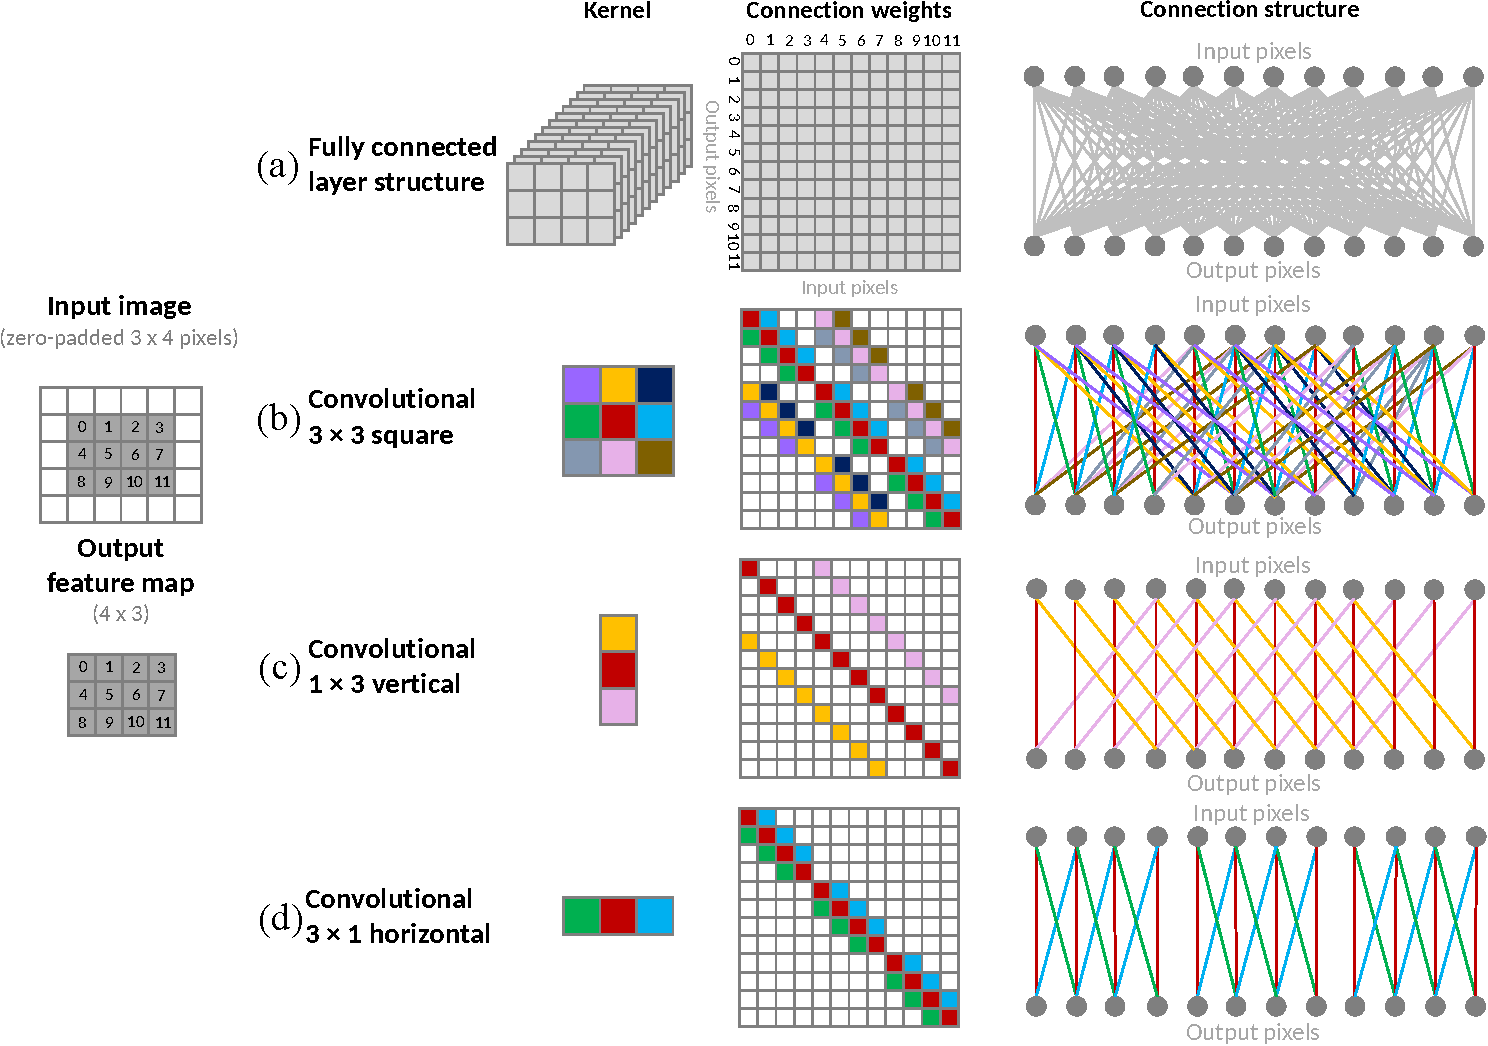
\includegraphics[width=0.61\columnwidth]{sparseconn3}
        }
        \caption[Image access map visualizing sparsity of convolutional filters.]{
            {\bf Network connection structure for convolutional layers.} An input image is transformed in one layer of an neural network into an output image of same size. Connection weight maps show pairwise dependencies between input and output pixels. In (a), each node is connected to all input pixels. For (b,c,d), output pixels depend only on a subset of input pixels (shared weights are represented by unique colours). Note that sparsity increases from (a) to (d), opening up potentially more efficient implementation.
        }
        \label{fig:sparseconn}
    \end{figure}
    %%%
    
    Our contributions include a novel method of learning a set of small basis filters that are combined to represent larger filters efficiently. Rather than approximating previously trained networks, we train networks \emph{from scratch} and show that our convolutional layer representation can improve both efficiency and classification accuracy. We further describe how to initialize connection weights effectively for training networks with composite convolutional layers containing groups of differently-shaped filters, which we found to be of critical importance to our training method.
    
    \subsection{Related Work}
    \label{relatedwork}
    There has been much previous work on increasing the test-time efficiency of CNNs. Some promising approaches work by making use of more hardware-efficient representations. For example \citet{1502.02551v1} and \citet{vanhoucke2011improving} achieve training- and test-time compute savings by further quantization of network weights that were originally represented as 32 bit floating point numbers. However, more relevant to our work are approaches that depend on new network connection structures, efficient approximations of previously trained networks, and learning low rank filters. 
    
    \paragraph{Efficient Network Connection Structures.}
    There has been shown to be significant redundancy in the trained weights of CNNs~\citep{Denil2013predicting}. \citet{lecun1989optimal} suggest a method of pruning unimportant connections within networks. However this requires repeated network re-training and may be infeasible for modern, state-of-the-art CNNs requiring weeks of training time. \citet{Lin2013NiN} show that the geometric increase in the number and dimensions of filters with deeper networks can be managed using low-dimensional embeddings. The same authors show that global average-pooling may be used to decrease model size in networks with fully connected layers. \citet{Simonyan2014verydeep} show that stacked filters with small spatial dimensions (\eg $3\times 3$), can operate on the effective receptive field of larger filters (\eg $5 \times 5$) with less computational complexity.
    
    \paragraph{Low-Rank Filter Approximations.}
    \citet{conf/cvpr/RigamontiSLF13} approximate {\em previously trained} CNNs with low-rank filters for the semantic segmentation of curvilinear structures within volumetric medical imagery. They discuss two approaches: enforcing an $L_1$-based regularization to learn approximately low rank filters, which are later truncated to enforce a strict rank, and approximating a set of pre-learned filters with a tensor-decomposition into many rank-1 filters. Neither approach learns low rank filters directly, and indeed the second approach proved the more successful.
    
    The work of \citet{journals/corr/JaderbergVZ14} also approximates the existing filters of previously trained networks. They find separable 1D filters through an optimization minimizing the reconstruction error of the already learned full rank filters. They achieve a 4.5$\times$ speed-up with a loss of accuracy of 1\% in a text recognition problem. However since the method is demonstrated only on text recognition, it is not clear how well it would scale to larger data sets or more challenging problems. A key insight of the paper is that filters can be represented by low rank approximations not only in the spatial domain but also in the channel domain.
    
    Both of these methods show that, at least for their respective applications, low rank approximations of full-rank filters learned in convolutional networks can increase test time efficiency significantly. However, being approximations of pre-trained networks, they are unlikely to improve test accuracy, and can only increase the computational requirements during training.
    
    \paragraph{Learning Separable Filters.}
    \citet{mamalet2012simplifying} propose training networks with separable filters on the task of digit recognition with the MNIST dataset. They train networks with \emph{sequential} convolutional layers of horizontal and vertical 1D filters, achieving a speed-up factor of 1.6$\times$, but with a relative increase in test error of 13\% (1.45\% \vs 1.28\%).Our approach generalizes this, allowing both horizontal and vertical 1D filters (and other shapes too) at the same layer and avoiding issues with ordering.  We also demonstrate a decrease in error and on more challenging datasets.
    
    
    \section{Using Low-Rank Filters in CNNs}
    
    %%% Figure
    \begin{figure}[t] 
        \centering
        \begin{subfigure}[l]{0.38\columnwidth}
            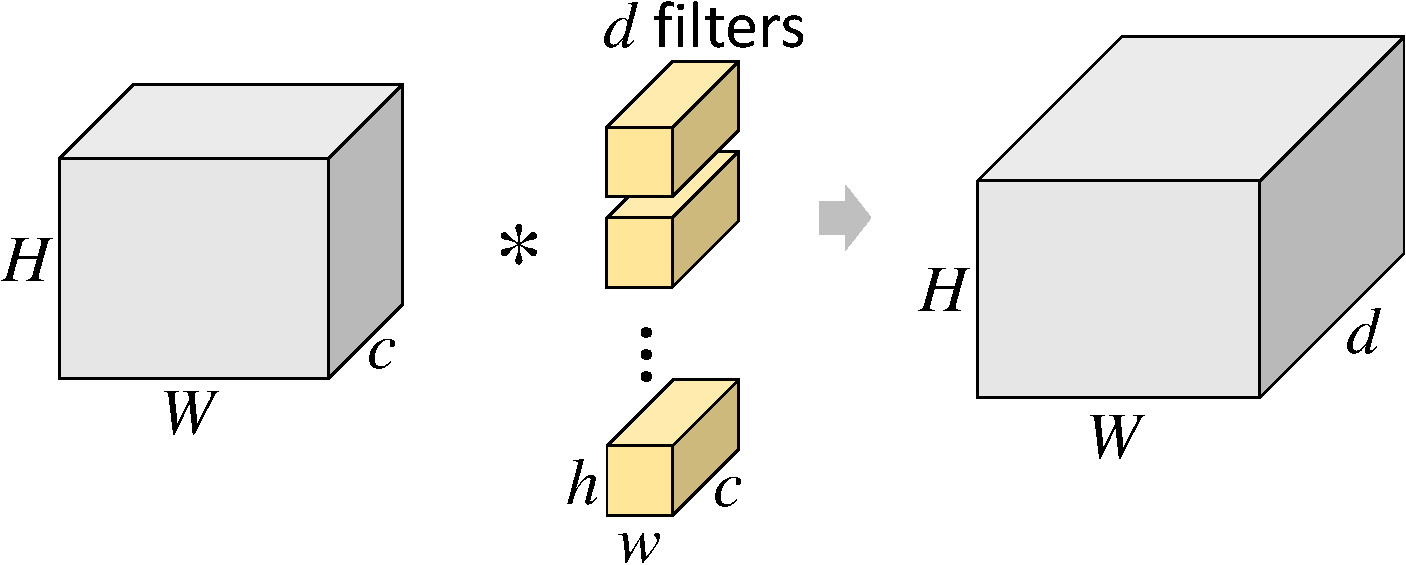
\includegraphics[width=\columnwidth, page=1]{sparsification}
            \caption{A full rank convolutional layer.}
            \label{fig:fullrank}
        \end{subfigure}\\
        \begin{subfigure}[b]{0.6\columnwidth}
            \includegraphics[width=\columnwidth, page=2]{sparsification}
            \caption{Sequential separable filters \citep{journals/corr/JaderbergVZ14}.}
            \label{fig:separableseq}
        \end{subfigure}\\
        \begin{subfigure}[b]{0.6\columnwidth}
            \includegraphics[width=\columnwidth, page=3]{sparsification}
            \caption{Our method, a learned basis space of filters that are rectangular in the spatial domain and oriented horizontally and vertically.}
            \label{fig:ourmethod}
        \end{subfigure}\\
        \begin{subfigure}[b]{0.6\columnwidth}
            \includegraphics[width=\columnwidth, page=4]{sparsification}
            \caption{Our method, a learned basis space of vertical/horizontal rectangular filters and square filters. Filters of other shapes are also possible.}
            \label{fig:ourmethodfullrank}
        \end{subfigure}
        \caption[Overview of methods of using low-rank filters.]{{\bf Methods of using low-rank filters in CNNs}. The activation function is not shown, coming after the last layer in each configuration.} 
        \label{fig:separablemethods}
    \end{figure}
    %%%
    
    \subsection{Convolutional Filters}
    
    The convolutional layers of a CNN produce output `images' (usually called {\em feature maps}) by convolving input images with one or more learned filters. %The output images of convolutional layers are  to distinguish them from raw input images.
    In a typical convolutional layer, as illustrated in Fig.~\ref{fig:fullrank}, a $c$-channel input image of size $H \times W$ pixels is convolved with $d$ filters of size $h \times w \times c$ to create a $d$-channel output image. Each filter is represented by $h w c$ independent weights. Therefore the computational complexity for the convolution of the filter with a $c$-channel input image is $\mathcal{O}(d w h c)$ (per pixel in the output feature map).
    
    In what follows, we describe schemes for modifying the architecture of the convolutional layers so as to reduce computational complexity. The idea is to replace full-rank convolutional layers with modified versions that represent the same number of filters by linear combinations of basis vectors, \ie as lower rank representations of the full rank originals.
    
    \subsection{Sequential Separable Filters}
    \label{seqsep}
    An existing scheme for reducing the computational complexity of convolutional layers \citep{journals/corr/JaderbergVZ14} is to replace each one with a sequence of two regular convolutional layers but with filters that are rectangular in the spatial domain, as shown in Fig \ref{fig:separableseq}. The first convolutional layer has $m$ filters of size $w \times 1 \times c$, producing an output feature map with $m$ channels. The second convolutional layer has $d$ filters of size $1 \times h \times m$, producing an output feature map with $d$ channels. By this means the full rank original convolutional filter bank is represented by a low rank approximation formed from a linear combination of a set of separable $w \times h$ basis filters.  The computational complexity of this scheme is $\mathcal{O}(m c w)$ for the first layer of horizontal filters and $\mathcal{O}(d m h)$ for the second layer of vertical filters, with a total of $\mathcal{O}(m(c w + d h))$.
    
    Note that \citet{journals/corr/JaderbergVZ14} use this scheme to approximate existing full rank filters belonging to previously trained networks using a retrospective fitting step. In this work, by contrast,  we {\em train} networks containing convolutional layers with this architecture from scratch. In effect, we learn the separable basis filters and their combination weights simultaneously during network training.
    
    
    \subsection{Filters as Linear Combinations of Bases}
    In this work we introduce another scheme for reducing convolutional layer complexity. This works by representing convolutional filters as linear combinations of basis filters as illustrated in Fig.~\ref{fig:ourmethod}. This scheme uses \emph{composite layers} comprising several sets of filters where the filters in each set have different spatial dimensions (see Fig.~\ref{fig:compositelayers}). The outputs of these basis filters may be combined in a subsequent layer containing filters with spatial dimensions $1 \times 1$.
    
    This is illustrated in Fig.~\ref{fig:ourmethod}. Here, our composite layer contains horizontal $w\times 1$ and vertical $1\times h$ filters, the outputs of which are concatenated in the channel dimension, resulting in an intermediate $m$-channel feature map. These filter responses are then linearly combined by the next layer of $d$ $1\times 1$ filters to give a $d$-channel output feature map. In this case, the filters are applied on the input feature map with $c$ channels and followed by a set of $m$ 1$\times$1 filters over the $m$ output channels of the basis filters. If the number of horizontal and vertical filters is the same, the computational complexity is $\mathcal{O}( m(wc/2 +hc/2 + d))$.
    Interestingly, the configuration of Fig.~\ref{fig:ourmethod} gives rise to linear combinations of horizontal and vertical filters that are cross-shaped in the spatial domain. This is illustrated in Fig.~\ref{fig:conv1filters} for filters learned in the first convolutional layer of the`vgg-gmp-lr-join' model that is described in the Results section when it is trained using ILSVRC dataset.
    
    \begin{figure}[tb] 
        \centering
        \begin{tabular}[c]{rl}
            &
            \subcaptionbox{$3\times1$ filters.\label{fig:horizontalfilters}}
            {
                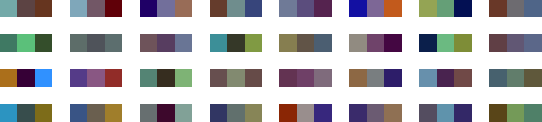
\includegraphics[width=0.3\columnwidth]{conv1_x}
            }\\
            \subcaptionbox{$1\times3$ filters.\label{fig:verticalfilters}}[0.3\columnwidth]
            {
                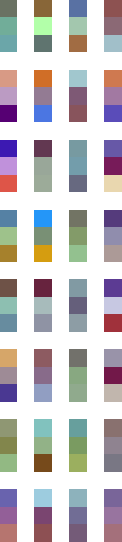
\includegraphics[height=0.3\columnwidth]{conv1_y}
            }&
            \subcaptionbox{Learned linear combinations.\label{fig:linearcomb}}
            {
                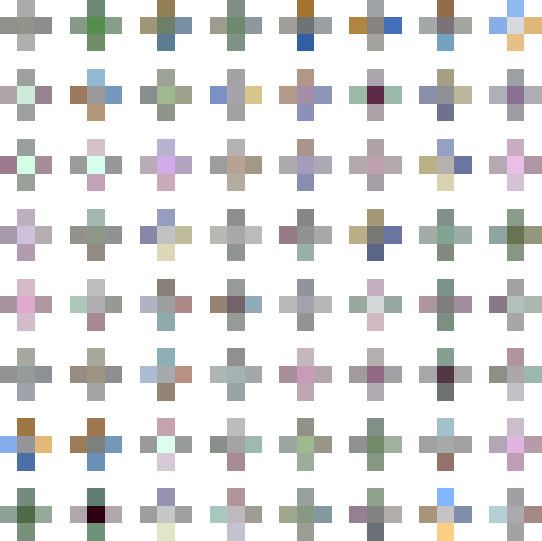
\includegraphics[width=0.3\columnwidth]{linearcombinations}
            }\\
        \end{tabular}
        \caption[Learned Cross-Shaped Filters.]{{\bf Learned Cross-Shaped Filters}. The cross-shaped filters (c) learned as weighted linear combination of (b) $1 \times 3$ and (c) $3 \times 1$ basis filters in the first convolutional layer of the the `vgg-gmp-lr-join' model trained using the ILSVRC dataset.}
        \label{fig:conv1filters}
    \end{figure}
    
    Note that, in general, more than two different sizes of basis filter might be used in the composite layer. For example,  Fig.~\ref{fig:ourmethodfullrank} shows a combination of three sets of filters with spatial dimensions $w \times 1$, $1 \times h$, and $w \times h$. Also note that an interesting option is to omit the $1 \times 1$ linear combination layer and instead allow the connection weights in a subsequent network layer to learn to combine the basis filters of the preceding layer (despite any intermediate non-linearity, \eg ReLUs). This possibility is explored in practice in the Results section.
    
    In that our method uses a combination of filters in a composite layer, it is similar to the `GoogLeNet' of \citet{Szegedy2014going} which uses `inception' modules comprising several (square) filters of different sizes ranging from 1$\times$1 to 5$\times$5. In our case, however, we are implicitly learning linear combinations of less computationally expensive filters with different orientations (\eg 3$\times$1 and 1$\times$3 filters), rather than combinations of filters of different sizes. Amongst networks with similar computational requirements, GoogLeNet is one of the most accurate for large scale image classification tasks (see Fig.~\ref{fig:vggplots}), partly due to the use of heterogeneous filters in the inception modules, but also the use of low-dimensional embeddings and global pooling.

    \section{Training CNNs with mixed-shape low-rank filters}
    \label{initialization}
    To determine the standard deviations to be used for weight initialization, we use an approach similar to that described by \citet{glorot2010understanding} (with the adaptation described by \citet{He2015delving} for layers followed by a ReLU). In Appendix \ref{initializationderivation}, we show the details of our derivation, generalizing the approach of \citet{He2015delving} to the initialization of `composite' layers comprising several groups of filters of different spatial dimensions (see Appendix \ref{initializationderivation}, Fig.~\ref{fig:compositelayers}). This is one of the main contributions of this work.
    \section{Initializing CNNs with mixed-shape low-rank filters}
    \label{initializationderivation}
    At the start of training, network weights are initialized at random using samples drawn from a Gaussian distribution with a standard deviation parameter specified separately for each layer. We found that the setting of these parameters was critical to the success of network training and difficult to get right, particularly because published parameter settings used elsewhere were not suitable for our new network architectures. With unsuitable weight initialization, training may fail due to {\em exploding gradients}, where  back propagated gradients grow so large as to cause numeric overflow, or {\em vanishing gradients} where back propagated gradients grow so small that their effect is dwarfed by that of weight decay such that loss does not decrease during training \citep{Hochreiter01gradientflow}.
    
    To determine the standard deviations to be used for weight initialization, we use an approach similar to that described by \citet{glorot2010understanding} (with the adaptation described by \citet{He2015delving} for layers followed by a ReLU). Their approach works by ensuring that the magnitudes of back-propagated gradients remain approximately the same throughout the network. Otherwise, if the gradients were inappropriately scaled by some factor (\eg $\beta$) then the final back-propagated signal would be scaled by a potentially much larger factor ($\beta^L$ after $L$ layers).
    
    In what follows, we adopt notation similar to that of \citet{He2015delving}, and follow their derivation of the appropriate standard deviation for weight initialization. However, we also generalize their approach to the initialization of `composite' layers comprising several groups of filters of different spatial dimensions (see Fig.~\ref{fig:compositelayers}). This is one of the main contributions of this work.
    
    \paragraph{Forward Propagation.}
    The response of the $l^\text{th}$ convolutional layer can be represented as
    \begin{equation}
    \mathbf{y}_l =\mathbf{W}_l \mathbf{x}_l + \mathbf{b}_l.
    \end{equation}
    Here $\mathbf{y}_l$ is a $d \times 1$ vector representing a pixel in the output feature map and $\bf x_l$ is a $ w h c \times 1$ vector that represents a $w \times h$ subregion of the $c$-channel input feature map. $\mathbf{W}_l$ is the $d\times n$ weight matrix, where $d$ is the number of filters and $n$ is the size of a filter, \ie $n = w h c$ for a filter with spatial dimensions $w \times h$ operating on an input feature map of $c$ channels, and $\mathbf{b}_l$ is the bias. Finally $\mathbf{x}_l = f(\mathbf{y}_{l-1})$ is the output of the previous layer passed through an activation function $f$ (\eg the application of a ReLU to each element of $\mathbf{y}_{l-1}$).
    
    \paragraph{Backward Propagation.}
    During back-propagation, the gradient of a convolutional layer is computed as
    \begin{equation}
    \Delta \mathbf{x}_l = \hat{\mathbf{W}}_l \Delta \mathbf{y}_l,
    \label{eq:back_prop_gradient}
    \end{equation}
    where $\Delta \mathbf{x}_l$ and $\Delta \mathbf{y}_l$ denote the derivatives of loss $\cal L$ with respect to input and output pixels. $\Delta \mathbf{x}_l$ is a $c \times 1$ vector of gradients with respect to the channels of a single pixel in the input feature map and $\Delta \mathbf{y}$ represents $h \times w$ pixels in d channels of the output feature map. $\hat{\mathbf{W}}_l$ is a $c \times \hat{n}$ matrix where the filter weights are arranged in the right order for back-propagation, and $\hat{n} = whd$. Note that $\hat{\mathbf{W}}_l$ can be simply reshaped from $\mathbf{W}_l^\top$. Also note that the elements of $\Delta \mathbf{y}_l$ correspond to pixels in the output image that had a forwards dependency on the input image pixel corresponding to $\Delta \mathbf{x}$. In back propagation, each element $\Delta y_l$ of $\Delta \mathbf{y}_l$ is related to an element $\Delta x_{l+1}$ of some $\Delta \mathbf{x}_{l+1}$ (\ie a back-propagated gradient in the next layer) by the derivative of the activation function $f$:
    \begin{equation}
    \Delta y_l = f^\prime (y_l) \Delta x_{l+1},
    \end{equation}
    where $f^\prime$ is the derivative of the activation function. 
    
    
    \newcommand{\Expect}{\mathrm{E}}
    \newcommand{\Var}{\mathrm{Var}}
    
    \paragraph{Weight Initialization.}
    Now let $\Delta y_l$, $\Delta x_l$ and $w_l$ be scalar random variables that describe the distribution of elements in $\Delta \mathbf{y}_l$, $\Delta \mathbf{x}_{l}$ and $\hat{\mathbf{W}}_l$ respectively. Then, assuming $f^\prime (y_l)$ and $\Delta x_{l+1}$ are independent,
    \begin{equation}
    \Expect[\Delta y_l] = \Expect[f^\prime (y_l)] \Expect[ \Delta x_{l+1}].
    \end{equation}
    
    For the ReLU case, $f'(y_l)$ is zero or one with equal probability. 
    Like \citet{glorot2010understanding}, we assume that $w_l$ and $\Delta y_l$ are independent of each other. Thus, equation \ref{eq:back_prop_gradient} implies that $\Delta x_l$ has zero mean for all $l$, when $w_l$ is initialized by a distribution that is symmetric around zero. Thus we have $\Expect[\Delta y_l] = \frac{1}{2}\Expect[\Delta x_{l+1}]= 0$ and also $\Expect[(\Delta y_l)^2] = \Var[\Delta y_l] = \frac{1}{2} \Var[\Delta x_{l+1}]$. Now, since each element of $\Delta \mathbf{x}_l$ is a summation of $\hat n$ products of elements of $\hat{\mathbf{W}}_l$ and elements of $\Delta \mathbf{y}_l$, we can compute the variance of the gradients in equation \ref{eq:back_prop_gradient}:
    
    \begin{equation}
    \begin{aligned}
    \Var[\Delta x_l] &=  \hat{n} \Var[w_l] \Var[\Delta y_l]\\
    &= \frac{1}{2}   \hat{n} \Var[w_l] \Var [\Delta x_{l+1}].
    \end{aligned}
    \end{equation}
    
    
    To avoid scaling the gradients in the convolutional layers (to avoid exploding or vanishing gradients), we set the ratio between these variances to 1:
    \begin{equation}
    \frac{1}{2} \hat{n} \Var[w_l] = 1.
    \end{equation}
    
    This leads to the result of \citet{He2015delving}, in that a layer with $\hat{n}_l$ connections followed by a ReLU activation function should be initialized with a zero-mean Gaussian distribution with standard deviation $\sqrt{2/ \hat{n}_l}$.
    
    \paragraph{Weight Initialisation in Composite Layers.}
    %%% Figure
    \begin{figure}[tb!]
        \centering
        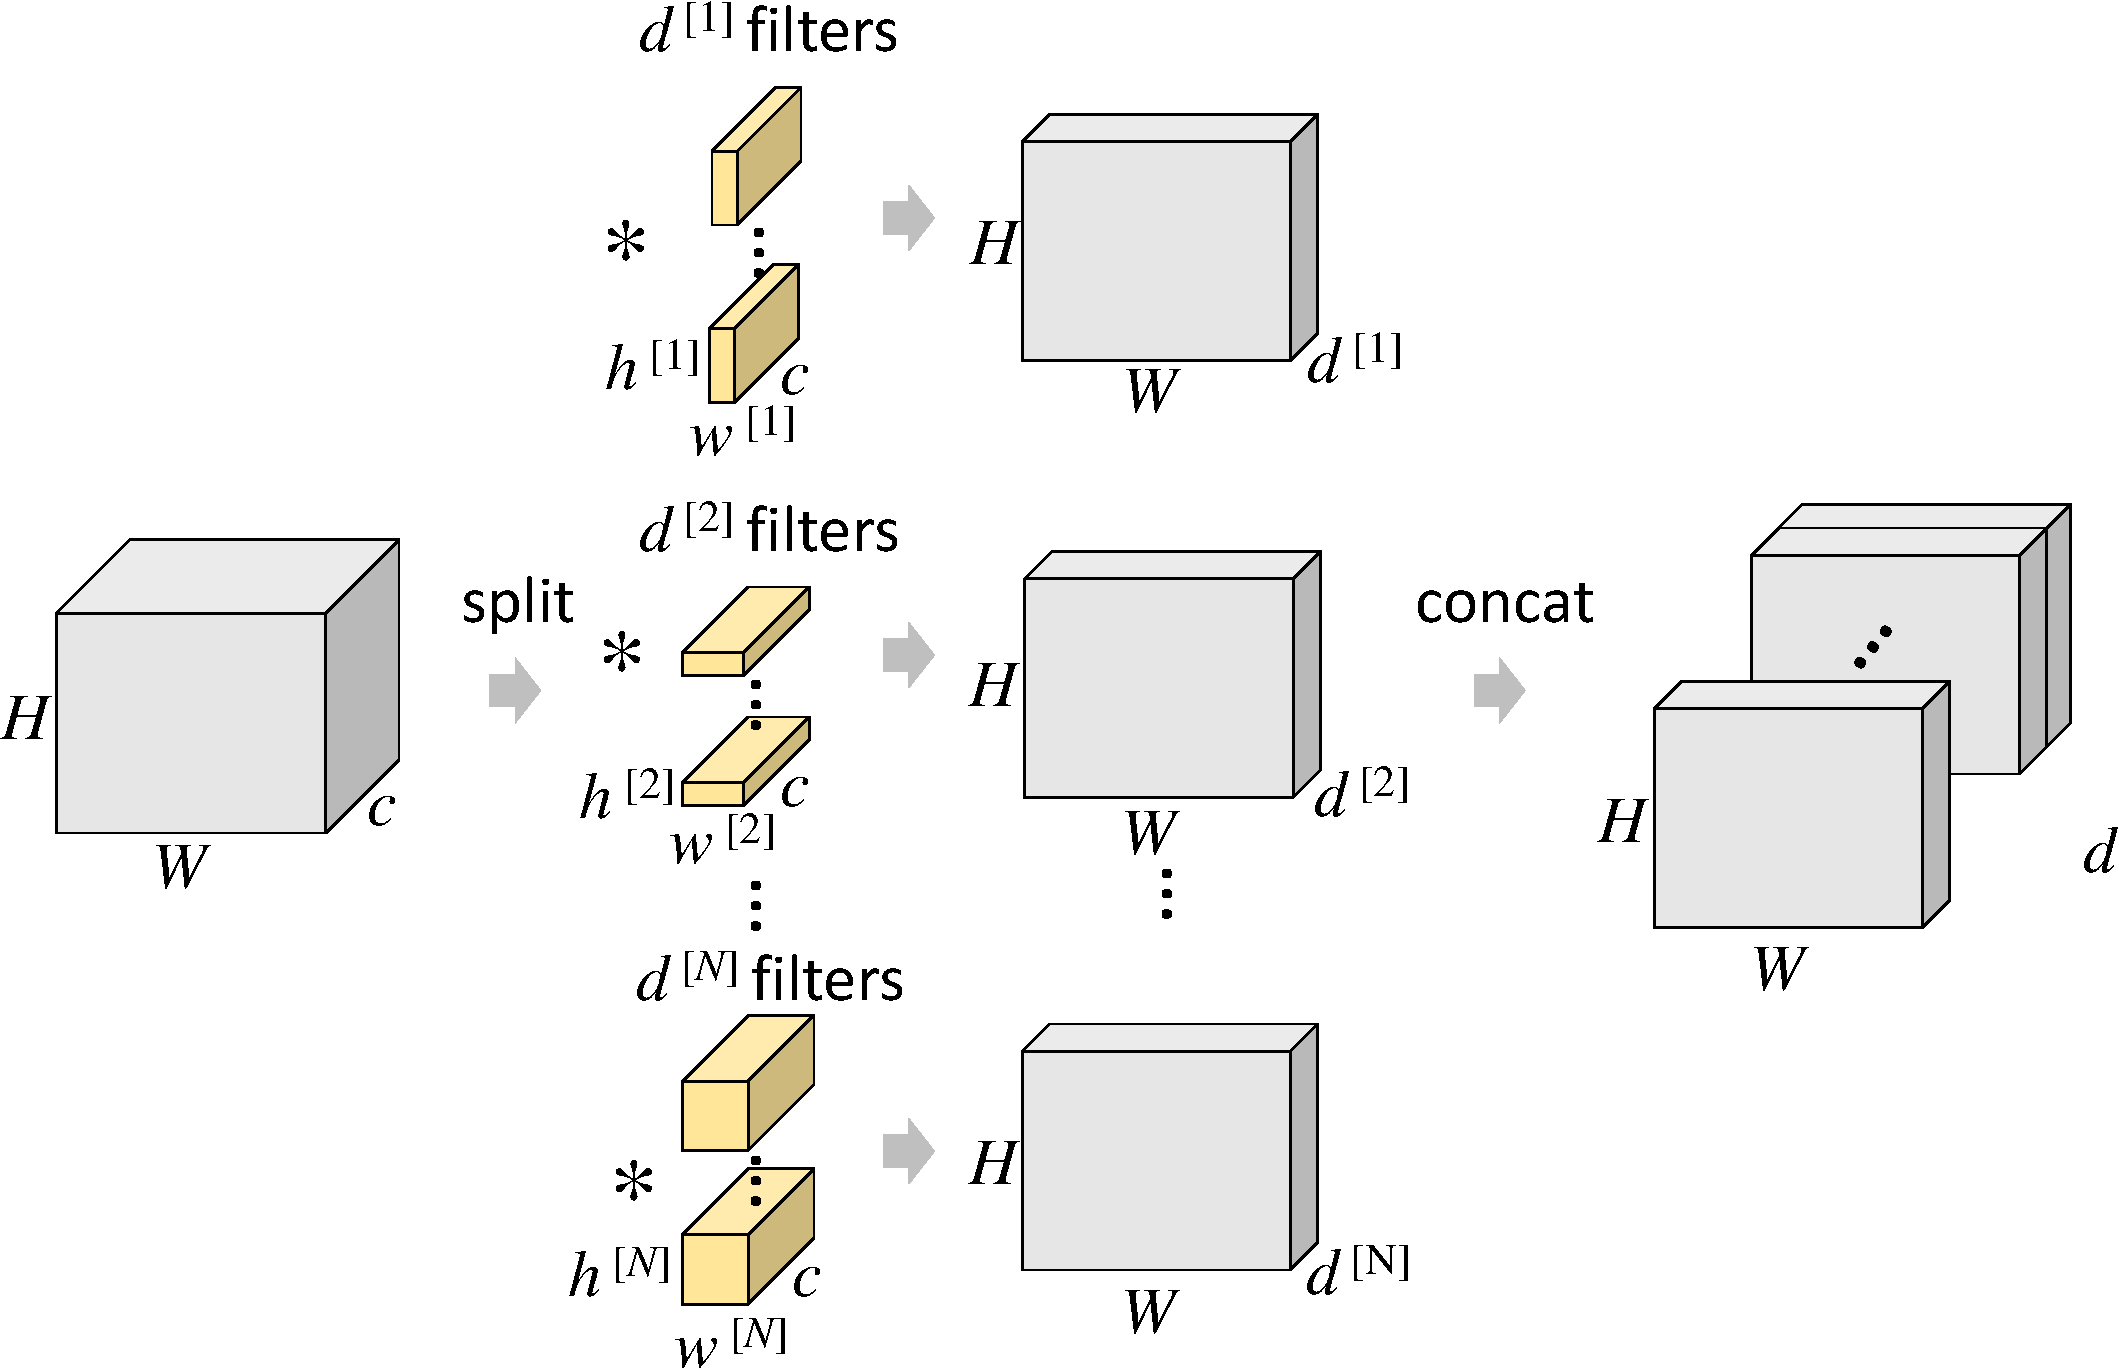
\includegraphics[width=0.7\columnwidth]{composite}
        \caption[Composite Layer.]{{\bf A composite layer}. Composite layers convolve an input feature map with $N$ groups of convolutional filters of several different spatial dimensions. Here the $i^\text{th}$ group has $d^{[i]}$ filters with spatial dimension $w^{[i]} \times h^{[i]}$. The outputs are concatenated to create a $d$ channel output feature map. Composite layers require careful weight initialization to avoid vanishing/exploding gradients during training.}
        \label{fig:compositelayers}
    \end{figure}
    %%%
    
    The initialization scheme described above assumes that the layer comprises filters of spatial dimension $w \times h$. Now we extend this scheme to composite convolutional layers containing $N$ groups of filters of different spatial dimensions $w^{[i]} \times h^{[i]}$ (where superscript $[i]$ denotes the group index and with $i\in \{1,\dots,N\}$). Now the layer response is the concatenation of the responses of each group of filters:
    \begin{equation}
    \mathbf{y}_l =\begin{bmatrix}\mathbf{W}_l^{[1]} \mathbf{x}_l^{[1]} \\ \mathbf{W}_l^{[2]} \mathbf{x}_l^{[2]} \\ \dots \\ \mathbf{W}_l^{[N]} \mathbf{x}_l^{[N]} \end{bmatrix} + \mathbf{b}_l.
    \end{equation}
    As before $\mathbf{y}_l$ is a $d \times 1$ vector representing the response at one pixel of the output feature map. Now each ${\bf x}^{[i]}$ is a $w^{[i]} h^{[i]} c \times 1$ vector that represents a different shaped $w^{[i]} \times h^{[i]}$ sub-region of the input feature map. Each $\mathbf{W}_l^{[i]}$ is the $c_l^{[i]}\times \hat{n}^{[i]}$ weight matrix, where $d$ is the number of filters and $\hat{n}^{[i]}$ is the size of a filter, \ie $\hat{n}^{[i]} = w^{[i]} h^{[i]} c^{[i]}$ for a filter of spatial dimension $w^{[i]} \times h^{[i]}$ operating on an input feature map of $c_l = d_{l-1}$ channels.
    
    During back propagation, the gradient of the composite convolutional layer is computed as a summation of the contributions from each group of filters:
    \begin{equation}
    \Delta \mathbf{x}_l = \hat{\mathbf{W}}_l^{[1]} \Delta \mathbf{y}_l^{[1]} +  \hat{\mathbf{W}}_l^{[2]} \Delta \mathbf{y}_l^{[2]} + \dots+  \hat{\mathbf{W}}_l^{[N]} \Delta \mathbf{y}_l^{[N]},
    \label{eq:back_prop_gradient_composite}
    \end{equation}
    where now $\Delta \mathbf{y}^{[i]}$ represents $w^{[i]} \times h^{[i]}$ pixels in $d^{[i]}$ channels of the output feature map. Each $\hat{\mathbf{W}}_l^{[i]}$ is a $c_l \times \hat{n}^{[i]}$ matrix of weights arranged appropriately for back propagation. Again, note that each $\hat{\mathbf{W}}_l^{[i]}$ can be simply reshaped from $\mathbf{W}_l^{[i]}$.
    
    As before, each element of $\Delta \mathbf{y}_l$ is a sum over $\hat n$ products between elements of $\hat{\mathbf{W}}^{[i]}_l$ and elements of $\Delta \mathbf{y}^{[i]}_l$ and here $\hat{n}$ is given by:
    \begin{equation}
    \hat{n} = \sum{ w^{[i]} h^{[i]} d^{[i]}}.
    \end{equation}
    
    In the case of a ReLU non-linearity, this leads to a zero-mean Gaussian distribution with standard deviation:
    
    \begin{equation}
    \sigma = \sqrt{\frac{2}{\sum{ w^{[i]} h^{[i]} d^{[i]}}}}.
    \end{equation}
    
    In conclusion, a composite layer of heterogeneously-shaped filter groups, where each filter group $i$ has $w^{[i]} h^{[i]} d^{[i]}$ outgoing connections should be initialized as if it is a single layer with  $\hat{n} = \sum{ w^{[i]} h^{[i]} d^{[i]}}$. Thus in the case of a ReLU non-linearity, we find that such a composite layer should be initialized with a zero-mean Gaussian distribution with standard deviation:
    
    \begin{equation}
    \sigma = \sqrt{\frac{2}{\sum{ w^{[i]} h^{[i]} d^{[i]}}}}.
    \end{equation}
    
    \section{Results and Comparisons}
    To validate our approach, we show that we can replace the filters used in existing state-of-the-art network architectures with low-rank representations as described above to reduce computational complexity without reducing accuracy. Here we characterize the computational complexity of a CNN using the number of multiply accumulate operations required for a forward pass (which depends on the size of the filters in each convolutional layer as well as the input image size and stride). However, we have observed strong correlation between multiply-accumulate counts and runtime for both CPU and GPU implementations of the networks described here (as shown in Appendix \ref{mavstimings}, Fig.~\ref{fig:mavstimings}). Note that the Caffe timings differ more for the initial convolutional layers where the input sizes are much smaller (3-channels) as \text{BLAS} is less efficient for the relatively small matrices being multiplied.
    
    \paragraph{Methodology.} We augment our training set with randomly cropped and mirrored images, but do not use any scale or photometric augmentation, or over-sampling. This allows us to compare the efficiency of different network architectures without having to factor in the computational cost of the various augmentation methods used elsewhere. During training, for every model except GoogLeNet, we adjust the learning rate according to the schedule $\gamma_t = \gamma_0(1+\gamma_0\lambda t)^{-1}$, where $\gamma_0,\gamma_t$ and $\lambda$ are the initial learning rate, learning rate at iteration $t$, and weight decay respectively~\citep{Bottou2012sgdtricks}. When the validation accuracy levels off we manually reduce the learning rate by further factors of 10 until the validation accuracy no longer increases. Unless otherwise indicated, aside from changing the standard deviation of the normally distributed weight initialization, as explained in \S\ref{initialization}, we used the standard hyper-parameters for each given model. Our results use no test-time augmentation.  
    
    \subsection{VGG-11 Architectures for ILSVRC Object Classification and MIT Places Scene Classification}
    \label{vggresults}
    We evaluated classification accuracy of the VGG-11 based architectures using two datasets, ImageNet Large Scale Visual Recognition Challenge 2012 (`ILSVRC') and MIT Places. The ILSVRC dataset comprises 1.2M training images of 1000 object classes, commonly evaluated by top-1 and top-5 accuracy on the 50K image validation set. The MIT Places dataset comprises 2.4M training images from 205 scene classes, evaluated with top-1 and top-5 accuracy on the 20K image validation set.
    
    VGG-11 (`VGG-A') is an 11-layer convolutional network introduced by \citet{Simonyan2014verydeep}. It is in the same family of network architectures used by \citet{Simonyan2014verydeep,He2015delving} to obtain the state-of-the-art accuracy for ILSVRC, but uses fewer convolutional layers and therefore fits on a single GPU during training. During training of our VGG-11 based models, we used the standard hyperparameters as detailed by \citet{Simonyan2014verydeep} and the initialization of \citet{He2015delving}.
    
    In what follows, we compare the accuracy of a number of different network architectures detailed in Appendix~\ref{vggmodeltable}, Table~\ref{table:vggarch}. Results for ILSVRC are given in Table~\ref{table:vggimagenetresults}, and plotted in Fig.~\ref{fig:vggplots}. Results for MIT Places are given in Table \ref{table:placesresults}, and plotted in Fig.~\ref{fig:placesresults}. 
    
    \paragraph{Baseline (Global Max Pooling).}  Compared to the version of the network described in \citep{Simonyan2014verydeep}, we use a variant that replaces the final $2 \times 2$ max pooling layer before the first fully connected layer with a global max pooling operation, similar to the global average pooling used by \citet{Lin2014,Szegedy2014going}. We evaluated the accuracy of the baseline VGG-11 network with global max-pooling (\textbf{vgg-gmp}) and without (\textbf{vgg-11}) on the two datasets. We trained these networks at stride 1 on the ILSVRC dataset and at stride 2 on the larger MIT Places dataset. This globally max-pooled variant of VGG-11 uses over 75\% fewer parameters than the original network and gives consistently better accuracy -- almost 3 percentage points lower top-5 error on ILSVRC than the baseline VGG-11 network on ILSVRC (see Table~\ref{table:vggimagenetresults}). We used this network as the baseline for the rest of our experiments.
    
    
    \paragraph{Separable Filters.} To evaluate the separable filter approach described in \S \ref{seqsep} (illustrated in Fig.~\ref{fig:separablemethods}b), we replaced each convolutional layer in VGG-11 with a sequence of two layers, the first containing horizontally oriented $1 \times 3$ filters and the second containing vertically oriented $3 \times 1$ filters (\textbf{vgg-gmp-sf}). These filters applied in sequence represent $3 \times 3$ kernels using a low dimensional basis space. Unlike \citet{journals/corr/JaderbergVZ14}, we trained this network from scratch instead of approximating the full-rank filters in a previously trained network. Compared to the original VGG-11 network, the separable filter version requires approximately 14\% less compute. Results are shown in Table~\ref{table:vggimagenetresults} for ILSVRC and Table~\ref{table:placesresults} for MIT Places. Accuracy for this network is approx.~0.8\% lower than that of the baseline vgg-11-gmp network for ILSVRC and broadly comparable for MIT Places. This approach does not give such a significant reduction in computational complexity as what follows, but it is nonetheless interesting that separable  filters are capable of achieving quite high classification accuracy on such challenging tasks.
    
    \paragraph{Simple Horizontal/Vertical Basis.} To demonstrate the efficacy of the simple low rank filter representation illustrated in Fig.~\ref{fig:separablemethods}c, we created a new network architecture (\textbf{vgg-gmp-lr-join}) by replacing each of the convolutional layers in VGG-11 (original filter dimensions were $3 \times 3$) with a sequence of two layers. The first layer comprises half $1\times 3$ filters and half $3\times 1$ filters whilst the second layer comprises the same number of $1\times 1$ filters. The resulting network is approximately 49\% faster than the original and yet it gives broadly comparable accuracy (within 1 percentage point) for both the ILSVRC and MIT Places datasets.
    
    \paragraph{Full-Rank Mixture.} An interesting question concerns the impact on accuracy of combining a small proportion of 3×3 filters with the 1×3 and 3×1 filters used in ‘vgg-gmp-lr-join’. To answer this question, we trained a network, \textbf{vgg-gmp-lr-join-wfull}, with a mixture of 25\% $3 \times 3$ and 75\% $1 \times 3$ and $3 \times 1$ filters, while preserving the total number of filters of the baseline network (as illustrated in Fig.~\ref{fig:ourmethodfullrank}). This network was significantly more accurate than both `vgg-gmp-lr-join' and the baseline, with a top-5 center crop accuracy of 89.7\% on ILSVRC, with a computational savings of approx.~16\% over our baseline. We note that the accuracy is approx.~1 percentage point higher than GoogLeNet.
    
    \paragraph{Implicitly Learned Combinations.} In addition, we try a network similar to vgg-gmp-lr-join but without the $1 \times 1$ convolutional layer (as shown in Fig.~\ref{fig:ourmethod}) used to sum the contributions of $3 \times 1$ and $1 \times 3$ filters (\textbf{vgg-gmp-lr}). Interestingly, because of the elimination of the extra $1\times 1$ layers, this gives an additional compute saving such that this model is is only $1/3^{\textrm{rd}}$ of the compute of our baseline, with no reduction in accuracy. This seems to be a consequence of the fact that the subsequent convolutional layer is itself capable of learning effective combinations of filter responses even after the intermediate ReLU non-linearity.
    
    We also trained such a network with double the number of convolutional filters (\textbf{vgg-gmp-lr-2x}), \ie with an equal number of $1 \times 3$ and $3 \times 1$ filters, or $2c$ filters as shown in Fig.~\ref{fig:ourmethod}. We found this to increase accuracy further (88.9\% Top-5 on ILSVRC) while still being approximately 58\% faster than our baseline network.
    
    \paragraph{Low-Dimensional Embeddings.}
    We attempted to reduce the computational complexity of our `gmp-lr' network further in the \textbf{vgg-gmp-lr-lde} network by using a stride of 2 in the first convolutional layer, and adding low-dimensional embeddings, as in \citet{Lin2014,Szegedy2014going}. We reduced the number of output channels by half after each convolutional layer using $1 \times 1$ convolutional layers, as detailed in Appendix~\ref{vggmodeltable}, Table~\ref{table:vggarch}. While this reduces computation significantly, by approx.~86\% compared to our baseline, we saw a decrease in top-5 accuracy on ILSVRC of 1.2 percentage points. We do note however, that this network remains 2.5 percentage points more accurate than the original VGG-11 network, but is 87\% faster.
    
    \begin{table}[htb]
        \centering
        %\resizebox{\columnwidth}{!}{
        \pgfplotstableread[col sep=comma]{lrdata/vggma.csv}\data
        \pgfplotstabletypeset[
        every head row/.style={
            before row=\toprule,after row=\midrule},
        every last row/.style={
            after row=\bottomrule},
        every first row/.style={
            after row=\bottomrule},
        %dec sep align,      % Align at decimal point
        fixed zerofill,     % Fill numbers with zeros
        columns={Network, Stride, Multiply-Acc., Param., Top-1 Acc., Top-5 Acc.},
        column type/.add={lrrrrrr}{},
        columns/Multiply-Acc./.style={
            column name=Multiple-Acc. {\small $\times 10^{9}$},
            preproc/expr={{##1/1e9}}
        },
        columns/Param./.style={
            column name=Param. {\small $\times 10^{7}$},
            preproc/expr={{##1/1e7}}
        },
        columns/Network/.style={string type},
        columns/Stride/.style={precision=0},
        columns/Top-1 Acc./.style={precision=3},
        columns/Top-5 Acc./.style={precision=3},
        highlight col max ={\data}{Top-1 Acc.},
        highlight col max ={\data}{Top-5 Acc.},
        highlight col min ={\data}{Param.},
        highlight col min ={\data}{Multiply-Acc.},
        col sep=comma]{\data}
        %}
        \caption[VGG ILSVRC Results]{{\bf VGG ILSVRC Results.} Accuracy, multiply-accumulate count, and number of parameters for the baseline VGG-11 network (both with and without global max pooling) and more efficient versions created by the methods described in this paper.}
        \label{table:vggimagenetresults}
    \end{table}
    
    \begin{figure}[htb!] 
        \centering
        \pgfplotstableread[col sep=comma]{lrdata/vggma.csv}\datatable
        \pgfplotsset{major grid style={dotted,red}}
        
        \begin{tikzpicture}
        \begin{axis}[
        width=\columnwidth,
        height=0.33\columnwidth,
        axis x line=bottom,
        ylabel=Top-5 Error,
        xlabel=Multiply-Accumulate Operations,
        axis lines=left,
        enlarge x limits=0.10,
        grid=major,
        %xmin=0,
        ytick={0.01,0.02,...,0.21},
        ymin=0.1,ymax=0.15,
        yticklabel={\pgfmathparse{\tick*100}\pgfmathprintnumber{\pgfmathresult}\%},style={
            /pgf/number format/fixed,
            /pgf/number format/precision=1
        },
        legend style={at={(0.01,0.98)}, anchor=north west, column sep=0.5em},
        legend columns=2,
        ]
        \addplot[mark=square*,mark options={fill=blue},nodes near coords,only marks,
        point meta=explicit symbolic,
        x filter/.code={
            \ifnum\coordindex>2\def\pgfmathresult{}\fi
        },
        ] table[meta=Network,x=Multiply-Acc.,y expr={1 - \thisrow{Top-5 Acc.} },]{\datatable};
        \addplot[mark=*,mark options={fill=green},nodes near coords,only marks,
        point meta=explicit symbolic,
        x filter/.code={
            \ifnum\coordindex<3\def\pgfmathresult{}\fi
        },
        ] table[meta=Network,x=Multiply-Acc.,y expr={1 - \thisrow{Top-5 Acc.} },]{\datatable};
        \legend{Baseline Networks, Our Results}
        \end{axis}
        \end{tikzpicture}
        \caption{\textbf{VGG ILSVRC Results.} Multiply-accumulate operations \vs top-5 error for VGG-derived models on ILSVRC object classification dataset, the most efficient networks are closer to the origin. Our models are significantly faster than the baseline network, in the case of `gmp-lr-2x' by a factor of almost 60\%, while slightly lowering error. Note that the `gmp-lr' and `gmp-lr-join' networks have the same accuracy, showing that an explicit linear combination layer may be unnecessary.}
        \label{fig:vggplots}
    \end{figure}
    
    \begin{table}[htbp]
        \centering
        %\resizebox{\columnwidth}{!}{
        \pgfplotstableread[col sep=comma]{lrdata/mitma.csv}\data
        \pgfplotstabletypeset[
        every head row/.style={
            before row=\toprule,after row=\midrule},
        every last row/.style={
            after row=\bottomrule},
        fixed zerofill,     % Fill numbers with zeros
        columns={Network, Stride, Multiply-Acc., Param., Top-1 Acc., Top-5 Acc.},
        column type/.add={lrrrrrr}{},
        columns/Multiply-Acc./.style={
            column name=Multiple-Acc. {\small $\times 10^{8}$},
            preproc/expr={{##1/1e8}}
        },
        columns/Param./.style={
            column name=Param. {\small $\times 10^{7}$},
            preproc/expr={{##1/1e7}}
        },
        columns/Network/.style={string type},
        columns/Stride/.style={precision=0},
        columns/Top-1 Acc./.style={precision=3},
        columns/Top-5 Acc./.style={precision=3},
        highlight col max ={\data}{Top-1 Acc.},
        highlight col max ={\data}{Top-5 Acc.}, 
        highlight col min ={\data}{Param.}, 
        highlight col min ={\data}{Multiply-Acc.}, 
        col sep=comma]{\data}
        %}
        \caption[MIT Places results]{{\bf MIT Places Results.} Accuracy, multiply-accumulate operations, and number of parameters for the baseline `vgg-11-gmp' network, separable filter network as described by \citet{journals/corr/JaderbergVZ14}, and more efficient models created by the methods described in this paper. All networks were trained at stride 2 for the MIT Places dataset.
        }
        \label{table:placesresults}
    \end{table}
    
    
    \subsection{GoogLeNet for ILSVRC Object Classification}
    GoogLeNet, introduced by \citet{Szegedy2014going}, is the most efficient network for ILSVRC, getting close to state-of-the-art results with a fraction of the compute and model size of even VGG-11. The GoogLeNet inception module is a composite layer of 5 homogeneously-shaped filters, $1\times 1$, $3\times 3$, $5\times 5$, and the output of a 3x3 average pooling operations. All of these are concatenated and used as input for successive layers. 
    
    For the \textbf{googlenet-lr} network, within only the inception modules we replaced each the $3\times 3$ filters with low-rank $3 \times 1$ and $1\times 3$ filters, and replaced the layer of $5\times 5$ filters with a set of low-rank $5 \times 1$ and $1\times 5$ filters. For the \textbf{googlenet-lr-conv1} network, we similarly replaced the first and second layer convolutional layers with $7 \times 1$~/~$1\times 7$ and $3 \times 1$~/~$1\times 3$ layers respectively.
    
    Results are shown in Table~\ref{table:googlenetimagenetresults}. Due to the intermediate losses used for training, which contain the only fully-connected layers in GoogLeNet, test time model size is significantly smaller than training time model size. Table~\ref{table:googlenetimagenetresults} also reports test time model size. The low-rank network delivers comparable classification accuracy using 26\% less compute.  No other networks produce comparable accuracy within an order of magnitude of compute. We note that although the Caffe pre-trained GoogLeNet model~\citep{jia2014caffe} has a top-5 accuracy of 0.889, our training of the same network using the given model definition, including the hyper-parameters and training schedule, but a different random initialization had a top-5 accuracy of 0.883.
    
    \begin{table}[htb]
        \centering
        %\resizebox{\columnwidth}{!}{
        \pgfplotstableread[col sep=comma]{lrdata/googlenetma.csv}\data
        \pgfplotstabletypeset[
        every head row/.style={
            before row=\toprule,after row=\midrule},
        every last row/.style={
            after row=\bottomrule},
        every first row/.style={
            after row=\bottomrule}, 
        fixed zerofill,     % Fill numbers with zeros
        columns={Network, Multiply-Acc., Test Param., Top-1 Acc., Top-5 Acc.},
        columns/Multiply-Acc./.style={
            column name=Multiple-Acc. {\small $\times 10^{9}$},
            preproc/expr={{##1/1e9}}
        },
        columns/Test Param./.style={
            column name=Test Param. {\small $\times 10^{6}$},
            preproc/expr={{##1/1e6}}
        },
        column type/.add={lrrrrrr}{},
        columns/Network/.style={string type},
        columns/Top-1 Acc./.style={precision=3},
        columns/Top-5 Acc./.style={precision=3},
        highlight col max ={\data}{Top-1 Acc.},
        highlight col max ={\data}{Top-5 Acc.}, 
        highlight col min ={\data}{Test Param.}, 
        highlight col min ={\data}{Multiply-Acc.}, 
        col sep=comma]{\data}
        %}
        \caption[GoogLeNet ILSVRC Results]{{\bf GoogLeNet ILSVRC Results.} Accuracy, multiply-accumulate count, and number of parameters for the baseline GoogLeNet network and more efficient versions created by the methods described in this paper.
        }
        \label{table:googlenetimagenetresults}
    \end{table}
    
    \begin{figure}[htbp] 
        \centering
        \pgfplotstableread[col sep=comma]{lrdata/googlenetma.csv}\datatable
        \pgfplotsset{major grid style={dotted,red}}
        
        \begin{tikzpicture}
        \begin{axis}[
        width=\columnwidth,
        height=0.33\columnwidth,
        axis x line=bottom,
        ylabel=Top-5 Error,
        xlabel=Multiply-Accumulate Operations,
        axis lines=left,
        enlarge x limits=0.10,
        grid=major,
        ytick={0.01,0.02,...,0.21},
        ymin=0.10,ymax=0.15,
        yticklabel={\pgfmathparse{\tick*100}\pgfmathprintnumber{\pgfmathresult}\%},style={
            /pgf/number format/fixed,
            /pgf/number format/precision=1
        },
        legend style={at={(0.98,0.98)}, anchor=north east, column sep=0.5em},
        legend columns=2,
        ]
        \addplot[mark=square*,mark options={fill=blue},nodes near coords,only marks,
        point meta=explicit symbolic,
        x filter/.code={
            \ifnum\coordindex>0\def\pgfmathresult{}\fi
        }
        ] table[meta=Network,x=Multiply-Acc.,y expr={1 - \thisrow{Top-5 Acc.} },]{\datatable};
        \addplot[mark=*,mark options={fill=green},nodes near coords,only marks,
        point meta=explicit symbolic,
        x filter/.code={
            \ifnum\coordindex<1\def\pgfmathresult{}\fi
        }
        ] table[meta=Network,x=Multiply-Acc.,y expr={1 - \thisrow{Top-5 Acc.} },]{\datatable};
        \legend{Baseline, Our Results}
        \end{axis}
        \end{tikzpicture}
        
        \caption{\textbf{GoogLeNet ILSVRC Results.} Multiply-accumulate operations \vs top-5 error for GoogLeNet-derived models on ILSVRC object classification dataset.}
        \label{fig:googlenetimagenetresults}
    \end{figure}
    
    \subsection{Network-in-Network for CIFAR-10 Object Classification}
    The CIFAR-10 dataset consists of 60,000 $32\times 32$ images in 10 classes, with 6000 images per class. This is split into standard sets of 50,000 training images, and 10,000 test images~\citep{CIFAR10}. As a baseline for the CIFAR-10 dataset, we used the Network in Network architecture~\citep{Lin2014}, which has a published test-set error of 8.81\%. We also used random crops during training, with which the network has an error of 8.1\%. Like most state of the art CIFAR results, this was with ZCA pre-processed training and test data~\citep{goodfellow2013maxout}, training time mirror augmentation and random sub-crops. The results of our CIFAR experiments are listed in Table~\ref{table:cifarresults} and plotted in Fig.~\ref{fig:cifarresults}.
    
    \begin{table}[htb]
        \centering
        %\resizebox{\columnwidth}{!}{
        \pgfplotstableread[col sep=comma]{lrdata/cifarma.csv}\data
        \pgfplotstabletypeset[
        every head row/.style={
            before row=\toprule,after row=\midrule},
        every last row/.style={
            after row=\bottomrule},    
        every first row/.style={
            after row=\bottomrule},
        fixed zerofill,     % Fill numbers with zeros
        columns={Network, Multiply-Acc., Param., Accuracy},
        columns/Multiply-Acc./.style={
            column name=Multiple-Acc. {\small $\times 10^{8}$},
            preproc/expr={{##1/1e8}}
        },
        columns/Param./.style={
            column name=Param. {\small $\times 10^{5}$},
            preproc/expr={{##1/1e5}}
        },
        column type/.add={lrrr}{},
        columns/Network/.style={string type},
        columns/Accuracy/.style={precision=4}, 
        highlight col max ={\data}{Accuracy}, 
        highlight col min ={\data}{Param.}, 
        highlight col min ={\data}{Multiply-Acc.}, 
        col sep=comma]{\data}
        %}
        \caption[CIFAR-10 Results.]{{\bf Network-in-Network CIFAR-10 Results.} Accuracy, multiply-accumulate operations, and number of parameters for the baseline Network-in-Network model and more efficient versions created by the methods described in this paper.}
        \label{table:cifarresults}
    \end{table}
    
    \begin{figure}[htbp] 
        \centering
        \pgfplotstableread[col sep=comma]{lrdata/cifarma.csv}\datatable
        \pgfplotsset{major grid style={dotted,red}}
        
        \begin{tikzpicture}
        \begin{axis}[
        width=\columnwidth,
        height=0.33\columnwidth,
        axis x line=bottom,
        ylabel=Error,
        xlabel=Multiply-Accumulate Operations,
        axis lines=left,
        enlarge x limits=0.10,
        grid=major,
        ytick={0.01,0.02,...,0.21},
        yticklabel={\pgfmathparse{\tick*100}\pgfmathprintnumber{\pgfmathresult}\%},style={
            /pgf/number format/fixed,
            /pgf/number format/precision=1
        },
        ymin=0.07,ymax=0.1,
        legend style={at={(0.98,0.98)}, anchor=north east, column sep=0.5em},
        legend columns=2,
        ]
        \addplot[mark=square*,mark options={fill=blue},nodes near coords,only marks,
        point meta=explicit symbolic,
        x filter/.code={
            \ifnum\coordindex>1\def\pgfmathresult{}\fi
        }
        ] table[meta=Network,x=Multiply-Acc.,y expr={1 - \thisrow{Accuracy} }]{\datatable};
        \addplot[mark=*,mark options={fill=green},nodes near coords,only marks,
        point meta=explicit symbolic,
        x filter/.code={
            \ifnum\coordindex<2\def\pgfmathresult{}\fi
        }
        ] table[meta=Network,x=Multiply-Acc.,y expr={1 - \thisrow{Accuracy} }]{\datatable};
        \legend{Baseline Networks, Our Results}
        \end{axis}
        \end{tikzpicture}
        \caption[Network-in-Network CIFAR-10 Results]{\textbf{Network-in-Network CIFAR-10 Results.} Multiply-accumulate operations \vs error for Network-in-Network derived models on CIFAR-10 object classification dataset.}
        \label{fig:cifarresults}
    \end{figure}
    
    
    This architecture uses $5\times5$ filters in some layers. We found that we could replace all of these with $3\times 3$ filters, with comparable accuracy. As suggested by \citet{Simonyan2014verydeep}, stacked  $3\times 3$ filters have the effective receptive field of larger filters with less computational complexity. In this \textbf{nin-c3} network, we replaced the first convolutional layer with one $3\times 3$ layer, and the second convolutional layer with two $3\times 3$ layers. This network is 26\% faster than the standard NiN model, with only 54\% of the model parameters. Using our low-rank filters in this network, we trained the \textbf{nin-c3-lr} network, which is of similar accuracy (91.8\% \vs 91.9\%) but is approximately 54\% of the original network's computational complexity, with only 45\% of the model parameters.
    \section{Discussion}
    %We found our network architecture, which learns a small set of $3 \times 3$ basis filters along with many $1\times 3$~/~$3\times 1$ basis filters, gave the most impressive results. Such a model, `vgg-lr-wfull', increased the top-5 center crop validation accuracy on ILSVRC by 1 percentage points in accuracy (89.7\% \vs 88.7\%) while reducing computation by 16\%, over our baseline network with global max-pooling. Although we did not try such a configuration of GoogLeNet, our `googlenet-lr' network using only $1\times 3$~/~$3\times 1$ and $1\times 5$~/~$5\times 1$ basis filters within the inception modules obtained the smallest model size while maintaining comparable accuracy, using 26\% less compute than GoogLeNet and 41\% less model parameters.`
    
    It is somewhat surprising that networks based on learning filters with less representational ability are able to do as well, or better, than CNNs with full $k\times k$ filters on the task of image classification. However, a lot of interesting small-scale image structure is well-characterized by low-rank filters, \eg edges and gradients. Our experiments training a separable (rank-1) model (`vgg-gmp-sf') on ILSVRC and MIT Places show surprisingly high accuracy on what are considered challenging problems -- approx.\ 88\% top-5 accuracy on ILSVRC -- but not enough to obtain comparable accuracies to the models on which they are based.
    
    Given that most discriminative filters learned for image classification appear to be low-rank, we instead structure our architectures with a set of basis filters in the way illustrated in Fig.~\ref{fig:ourmethodfullrank}. This allows our networks to learn the most effective combinations of complex (\eg $k\times k$) and simple (\eg $1\times k$, $k\times 1$) filters. Furthermore, in restricting how many complex spatial filters may be learned, this architecture prevents over-fitting, and helps improve generalization. Even in our models where we do not use square $k\times k$ filters, we obtain comparable accuracies to the baseline model, since the rank-2 cross-shaped filters effectively learned as a combination of $3 \times 1$ and $1 \times 3$ filters are capable of representing more complex local pixel relations than rank-1 filters.
    
    %\section{Conclusion}
    %This paper has presented a method to train convolutional neural networks from scratch using low-rank filters. This is made possible by a new way of initializing the network’s weights which takes into consideration the presence of differently shape filters in composite layers. 
    %Validation on image classification in three popular datasets confirms similar or higher accuracy than state of the art, with much greater computational efficiency. 
    
    %Recent advances in state-of-the-art accuracy with CNNs for image classification have come at the cost of increasingly large and computational complex models. We believe our results to show that learning computationally efficient models with fewer, more relevant parameters, can prevent over-fitting, increase generalization and thus also increase accuracy.
    
    %\subsection*{Future Work}
    %This paper has addressed the spatial extents of convolutional filters in CNNs, however the channel extents also exhibit some redundancy, as highlighted by \citet{journals/corr/JaderbergVZ14}, and exploited in the form of low-dimensional embeddings by \citet{Lin2014,Szegedy2014going}. We intend to further explore how our methods can be extended to learn and combine even smaller basis filters and filters with more diverse shapes.
    
\end{document}

%\documentclass[thesis]{subfiles}

\begin{document}
	
	\chapter{Learning Filters with Limited Channel Extents}
	\label{deeproots}
	
	
	It is well understood that the structure of a neural network is critical to its ability to learn from labelled training data and to generalize. Whilst it has been shown that an infinitely wide hidden layer is a universal approximator~\citep{hornik89a}, in practice wide shallow networks do not learn as well as thinner deeper ones -- as shown by recent research~\citep{Krizhevsky2012imanet,Szegedy2014going,Simonyan2014verydeep,He2015}.
	This does not appear to be a limitation of finite capacity, since deep networks have been shown to be representable by shallow networks~\citep{Ba2013dothey}. Rather it seems to be a consequence of limitations in our methods of learning the weights of deep networks.
	
	It has been shown that a large proportion of the learned weights in deep networks are redundant~\citep{Denil2013predicting} (a property that many have attempted to exploit to make neural networks smaller and more computationally efficient~\cite{Szegedy2014going,Denton2014efficient}). It is unsurprising then that regularization is a critical part of training such networks using large training datasets~\cite{Krizhevsky2012imanet}. Without regularization (e.g. weight decay, dropout~\cite{Hinton2012}) deep networks are susceptible to severe over-fitting (see \S\ref{regularization}). Aside from different training methods, a carefully designed network connection structure can have a regularizing effect in and of itself. Convolutional Neural Networks (CNNs)~\citep{Fuk80,Lecun1998} embody this idea, exploiting prior knowledge of the locality of natural image structure to design neural architectures with more limited, but salient, connectivity than a fully-connected neural network, that is in turn easier to learn. More recently, learning CNNs with low rank filters was found to have a regularizing effect, improving generalization compared to a CNN with only full rank filters~\citep{Ioannou2016}.
	
	With few exceptions, state-of-the-art CNNs for image recognition are largely monolithic -- convolutional neural networks with each filter operating on the feature maps of all filters on a previous layer, presenting no significant per-layer heterogeneity. Interestingly, this is in stark contrast to what we understand of biological neural networks, where we see ``highly evolved arrangements of smaller, specialized networks which are interconnected in very specific ways''~\citep{minsky1988perceptrons}.
	% Try to find a creative commons version of this
	%\begin{figure}[t]
	%\centering
	%\includegraphics[width=0.25\columnwidth, page=1]{figs/tree_root.jpg}
	%\caption{This work introduces the idea of using hierarchical filter grouping to create CNN connection structures that resemble tree roots. Applying the technique to existing state-of-the-art networks allows improved efficiency without compromising accuracy.}
	%\label{fig:tree}
	%\end{figure}
	
	% Maybe we need something like this here too, don't know
	%It has been shown that reducing the co-adaption of filters is beneficial to generalization in deep networks~\citep{Hinton2012,goodfellow2013maxout,Cogswell2016}. Co-adaption occurs when hidden layer filters (or neurons) rely on one another to fit training data, such that their outputs become highly correlated. However, instead of using a modified loss, regularization penalty, or randomized network connectivity during training to prevent co-adaption of features, we take a much more direct approach. We use hierarchical filter groups (see \S\ref{regularizingstructure}) to allow the network itself to learn independent filters. By restricting the connectivity between filters on subsequent layers the network is forced to learn filters of limited dependence. We allow the standard network optimization (\eg SGD) to learn appropriate weights within this restricted architecture.
	
	In this paper we show that simple alterations to the architecture of state-of-the-art CNNs for image recognition can drastically reduce computational cost and model size while maintaining (or even increasing) accuracy, through structure-induced regularization, by reducing the connectivity in monolithic networks to reflect more closely the sparse, localized filter co-dependencies within.
	
	\section{Related Work}
	\label{previouswork}
	
	
	\subsubsection{Reducing Co-dependence in Deep Networks.}
	\label{regularization}
	\citet{Hinton2012} introduced {\em dropout} for regularization of deep networks. When training a network layer with dropout, a random subset of neurons is excluded from both the forward and backward pass for each mini-batch. Effectively a different (random) network topology is trained at each iteration. As the authors observe, this approach has some similarities with that of using model ensembles, another effective way to increase generalization. However, one limitation of dropout is that it increases the number of training iterations required for convergence, typically by a factor of two. Recently, \citet{Szegedy2014going} have suggested that dropout provides little incremental accuracy improvement compared to simply training using {\em batch normalization}. 
	
	\citet{Cogswell2016} observe a correlation between the cross-covariance of hidden unit activations and overfitting. To explicitly reduce the cross-covariance of hidden activations, they train networks with a loss function, based on the covariance matrix of the activations in a hidden layer. \citet{Cogswell2016} use this loss on the fully connected layers at the end of deep networks such as AlexNet and demonstrate an increase in generalization accuracy comparable with that obtained by using dropout.
	
	%:
	%\begin{equation}
	%	C_{i,j} = \frac{1}{N} \sum^N_{n = 0} (h_i^n - \mu_i)(h_j^n - \mu_j),
	%	\label{eqn:covariance}
	%\end{equation}
	%where $n$ is a sample in a mini-batch of size $N$, $i$ and $j$ index a pair of activations within the mini-batch, and $\mu_i$ is the sample mean over the batch. The `DeCov' loss is defined as:
	
	%\begin{equation}
	%	L_{\textrm{\texttt{DeCov}}} = \frac{1}{2} \left( \|C\|^2_F - \|diag(C)\|^2_2 \right).
	%	\label{eqn:decov}
	%\end{equation}
	
	\subsubsection{Reducing Model Size and Computation.}
	\label{regularizingstructure}
	Most previous work on reducing computation in CNNs has focused on the spatial extents of the convolutional filters in the form of low-rank spatial filters~\citep{mamalet2012simplifying,journals/corr/JaderbergVZ14, journals/pami/SironiTRLF15, journals/corr/LebedevGROL14, Ioannou2016}, or exploiting the frequency domain~\cite{mathieu2013fast,rippel2015spectral}. More general methods for speeding up CNNs have used reduced precision numerics~\cite{1502.02551v1} or pre-trained model compression~\cite{Chen2015,Kim2016}. Here we explore methods that reduce the computational impact of the large number of filter channels within state-of-the art networks. In particular, methods to decrease the number of filters and thus output feature map channels while maintaining accuracy (\ie the depth of filters, $c$ in Fig.~\ref{fig:normalconv} rather than the spatial extents ($h, w$)\,).
	
	\begin{figure}[t]
		\centering
		\begin{subfigure}[b]{0.66\columnwidth}
			\includegraphics[width=\columnwidth, page=1]{groupfig}
			\caption{Convolution with $d$ filters of shape $h\times w\times c$.}
			\label{fig:normalconv}
		\end{subfigure}
		~
		\begin{subfigure}[b]{0.66\columnwidth}
			\includegraphics[width=\columnwidth, page=2]{groupfig}
			\caption{Convolution with $d$ filters in $g$ filter groups, of shape $h\times w\times c/g$.}
			\label{fig:groupedconv}
		\end{subfigure}
		\caption[Illustration of convolutional filter groups]{\textbf{Filter Groups.} (a) Convolutional filters (yellow) typically have the same channel dimension $c$ as the input feature maps (gray) on which they operate. However, (b) with filter grouping, $g$ independent groups of $d/g$ filters operate on a fraction $c/g$ of the input feature map channels, reducing filter dimension from $h$$\times$$w$$\times$$c$ to $h$$\times$$w$$\times$$c/g$. This change does not affect the dimensions of the input and output feature maps but significantly reduces computational complexity and the number of model parameters.}
		\label{fig:groupconfig}
	\end{figure}
	
	\paragraph{AlexNet Filter Groups.} Amongst the seminal contributions made by \citet{Krizhevsky2012imanet}~is the use of `filter groups' in the convolutional layers of a CNN (see Fig. \ref{fig:groupconfig}). While the use of filter groups was necessitated by the practical consideration of sub-dividing the work of training a large network across multiple GPUs, the side effects are somewhat surprising. Specifically, the authors observe that independent filter groups learn a separation of responsibility (colour features vs. texture features) that is consistent over different random initializations. Also surprising, and not explicitly stated in~\citep{Krizhevsky2012imanet}, is the fact that the AlexNet network has approximately 57\% fewer connection weights than the corresponding network without filter groups (see Fig.~\ref{fig:alexnetplots}). This is due to the reduction in the input channel dimension of the grouped convolution filters.
	Surprisingly, despite the large difference in the number of parameters between the models, both architectures achieve comparable error on ILSVRC -- in fact the smaller grouped network gets $\approx1$\% lower top-5 validation error. This paper builds upon and extends these findings to state-of-the-art networks.
	
\begin{figure}[tb]
	\centering
	\pgfplotstableread[col sep=comma]{rootdata/alexnetma.csv}\datatable
	\pgfplotsset{major grid style={dotted,red}}
	
	\begin{tikzpicture}
	\begin{axis}[
	width=\columnwidth,
	height=0.25\columnwidth,
	axis x line=bottom,
	ylabel=Top-5 Val.\ Error,
	xlabel=Model Parameters (\# floats),
	axis lines=left,
	enlarge x limits=0.10,
	enlarge y limits=0.1,
	grid=major,
	%xmin=0,
	ytick={0.01,0.02,...,0.21},
	ymin=0.18,ymax=0.2,
	yticklabel={\pgfmathparse{\tick*100}\pgfmathprintnumber{\pgfmathresult}\%},style={
		/pgf/number format/fixed,
		/pgf/number format/precision=1
	},
	legend style={at={(0.98,0.98)}, anchor=north east, column sep=0.5em},
	legend columns=2,
	]
	\addplot[mark=*,mark options={fill=black},nodes near coords,only marks,
	point meta=explicit symbolic,
	%   x filter/.code={
	%       \ifnum\coordindex>2\def\pgfmathresult{}\fi
	%   },
	] table[meta=Network,x=Param.,y expr={1 - \thisrow{Top-5 Acc.} },]{\datatable};
	%\addplot[mark=square*,mark options={fill=blue},nodes near coords,only marks,
	%   point meta=explicit symbolic,
	%   x filter/.code={
	%       \ifnum\coordindex<3\def\pgfmathresult{}\fi
	%   },
	%] table[meta=Network,x=Param.,y expr={1 - \thisrow{Top-5 Acc.} },]{\datatable};
	%\legend{Standard AlexNet}%, Alternate Filter Grouping}
	\end{axis}
	\end{tikzpicture}
	\caption[The effect of AlexNet filter groups]{\textbf{AlexNet Filter Groups.} Model Parameters \vs top-5 error for variants of the AlexNet model on ILSVRC image classification dataset. Models with moderate numbers of filter groups have far fewer parameters, yet surprisingly maintain comparable error.}
	\label{fig:alexnetplots}
\end{figure}

	
	\paragraph{Low-dimensional Embeddings.}
	\citet{Lin2014} proposed a method to reduce the dimensionality of convolutional feature maps. 
	%As illustrated in Fig.~\ref{fig:lowdim}
	By using relatively cheap `1$\times$1' convolutional layers (i.e. layers comprising $d$ filters of size $1\times 1 \times c$, where $d<c$), they learn to map feature maps into lower-dimensional spaces, \ie to new feature maps with fewer channels. Subsequent spatial filters operating on this lower dimensional input space require significantly less computation. This method is used in most state of the art networks for image classification to reduce computation~\citep{Szegedy2014going,He2015}. Our method is complementary to low-dimensional embeddings. 
	
	%\begin{figure}[t]
	%\centering
	%\includegraphics[width=0.5\columnwidth, page=3]{figs/groupfig}
	%\caption{\textbf{Low-dimensional Embeddings.} $d$ 1$\times$1$\times$c filters (yellow) learn a transformation from a $c$-dimensional input feature map on which they operate into a $d$-dimensional output feature map.}
	%\label{fig:lowdim}
	%\end{figure}
	
	\paragraph{Conditional Networks.} \citet{Ioannou2015} describe conditional networks, \ie deep networks trained from random initialization with a tree-like structure of convolutional filter groups. This tree-like structure reduces computation, but can also reduce accuracy. Our results show that with a different structure of sparsity, not only can we reduce computation further, but we can maintain if not increase accuracy.
	
	\paragraph{GoogLeNet.} In contrast to much other work, \citet{Szegedy2014going} propose a CNN architecture that is highly optimized for computational efficiency. GoogLeNet uses, as a basic building block, a mixture of low-dimensional embeddings~\citep{Lin2014} and heterogeneously sized spatial filters -- collectively an `inception' module. 
	
	There are two distinct forms of convolutional layers in the inception module, low-dimensional embeddings (1$\times$1) and spatial (3$\times$3, 5$\times $5). GoogLeNet keeps large, expensive spatial convolutions (\ie 5$\times$5) to a minimum by using few of these filters, using more 3$\times$3 convolutions, and even more 1$\times$1 filters again. The motivation is that most of the convolutional filters respond to localized patterns in a small receptive field, with few requiring a larger receptive field. The number of filters in each successive inception unit increase slowly with decreasing feature map size, in order to maintain computational performance.
	
	GoogLeNet is by far the most efficient state-of-the-art network for ILSVRC, achieving near state-of-the-art accuracy with the lowest computation/model size. However, we will show that even such an efficient and optimized network architecture benefits from our method.
	
	\paragraph{Low-Rank Approximations.}
	Various authors have suggested approximating learned convolutional filters using tensor decomposition~\citep{journals/corr/JaderbergVZ14,journals/corr/LebedevGROL14,Kim2016}. For example, \citet{journals/corr/JaderbergVZ14} propose approximating the convolutional filters in a pre-trained network with representations that are low-rank both in the spatial and the channel domains. This approach significantly decreases computational complexity, albeit at the expense of a small amount of accuracy. By contrast, here we will show that by training our network from scratch with a sparse structure of filter connectivity, we can similarly decrease computation without having to train a larger network beforehand, or to perform an expensive post-processing step. Because we are not approximating existing weights, but allowing standard stochastic gradient descent (SGD) to optimize our network, we can even increase accuracy through increased regularization.
	
	\section{Hierarchical Filter Groups}
	\label{method}
	In this section we present the main contribution of our work -- an exploration of the use of hierarchical filter groups to decrease computational complexity and model size compared to state-of-the-art deep networks for image recognition.
	
	\subsection{Reduced Co-adaption and Filter Groups}
	It has been shown that reducing the co-adaption of filters is beneficial to generalization in deep networks~\citep{Hinton2012,goodfellow2013maxout,Cogswell2016}. Co-adaption occurs when hidden layer filters (or neurons) rely on one-another to fit training data, becoming highly correlated. However, instead of using a modified loss, regularization penalty, or randomized network connectivity during training to prevent co-adaption of features, we take a much more direct approach. We use hierarchical filter groups (see \S\ref{regularizingstructure}) to allow the network itself to learn independent filters. By restricting the connectivity between filters on subsequent layers the network is forced to learn filters of limited interdependence.
	
	This reduced connectivity also reduces computational complexity and model size. Unlike methods for increasing the efficiency of deep networks by approximating pre-trained existing networks (see \S\ref{previouswork}), our models are trained from random initialization using stochastic gradient descent. This means that our method can also speed up training and, since we are not merely approximating an existing models' weights, the accuracy of an existing model is not an upper bound on accuracy of the modified model.
	
	\subsection{Network Topology}
	An exhaustive exploration of the possible topologies for filter grouping within state-of-the-art deep networks is prohibitively expensive. Instead we based our exploration on a restricted, but interesting, subset of hierarchical topologies, each of which is illustrated in Fig.~\ref{fig:networktopology}. 
	Each of these topologies makes different fundamental assumptions on the co-dependence of filters within each layer and overall network architecture.
	
	\begin{figure}[t]
		\centering
		\begin{subfigure}[b]{0.85\columnwidth}
			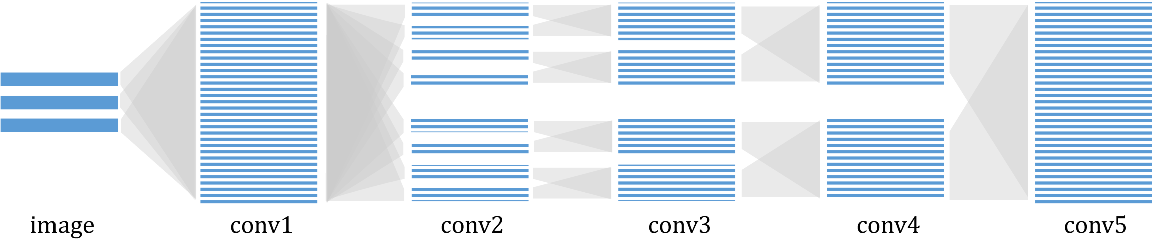
\includegraphics[width=\columnwidth, page=1]{networktopology}
			\caption{Root-8 topology}
			\label{fig:roottopology}
		\end{subfigure}
		~
		\begin{subfigure}[b]{0.85\columnwidth}
			\includegraphics[width=\columnwidth, page=2]{networktopology}
			\caption{Tree-2 topology}
			\label{fig:treetopology}
		\end{subfigure}
		~
		\begin{subfigure}[b]{0.85\columnwidth}
			\includegraphics[width=\columnwidth, page=3]{networktopology}
			\caption{Columnar-4 topology}
			\label{fig:columntopology}
		\end{subfigure}
		\caption[Filter group network topologies]{\textbf{Filter Group Network Topologies.} Topologies of filter groups explored, as illustrated in a VGG-style deep network. Grey blocks represent the input range over which a layer's filters operate, while coloured blocks represent the stacked feature maps of the filter groups within each layer. 
			%Root topologies assume that filters become more correlated with depth, while tree topologies assume filters become less correlated with depth.
		}
		\label{fig:networktopology}
	\end{figure}
	
	\subsubsection{Columns.} Columnar topologies assume that filters are consistently co-dependent with depth, and that this co-dependence is relatively small throughout the whole network. AlexNet uses a 2-column architecture on most layers.
	
	\subsubsection{Trees.} Tree-like topologies, as used by~\citet{Ioannou2016},  in conditional networks, assume that either filters become less co-dependent with depth, or the number of filters grows with depth enough that there are many more filters in deep layers than required. Notably,~\citet{Ioannou2016} evaluated their architecture on VGG networks, which are very large, and over-parametrized even compared to state-of-the-art networks such as residual networks.
	
	\subsubsection{Roots.} Root-like topologies (\ie inverted trees) assume that filters become more co-dependent with depth.  This aligns with the intuition of deep networks for image recognition subsuming the deformable parts model (DPM). If we assume that filter responses identify parts (or more elemental features), then there should be more filter co-dependence with depth, as more complex relationships emerge~\cite{girshick2015deformable}.
	
	In general, state-of-the-art CNN architectures have few filters in early convolutional layers, increasing throughout the network, and so it might seem that trees would have the best computational savings. Even so, the first few layers of a CNN are always the most computationally expensive, simply because the input feature map's spatial size is largest before any sub-sampling, in the layers close to the input image. As such, root topologies in general have the largest computational savings.
	
	%\subsection{Layer-wise Filter Covariance in Deep Networks}
	%We used the DeCov loss (see Eqn.~\ref{eqn:decov}) as a measure of the covariance of the filters on each convolutional layer. Although \citet{Cogswell2016} only use DeCov on fully-connected layers, we expanded it's use to convolutional layers by calculating the covariance of the average activation over each filter's feature map in a convolutional layer, rather than the activation of each neuron in a fully-connected layer. Instead of calculating batch statistics, the covariance and mean were calculated over a large random sample of training data.
	%\input{decovplot.tex}
	
	%\textit{Network in Network.}
	%For the NiN network, the DeCov loss was calculated over the entire CIFAR10 training set for a number of different model states from different training epochs, plotted on a log scale in Fig.~\ref{fig:decovplot_nincifar}. Even after a few training epochs the co-variance of filters in the first few layers is significantly reduced. The final network, after 300 epochs, shows a clear increase in co-variance with network depth, with layers close to the output layer having much higher covariance.
	
	%\textit{ResNet 50.}
	%Fig.~\ref{fig:decovplot} shows the per-layer DeCov loss for ResNet 50 plotted on a log scale. It was calculated over a 10000 random sub-sample of the ILSVRC training data for various training epochs. Clearly, filter covariance increases drastically with filter depth.
	
	%\textit{GoogLeNet.}
	%Fig.~\ref{fig:decovplot_googlenet} shows the per-layer DeCov loss for GoogLeNet plotted on a log scale, calculated over a 10000 random sub-sample of the ILSVRC training data. GoogLeNet is unusual in training with multiple intermediate losses. While each of the classifiers and fully-connected layers associated with the losses has high filter covariance, but the covariance of the composite responses of each of the inception units is relatively constant with depth, with the notable exception of `inception-4d'.
	
	%Given the results of our analysis of the layer-wise filter covariance in deep networks, we found filter covariance in deep networks be maintained or increase with depth. However, given that the number of filters per-layer increases rapidly with depth in all of these networks, on a per-filter basis, covariance is increasing. Given this, a root topology fits these findings best. 
	
	\section{Results}
	%Our approach is to explicitly separate convolutions within a network into many individual filter groups, similar to the approach of \citet{Ioannou2016}. However, instead of a tree-like topology, we propose that filters responses become more co-dependent with depth rather than less, and so a root-like topology is more appropriate.
	Here we present results of training from scratch re-structured (as described in \S\ref{method}) state-of-the-art network architectures for image classification on the CIFAR-10~\cite{CIFAR10} and ILSVRC~\citep{ILSVRC2015} datasets.
	
	\subsection{Improving Network in Network on CIFAR-10}
	Network in Network (NiN)~\cite{Lin2014} is a near state-of-the-art network for CIFAR-10~\cite{CIFAR10}. It is composed of 3 spatial (5$\times$5, 3$\times$3) convolutional layers with a large number of filters (192), interspersed with low-dimensional embedding (1$\times$1) layers. We replicated the standard NiN network architecture as described by \citet{Lin2014}, but with state-of-the-art training methods. We trained using random 32$\times$32 cropped and mirrored images from 4-pixel zero-padded  mean-subtracted images, as in~\citep{goodfellow2013maxout, He2015}. We also used the initialization of \citet{He2015b} and batch normalization~\citep{Ioffe2015}. With this configuration, ZCA whitening was not required to reproduce validation accuracies obtained in~\citep{Lin2014}. We also did not use dropout, having found it to have little effect, presumably due to our use of batch normalization.

	\begin{table}[tbp]
		\caption[Network-in-Network CIFAR10 root results]{\textbf{Network-in-Network CIFAR10}}
		\label{table:nincifarresults}
		\centering
		%\resizebox{\columnwidth}{!}{
		\pgfplotstableread[col sep=comma]{rootdata/nincifarbest.csv}\data
		
		\pgfplotstabletypeset[
		every head row/.style={
			before row=\toprule,after row=\midrule},
		every last row/.style={
			after row=\bottomrule},
		every first row/.style={
			after row=\bottomrule}, 
		fixed zerofill,     % Fill numbers with zeros
		columns={name, ma, param, accuracy, cpu, gpu},
		columns/name/.style={
			column name=Model,
			string type
		},
		columns/ma/.style={
			column name=FLOPS {\small $\times 10^{8}$},
			preproc/expr={{##1/1e8}}
		},
		columns/param/.style={
			column name=Param. {\small $\times 10^{5}$},
			preproc/expr={{##1/1e5}}
		},
		column type/.add={lrrrrrr}{},
		columns/accuracy/.style={
			column name=Accuracy,
			precision=4
		},
		columns/gpu/.style={
			column name=GPU (ms),
			precision=3
		},
		columns/cpu/.style={
			column name=CPU (ms),
			precision=1
		},
		highlight col max ={\data}{accuracy},
		highlight col min ={\data}{param}, 
		highlight col min ={\data}{ma}, 
		col sep=comma]{\data}
		%}
	\end{table}
	
	We restructured the network with hierarchical groups, while preserving the original number of filters per layer. To determine which of the network topologies in Fig.~\ref{fig:networktopology} gave the best computational savings with the minimal loss in accuracy, we implemented each for various numbers of initial filter groups.
	
	We only group filters within the the spatial (\ie non 1$\times$1) layers. Using filter groups within the low-dimensional embedding layers (\ie 1$\times$1 convolutions) leads to learning even lower dimensional embeddings of the input space, which is likely to compromise their representational ability. Indeed, in such configurations we observed a large decrease in accuracy. We also do not group filters in the first convolutional layer -- since it operates on the three-channel image space, it is of limited computational impact compared to other layers, and we believe learning color filters to be critical to learning. 
	
	Table~\ref{table:nincifarresults} lists the best results for each of the topologies.
	% (also plotted in Fig.~\ref{fig:nincifarplotsconvonly}).
	Only the root-like topology maintains accuracy while decreasing computation and model size significantly -- the best, root-4, has only 55\% of the floating point operations (FLOPS), 47\% of the model parameters of the original network, and approximately 22\% faster CPU and GPU timings.
	
	\begin{figure}[tbp]
		\centering
		\begin{subfigure}[b]{0.95\columnwidth}
			\pgfplotstableread[col sep=comma]{rootdata/nincifar.csv}\datatable
			\pgfplotstableread[col sep=comma]{rootdata/nincifar_root_s.csv}\rdatatable
			%\pgfplotstableread[col sep=comma]{rootdata/nincifar_col_s.csv}\cdatatable
			\pgfplotstableread[col sep=comma]{rootdata/nincifar_tree_s.csv}\tdatatable
			\pgfplotsset{major grid style={dotted,red}}
			
			\centering
			\begin{tikzpicture}
			%tikzstyle{every node}=[font=\scriptsize]
			\begin{axis}[
			width=\columnwidth,
			height=0.66\columnwidth,
			axis x line=bottom,
			ylabel=Error,
			xlabel=Model Parameters,
			axis lines=left,
			enlarge x limits=0.05,
			enlarge y limits=0.2,
			grid=major,
			%xmin=0,
			%ytick={0.01,0.02,...,0.2},
			%ymin=0.075,ymax=0.09,
			xticklabel style={
				/pgf/number format/fixed,
				/pgf/number format/precision=3
			},
			yticklabel={\pgfmathparse{\tick*1}\pgfmathprintnumber{\pgfmathresult}\%},style={
				/pgf/number format/fixed,
				/pgf/number format/precision=1
			},
			legend style={at={(1,1.1)}, anchor=south east, column sep=0.2em, font=\small},
			legend columns=4,
			]
			\addplot[mark=*,mark options={fill=red},
			%nodes near coords,
			only marks,
			point meta=explicit symbolic,
			] table[meta=name,x=param,y expr={1 - \thisrow{accuracy} },]{\datatable};
			\addplot[mark=square*,mark options={fill=green},
			nodes near coords, only marks,
			every node near coord/.append style={inner sep=4pt},
			point meta=explicit symbolic,
			] table[meta=name,x=param,y expr={1 - \thisrow{accuracy} },]{\rdatatable};
			%\addplot[mark=triangle*,mark options={fill=blue},
			%   nodes near coords, nodes near coords align = {above}, only marks,
			%   every node near coord/.append style={inner sep=4pt},
			%   only marks,
			%   point meta=explicit symbolic,
			%] table[meta=name,x=param,y expr={1 - \thisrow{accuracy} },]{\cdatatable};
			\addplot[mark=diamond*,mark options={fill=magenta},
			nodes near coords, nodes near coords align = {below}, only marks,
			every node near coord/.append style={inner sep=4pt},
			only marks,
			point meta=explicit symbolic,
			] table[meta=name,x=param,y expr={1 - \thisrow{accuracy} },]{\tdatatable};
			
			\legend{NiN, Root, Tree}
			\end{axis}
			\end{tikzpicture}
			\caption{\textbf{Model Parameters \vs Error.}}
			%\label{fig:nincifarparamconvonly}
		\end{subfigure}
		\begin{subfigure}[b]{0.95\columnwidth}
			\pgfplotstableread[col sep=comma]{rootdata/nincifar.csv}\datatable
			\pgfplotstableread[col sep=comma]{rootdata/nincifar_root_s.csv}\rdatatable
			%\pgfplotstableread[col sep=comma]{rootdata/nincifar_col_s.csv}\cdatatable
			\pgfplotstableread[col sep=comma]{rootdata/nincifar_tree_s.csv}\tdatatable
			\pgfplotsset{major grid style={dotted,red}}
			
			\centering
			\begin{tikzpicture}
			%tikzstyle{every node}=[font=\scriptsize]
			\begin{axis}[
			width=\columnwidth,
			height=0.66\columnwidth,
			axis x line=bottom,
			ylabel=Error,
			xlabel=FLOPS (Multiply-Add),
			axis lines=left,
			enlarge x limits=0.05,
			enlarge y limits=0.2,
			grid=major,
			%xmin=0,
			%ytick={0.01,0.02,...,0.2},
			%ymin=0.075,ymax=0.09,
			xticklabel style={
				/pgf/number format/fixed,
				/pgf/number format/precision=3
			},
			yticklabel={\pgfmathparse{\tick*1}\pgfmathprintnumber{\pgfmathresult}\%},style={
				/pgf/number format/fixed,
				/pgf/number format/precision=1
			},
			legend style={at={(1,1.1)}, anchor=south east, column sep=0.2em, font=\small},
			legend columns=4,
			]
			\addplot[mark=*,mark options={fill=red},
			%nodes near coords,
			only marks,
			point meta=explicit symbolic,
			] table[meta=name,x=ma,y expr={1 - \thisrow{accuracy} },]{\datatable};
			\addplot[mark=square*,mark options={fill=green},
			nodes near coords, only marks,
			every node near coord/.append style={inner sep=4pt},
			point meta=explicit symbolic,
			] table[meta=name,x=ma,y expr={1 - \thisrow{accuracy} },]{\rdatatable};
			%\addplot[mark=triangle*,mark options={fill=blue},
			%   nodes near coords, nodes near coords align = {above}, only marks,
			%   every node near coord/.append style={inner sep=4pt},
			%   only marks,
			%   point meta=explicit symbolic,
			%] table[meta=name,x=ma,y expr={1 - \thisrow{accuracy} },]{\cdatatable};
			\addplot[mark=diamond*,mark options={fill=magenta},
			nodes near coords, nodes near coords align = {below}, only marks,
			every node near coord/.append style={inner sep=4pt},
			only marks,
			point meta=explicit symbolic,
			] table[meta=name,x=ma,y expr={1 - \thisrow{accuracy} },]{\tdatatable};
			%\legend{NiN, Root, Column, Tree}
			\end{axis}
			\end{tikzpicture}
			\caption{\textbf{FLOPS (Multiply-Add) \vs Error.}}
			%\label{fig:nincifarmaconvonly}
		\end{subfigure}
		
		\caption[Network-in-Network CIFAR10 root results]{\textbf{Network-in-Network CIFAR10.} Spatial filters (3$\times$3, 5$\times$5) are grouped hierarchically. Root topologies maintain accuracy better as compared to 
			%column or
			tree topologies. The best models are closest to the origin.
			%(left) Parameters \vs Error, (right) FLOPS \vs Error.
		}
		\label{fig:nincifarplotsconvonly}
	\end{figure}
	
	\subsection{Improving Residual Networks on ILSVRC}
	Residual networks (ResNets)~\citep{He2015} are the state-of-the art network for ILSVRC. ResNets are more computationally efficient than the VGG architecture~\cite{Simonyan2014verydeep} they are based on, due to the use of so called `bottleneck' layers (low-dimensional embeddings~\citep{Lin2014}), but are also more accurate and quicker to converge, due to the use of identity mappings (shortcuts). These shortcut connections have been shown to help the training of deep networks. 
	
	\subsubsection{ResNet 50}
	\label{resnet50results}
	We chose to apply root filter hierarchies within the `ResNet 50' model~\citep{He2015}, the largest residual network model to fit onto 8 GPUs. ResNet 50 has 50 convolutional layers, of which one-third are spatial convolutions (non-1$\times$1). We did not use any training augmentation aside from random cropping and mirroring. 
	To aid training, we used the initialization of \citep{He2015b} but modified for compound layers~\citep{Ioannou2016}, and batch normalization~\citep{Ioffe2015}.
\begin{table}[tbp]
	\caption[ResNet 50 ILSVRC root results]{\textbf{ResNet 50 ILSVRC}}
	\label{table:resnet50imagenetresults}
	%\resizebox{\columnwidth}{!}{
	\tabcolsep=5pt
	\centering
	\pgfplotstableread[col sep=comma]{rootdata/resnet50ma.csv}\data
	%\pgfplotstableread[col sep=comma]{rootdata/resnet50maall.csv}\alldata
	\pgfplotstableread[col sep=comma]{rootdata/resnet50maconvonly.csv}\codata
	%\pgfplotstablevertcat{\data}{\alldata}
	\pgfplotstablevertcat{\data}{\codata}
	\pgfplotstableset{
		create on use/singlegpu/.style={
			create col/expr={\thisrow{GPU Forward} / \thisrow{Batch Size}}},
	}
	\pgfplotstableset{
		create on use/singlecpu/.style={
			create col/expr={\thisrow{CPU Forward} / \thisrow{Batch Size}}},
	}
	\pgfplotstabletypeset[
	every head row/.style={
		before row=\toprule,after row=\midrule},
	every last row/.style={
		after row=\bottomrule},
	every first row/.style={
		after row=\bottomrule}, 
	fixed zerofill,     % Fill numbers with zeros
	columns={Full Name, Multiply-Acc., Param., Top-1 Acc., Top-5 Acc., singlecpu, singlegpu},
	columns/Full Name/.style={
		column name=Root,
		string type
	},
	columns/singlegpu/.style={
		column name=GPU (ms),
		precision=1
	},
	columns/singlecpu/.style={
		column name=CPU (ms),
		precision=0
	},
	columns/Multiply-Acc./.style={
		column name=FLOPS {\small $\times 10^{9}$},
		preproc/expr={{##1/1e9}}
	},
	columns/Param./.style={
		column name=Param. {\small $\times 10^{7}$},
		preproc/expr={{##1/1e7}}
	},
	column type/.add={lrrrrrr}{},
	columns/Top-1 Acc./.style={precision=3},
	columns/Top-5 Acc./.style={precision=3},
	highlight col max ={\data}{Top-1 Acc.},
	highlight col max ={\data}{Top-5 Acc.}, 
	highlight col min ={\data}{Param.}, 
	highlight col min ={\data}{Multiply-Acc.}, 
	col sep=comma]{\data}
	%}
\end{table}
	
	\begin{table}[tb]
		\caption[ResNet 50 ILSVRC root results]{\textbf{ResNet 50}. Filter groups in each convolutional layer.}
		\label{table:resnet50config}
		\centering
		\tabcolsep=5pt
		%\resizebox{\columnwidth}{!}{
		\begin{tabular}{lcccccccccccc}
			\toprule
			\textbf{Root} & \textbf{conv1} & \multicolumn{2}{c}{\textbf{res2\{a--c\}}} & \multicolumn{2}{c}{\textbf{res3\{a--d\}}} & \multicolumn{2}{c}{\textbf{res4\{a--f\}}} & \multicolumn{2}{c}{\textbf{res5\{a--c\}}} \\
			& \textit{7$\times$7} & \textit{1$\times$1} & \textit{3$\times$3} & \textit{1$\times$1} & \textit{3$\times$3} & \textit{1$\times$1} & \textit{3$\times$3} & \textit{1$\times$1} & \textit{3$\times$3} \\
			%    \midrule
			%    2 & 1 & 2 & 2 & 1 & 1 & 1 & 1 & 1 & 1 \\
			%    4 & 1 & 4 & 4 & 2 & 2 & 1 & 1 & 1 & 1 \\
			%    8 & 1 & 8 & 8 & 4 & 4 & 2 & 2 & 1 & 1 \\
			%    \midrule
			4 (s)& 1 & 1 & 4 & 1 &  2 & 1 &  1 & 1 & 1 \\
			8 (s) & 1 & 1 & 8 & 1 &  4 & 1 &  2 & 1 & 1 \\
			16 (s) & 1 & 1 & 16 & 1 &  8 & 1 &  4 & 1 & 2 \\
			32 (s) & 1 & 1 & 32 & 1 & 16 & 1 &  8 & 1 & 4 \\
			64 (s) & 1 & 1 & 64 & 1 & 32 & 1 & 16 & 1 & 8 \\
			\bottomrule
		\end{tabular}
		%}
	\end{table}
	While preserving the original number of filters per layer, networks with various numbers of filter groups were trained in a root topology, as described in Table~\ref{table:resnet50config}. We only grouped filters within each of the `spatial' convolutions (3$\times$3), denoted \textbf{(s)} in Table \ref{table:resnet50imagenetresults}. For all layers between sub-sampling layers, we split the filters into the same number of groups, for example a ResNet 50 model with a root-8 topology has eight groups of filters on layers \texttt{res2\{a,b,c\}}, four on layers \texttt{res3\{a,\ldots, d\}}, two on layers \texttt{res4\{a,\ldots,f\}} and a single group on all other convolutional layers.
	
	As shown in Fig.~\ref{fig:resnet50plots}, our method yields a significant reduction in computational complexity -- as measured in FLOPS (multiply-adds), CPU and GPU timings -- and model size, as measured in the number of floating point parameters. All timings were taken on the network's forward pass, using Caffe compiled with the CuDNN and MKL BLAS libraries, on a machine with an Nvidia Titan Z GPU and 2 10-core Intel Xeon E5-2680 v2 CPUs. We do not factor the batch normalization layers into our FLOPS or parameter counts since, as argued by~\citet{Szegedy2014going}, at test time the batch normalization layers/parameters may effectively be removed.
	
	For many of the configurations the accuracy is 0.2\% higher than that of the baseline network. Of these, the best result (root-16) exceeds the baseline accuracy by 0.2\% while reducing the model size by 27\% and floating-point operations (multiply-add) by 37\%. CPU timings were 23\% faster, while GPU timings were 13\% faster\footnote{See \S\ref{gpuexplanation} for an explanation of the GPU timing disparity.}. With a drop in accuracy of only 0.1\% however, the root-64 model reduces the model size by 40\%, and reduces the floating point operations by 45\%. CPU timings were 31\% faster, while GPU timings were 12\% faster. 
	
\begin{figure}[tbp]
	\centering
	\begin{subfigure}[b]{0.95\columnwidth}
		\pgfplotstableread[col sep=comma]{rootdata/resnet50ma.csv}\gdatatable
		\pgfplotstableread[col sep=comma]{rootdata/resnet50maall.csv}\alldatatable
		\pgfplotstableread[col sep=comma]{rootdata/resnet50maconvonly.csv}\codatatable
		\pgfplotsset{major grid style={dotted,red}}
		
		\pgfplotstableset{
			create on use/singlecpu/.style={
				create col/expr={\thisrow{CPU Forward} / \thisrow{Batch Size}}},
		}
		
		\centering
		\begin{tikzpicture}
		\begin{axis}[
		width=\columnwidth,
		height=0.33\columnwidth,
		axis x line=bottom,
		ylabel=Top-5 Error,
		xlabel=Model Parameters (\# Floats),
		axis lines=left,
		enlarge x limits=0.10,
		enlarge y limits=0.1,
		grid=major,
		%xmin=0,
		ytick={0.01,0.02,...,0.2},
		ymin=0.07,ymax=0.13,
		xticklabel style={
			/pgf/number format/fixed,
			/pgf/number format/precision=3
		},
		yticklabel={\pgfmathparse{\tick*100}\pgfmathprintnumber{\pgfmathresult}\%},style={
			/pgf/number format/fixed,
			/pgf/number format/precision=1
		},
		legend style={at={(0.98,0.98)}, anchor=north east, column sep=0.5em},
		legend columns=3,
		]
		\addplot[mark=*,mark options={fill=red},
		%nodes near coords,
		only marks,
		point meta=explicit symbolic,
		] table[meta=Network,x=Param.,y expr={1 - \thisrow{Top-5 Acc.} },]{\gdatatable};
		\addplot[mark=square*,mark options={fill=green},
		nodes near coords, only marks,
		every node near coord/.append style={inner sep=4pt},
		point meta=explicit symbolic,
		] table[meta=Network,x=Param.,y expr={1 - \thisrow{Top-5 Acc.} },]{\alldatatable};
		\addplot[mark=triangle*,mark options={fill=blue},
		nodes near coords, nodes near coords align = {below}, only marks,
		every node near coord/.append style={inner sep=4pt},
		only marks,
		point meta=explicit symbolic,
		] table[meta=Network,x=Param.,y expr={1 - \thisrow{Top-5 Acc.} },]{\codatatable};
		\legend{ResNet 50, All Filters, Spatial Filters, LDE Half}
		\end{axis}
		\end{tikzpicture}
		\caption{\textbf{Model Parameters \vs Top-5 Error.}}
		\label{fig:resnet5050param}
	\end{subfigure}
	~
	\begin{subfigure}[b]{0.95\columnwidth}
		\pgfplotstableread[col sep=comma]{rootdata/resnet50ma.csv}\gdatatable
		\pgfplotstableread[col sep=comma]{rootdata/resnet50maall.csv}\alldatatable
		\pgfplotstableread[col sep=comma]{rootdata/resnet50maconvonly.csv}\codatatable
		\pgfplotstableread[col sep=comma]{rootdata/resnet50maconvhalf.csv}\hdatatable
		\pgfplotsset{major grid style={dotted,red}}
		
		\centering
		\begin{tikzpicture}
		\begin{axis}[
		width=\columnwidth,
		height=0.33\columnwidth,
		axis x line=bottom,
		ylabel=Top-5 Error,
		xlabel=FLOPS (Multiply-Add),
		axis lines=left,
		enlarge x limits=0.10,
		enlarge y limits=0.1,
		grid=major,
		%xmin=0,
		ytick={0.01,0.02,...,0.2},
		ymin=0.07,ymax=0.13,
		xticklabel style={
			/pgf/number format/fixed,
			/pgf/number format/precision=3
		},
		yticklabel={\pgfmathparse{\tick*100}\pgfmathprintnumber{\pgfmathresult}\%},style={
			/pgf/number format/fixed,
			/pgf/number format/precision=1
		},
		legend style={at={(0.98,0.98)}, anchor=north east, column sep=0.5em},
		legend columns=3,
		]
		\addplot[mark=*,mark options={fill=red},
		%nodes near coords,
		only marks,
		point meta=explicit symbolic,
		] table[meta=Network,x=Multiply-Acc.,y expr={1 - \thisrow{Top-5 Acc.} },]{\gdatatable};
		\addplot[mark=square*,mark options={fill=green},
		nodes near coords, only marks,
		every node near coord/.append style={inner sep=4pt},
		point meta=explicit symbolic,
		] table[meta=Network,x=Multiply-Acc.,y expr={1 - \thisrow{Top-5 Acc.} },]{\alldatatable};
		\addplot[mark=triangle*,mark options={fill=blue},
		nodes near coords, nodes near coords align = {below}, only marks,
		every node near coord/.append style={inner sep=4pt},
		only marks,
		point meta=explicit symbolic,
		] table[meta=Network,x=Multiply-Acc.,y expr={1 - \thisrow{Top-5 Acc.} },]{\codatatable};
		\end{axis}
		\end{tikzpicture}
		\caption{\textbf{FLOPS (Multiply-Add) \vs Top-5 Error.}}
		\label{fig:resnet50ma}
	\end{subfigure}
	~
	\begin{subfigure}[b]{0.95\columnwidth}
		\pgfplotstableread[col sep=comma]{rootdata/resnet50ma.csv}\gdatatable
		\pgfplotstableread[col sep=comma]{rootdata/resnet50maall.csv}\alldatatable
		\pgfplotstableread[col sep=comma]{rootdata/resnet50maconvonly.csv}\codatatable
		\pgfplotstableread[col sep=comma]{rootdata/resnet50maconvhalf.csv}\hdatatable
		\pgfplotsset{major grid style={dotted,red}}
		
		\centering
		\begin{tikzpicture}
		\begin{axis}[
		width=\columnwidth,
		height=0.33\columnwidth,
		axis x line=bottom,
		ylabel=Top-5 Error,
		xlabel=GPU Forward (ms),
		axis lines=left,
		enlarge x limits=0.10,
		enlarge y limits=0.1,
		grid=major,
		%xmin=0,
		ytick={0.01,0.02,...,0.2},
		ymin=0.07,ymax=0.13,
		xticklabel style={
			/pgf/number format/fixed,
			/pgf/number format/precision=3
		},
		yticklabel={\pgfmathparse{\tick*100}\pgfmathprintnumber{\pgfmathresult}\%},style={
			/pgf/number format/fixed,
			/pgf/number format/precision=1
		},
		legend style={at={(0.98,0.98)}, anchor=north east, column sep=0.5em},
		legend columns=3,
		]
		\addplot[mark=*,mark options={fill=red},
		%nodes near coords,
		only marks,
		point meta=explicit symbolic,
		] table[meta=Network,
		x expr={\thisrow{GPU Forward} / \thisrow{Batch Size}},
		y expr={1 - \thisrow{Top-5 Acc.} }
		]{\gdatatable};
		\addplot[mark=square*,mark options={fill=green},
		nodes near coords, only marks,
		every node near coord/.append style={inner sep=4pt},
		point meta=explicit symbolic,
		] table[meta=Network,
		x expr={\thisrow{GPU Forward} / \thisrow{Batch Size}},
		y expr={1 - \thisrow{Top-5 Acc.} },
		]{\alldatatable};
		\addplot[mark=triangle*,mark options={fill=blue},
		nodes near coords, nodes near coords align = {below}, only marks,
		every node near coord/.append style={inner sep=4pt},
		only marks,
		point meta=explicit symbolic,
		] table[meta=Network,
		x expr={\thisrow{GPU Forward} / \thisrow{Batch Size}},
		y expr={1 - \thisrow{Top-5 Acc.} },
		]{\codatatable};
		%\legend{ResNet 50, All Filters, Spatial Filters}
		\end{axis}
		\end{tikzpicture}
		\caption{\textbf{GPU Forward Time \vs Top-5 Error.}}
		\label{fig:resnet5050gpuforward}
	\end{subfigure}
	~
	\begin{subfigure}[b]{0.95\columnwidth}
		\pgfplotstableread[col sep=comma]{rootdata/resnet50ma.csv}\gdatatable
		\pgfplotstableread[col sep=comma]{rootdata/resnet50maall.csv}\alldatatable
		\pgfplotstableread[col sep=comma]{rootdata/resnet50maconvonly.csv}\codatatable
		\pgfplotstableread[col sep=comma]{rootdata/resnet50maconvhalf.csv}\hdatatable
		\pgfplotsset{major grid style={dotted,red}}
		
		\centering
		\begin{tikzpicture}
		\begin{axis}[
		width=\columnwidth,
		height=0.33\columnwidth,
		axis x line=bottom,
		ylabel=Top-5 Error,
		xlabel=CPU Forward (ms),
		axis lines=left,
		enlarge x limits=0.10,
		enlarge y limits=0.1,
		grid=major,
		%xmin=0,
		ytick={0.01,0.02,...,0.2},
		ymin=0.07,ymax=0.13,
		xticklabel style={
			/pgf/number format/fixed,
			/pgf/number format/precision=3
		},
		yticklabel={\pgfmathparse{\tick*100}\pgfmathprintnumber{\pgfmathresult}\%},style={
			/pgf/number format/fixed,
			/pgf/number format/precision=1
		},
		legend style={at={(0.98,0.98)}, anchor=north east, column sep=0.5em},
		legend columns=3,
		]
		\addplot[mark=*,mark options={fill=red},
		%nodes near coords,
		only marks,
		point meta=explicit symbolic,
		] table[meta=Network,
		x expr={\thisrow{CPU Forward} / \thisrow{Batch Size}},
		y expr={1 - \thisrow{Top-5 Acc.} },
		]{\gdatatable};
		\addplot[mark=square*,mark options={fill=green},
		nodes near coords, only marks,
		every node near coord/.append style={inner sep=4pt},
		point meta=explicit symbolic,
		] table[meta=Network,
		x expr={\thisrow{CPU Forward} / \thisrow{Batch Size}},
		y expr={1 - \thisrow{Top-5 Acc.} },
		]{\alldatatable};
		\addplot[mark=triangle*,mark options={fill=blue},
		nodes near coords, nodes near coords align = {below}, only marks,
		every node near coord/.append style={inner sep=4pt},
		only marks,
		point meta=explicit symbolic,
		] table[meta=Network,
		x expr={\thisrow{CPU Forward} / \thisrow{Batch Size}},
		y expr={1 - \thisrow{Top-5 Acc.} },
		]{\codatatable};
		%\legend{ResNet 50, All Filters, Spatial Filters}
		\end{axis}
		\end{tikzpicture}
		\caption{\textbf{CPU Forward Time \vs Top-5 Error.}}
		\label{fig:resnet5050cpuforward}
	\end{subfigure}
	
	\caption[ResNet 50 ILSVRC root results]{\textbf{ResNet 50.} Models with filter groups have fewer parameters, and less floating point operations, while maintaining error comparable to the baseline.}
	\label{fig:resnet50plots}
\end{figure}
	
	\subsubsection{ResNet 200}
	\label{resnet200results}
	\begin{table}[tbp]
		\caption[ResNet 200 ILSVRC root results]{\textbf{ResNet 200 ILSVRC}}
		\label{table:resnet200imagenetresults}
		%\resizebox{\columnwidth}{!}{
		\centering
		\pgfplotstableread[col sep=comma]{rootdata/resnet200.csv}\data
		\pgfplotstabletypeset[
		every head row/.style={
			before row=\toprule,after row=\midrule},
		every last row/.style={
			after row=\bottomrule},
		every first row/.style={
			after row=\bottomrule}, 
		fixed zerofill,     % Fill numbers with zeros
		columns={name, ma, param, top1, top5},
		columns/name/.style={
			column name=Root,
			string type
		},
		columns/ma/.style={
			column name=FLOPS {\small $\times 10^{12}$},
			preproc/expr={{##1/1e12}}
		},
		columns/param/.style={
			column name=Param. {\small $\times 10^{7}$},
			preproc/expr={{##1/1e7}}
		},
		column type/.add={lrrrrrr}{},
		columns/top1/.style={
			precision=3,
			column name=Top-1 Error,
		},
		columns/top5/.style={
			precision=3,
			column name=Top-5 Error,
		},
		highlight col min ={\data}{top1},
		highlight col min ={\data}{top5}, 
		highlight col min ={\data}{param}, 
		highlight col min ={\data}{ma}, 
		col sep=comma]{\data}
		%}
	\end{table}
	To show that the method applies to deeper architectures, we also applied our method to ResNet 200, the deepest network for ILSVRC 2012. For this network we used code implementing full training augmentation to achieve state-of-the-art results\footnote{\url{https://github.com/facebook/fb.resnet.torch}}, re-implementing more recent models~\citep{He2016}. Table \ref{table:resnet200imagenetresults} shows the results of these experiments, top-1 and top-5 error are for center cropped images. The models trained with hierarchical filter groups have comparable error to the baseline network, with fewer parameters and less computation. The root-32 model has 25\% fewer FLOPS and 44\% fewer parameters than ResNet 200.
\begin{figure}[tbp]
	\centering
	\begin{subfigure}[b]{0.95\textwidth}
		\pgfplotstableread[col sep=comma]{rootdata/resnet200.csv}\datatable
		\pgfplotsset{major grid style={dotted,red}}
		
		\centering
		\begin{tikzpicture}
		\begin{axis}[
		width=\columnwidth,
		height=0.33\columnwidth,
		axis x line=bottom,
		ylabel=Top-5 Error,
		xlabel=Model Parameters (\# Floats),
		axis lines=left,
		enlarge x limits=0.10,
		enlarge y limits=0.1,
		grid=major,
		%xmin=0,
		ytick={0,1,2,...,10},
		ymin=5,ymax=10,
		xticklabel style={
			/pgf/number format/fixed,
			/pgf/number format/precision=3
		},
		yticklabel={\pgfmathparse{\tick}\pgfmathprintnumber{\pgfmathresult}\%},style={
			/pgf/number format/fixed,
			/pgf/number format/precision=1
		},
		legend style={at={(0.98,0.98)}, anchor=north east, column sep=0.5em},
		legend columns=3,
		]
		\addplot[mark=*,mark options={fill=red},
		nodes near coords, only marks,
		every node near coord/.append style={inner sep=4pt},
		only marks,
		point meta=explicit symbolic,
		] table[meta=name,x=param,y=top5,]{\datatable};
		\end{axis}
		\end{tikzpicture}
		\caption{\textbf{Model Parameters \vs Top-5 Error.}}
		\label{fig:resnet200param}
	\end{subfigure}
	~
	\begin{subfigure}[b]{0.95\textwidth}
		\pgfplotstableread[col sep=comma]{rootdata/resnet200.csv}\datatable
		\pgfplotsset{major grid style={dotted,red}}
		
		\centering
		\begin{tikzpicture}
		\begin{axis}[
		width=\columnwidth,
		height=0.33\columnwidth,
		axis x line=bottom,
		ylabel=Top-5 Error,
		xlabel=Model Parameters (\# Floats),
		axis lines=left,
		enlarge x limits=0.10,
		enlarge y limits=0.1,
		grid=major,
		%xmin=0,
		ytick={0,1,2,...,10},
		ymin=5,ymax=10,
		xticklabel style={
			/pgf/number format/fixed,
			/pgf/number format/precision=3
		},
		yticklabel={\pgfmathparse{\tick}\pgfmathprintnumber{\pgfmathresult}\%},style={
			/pgf/number format/fixed,
			/pgf/number format/precision=1
		},
		legend style={at={(0.98,0.98)}, anchor=north east, column sep=0.5em},
		legend columns=3,
		]
		\addplot[mark=*,mark options={fill=red},
		nodes near coords, only marks,
		every node near coord/.append style={inner sep=4pt},
		only marks,
		point meta=explicit symbolic,
		] table[meta=name,x=ma,y=top5,]{\datatable};
		\end{axis}
		\end{tikzpicture}
		\caption{\textbf{FLOPS \vs Top-5 Error.}}
		\label{fig:resnet200ma}
	\end{subfigure}
	
	\caption[ResNet 200 ILSVRC root results]{\textbf{ResNet 200 ILSVRC.} Models with filter groups have fewer parameters, and less floating point operations, while maintaining error comparable to the baseline.}
	\label{fig:resnet200plots}
\end{figure}
	
	\subsection{Improving GoogLeNet on ILSVRC}
	\label{googlenet50results}
	
	\begin{table}[tbp]
		\caption[GoogLeNet ILSVRC root results]{\textbf{GoogLeNet ILSVRC}}
		\label{table:googlenetimagenetresults}
		%\resizebox{\columnwidth}{!}{
		\tabcolsep=5pt
		\centering
		\pgfplotstableread[col sep=comma]{rootdata/googlenetma.csv}\data
		\pgfplotstableread[col sep=comma]{rootdata/googlenetmaall.csv}\alldata
		\pgfplotstableread[col sep=comma]{rootdata/googlenetmaconvonly.csv}\codata
		\pgfplotstablevertcat{\data}{\alldata}
		\pgfplotstablevertcat{\data}{\codata}
		\pgfplotstableset{
			create on use/singlegpu/.style={
				create col/expr={\thisrow{GPU Forward} / \thisrow{Batch Size}}},
		}
		\pgfplotstableset{
			create on use/singlecpu/.style={
				create col/expr={\thisrow{CPU Forward} / \thisrow{Batch Size}}},
		}
		\pgfplotstabletypeset[
		every head row/.style={
			before row=\toprule,after row=\midrule},
		every last row/.style={
			after row=\bottomrule},
		every first row/.style={
			after row=\bottomrule}, 
		fixed zerofill,     % Fill numbers with zeros
		columns={Full Name, Multiply-Acc., Param., Top-1 Acc., Top-5 Acc., singlecpu, singlegpu},
		columns/Full Name/.style={
			column name=Root,
			string type
		},
		columns/singlegpu/.style={
			column name=GPU (ms),
			precision=2
		},
		columns/singlecpu/.style={
			column name=CPU (ms),
			precision=0
		},
		columns/Multiply-Acc./.style={
			column name=FLOPS {\small $\times 10^{9}$},
			preproc/expr={{##1/1e9}}
		},
		columns/Param./.style={
			column name=Param. {\small $\times 10^{7}$},
			preproc/expr={{##1/1e7}}
		},
		columns/Top-1 Acc./.style={precision=3},
		columns/Top-5 Acc./.style={precision=3},
		highlight col max ={\data}{Top-1 Acc.},
		highlight col max ={\data}{Top-5 Acc.}, 
		highlight col min ={\data}{Param.}, 
		highlight col min ={\data}{Multiply-Acc.}, 
		column type/.add={lrrrrrr}{},
		col sep=comma]{\data}
		%}
	\end{table}
	
	
	\begin{table}[tb]
		\caption[GoogLeNet root architectures]{\textbf{GoogLeNet}. Filter groups in each convolutional layer.}
		\label{table:googlenetconfig}
		\centering
		\tabcolsep=5pt
		%\resizebox{\columnwidth}{!}{
		\begin{tabular}{lcccccccccccc}
			\toprule
			\textbf{Root} & \textbf{conv1} & \multicolumn{2}{c}{\textbf{conv2}} & \multicolumn{3}{c}{\textbf{inception3\{a,b\}}} & \multicolumn{3}{c}{\textbf{inception4\{a--e\}}} & \multicolumn{3}{c}{\textbf{inception5\{a,b\}}} \\
			& \textit{7$\times$7} & \textit{1$\times$1} & \textit{3$\times$3} & \textit{1$\times$1} & \textit{3$\times$3} & \textit{5$\times$5} & \textit{1$\times$1} & \textit{3$\times$3} & \textit{5$\times$5} & \textit{1$\times$1} & \textit{3$\times$3} & \textit{5$\times$5} \\
			\midrule
			2  & 1 &  2 &  2 & 1 & 1 & 1 & 1 & 1 & 1 & 1 & 1 & 1\\
			%    4  & 1 &  4 &  4 & 2 & 2 & 2 & 1 & 1 & 1 & 1 & 1 & 1\\
			8  & 1 &  8 &  8 & 4 & 4 & 4 & 2 & 2 & 2 & 1 & 1 & 1\\
			16 & 1 & 16 & 16 & 8 & 8 & 8 & 4 & 4 & 4 & 2 & 2 & 2\\
			\midrule
			2 (s)  & 1 &  1 &  2 & 1 & 1 & 1 & 1 & 1 & 1 & 1 & 1 & 1\\
			4 (s)  & 1 &  1 &  4 & 1 & 2 & 2 & 1 & 1 & 1 & 1 & 1 & 1\\
			8 (s)  & 1 &  1 &  8 & 1 & 4 & 4 & 1 & 2 & 2 & 1 & 1 & 1\\
			16 (s) & 1 &  1 & 16 & 1 & 8 & 8 & 1 & 4 & 4 & 1 & 2 & 2\\
			\bottomrule
		\end{tabular}
		%}
	\end{table}
	
	We replicated the network as described by~\citet{Szegedy2014going}, with the exception of not using any training augmentation aside from random crops and mirroring (as supported by Caffe~\cite{jia2014caffe}). To train we used the initialization of \citep{He2015b} modified for compound layers~\citep{Ioannou2016} and batch normalization without the scale and bias~\citep{Ioffe2015}. At test time we only evaluate the center crop image.
	
	While preserving the original number of filters per layer, we trained networks with various degrees of filter grouping, described in Table~\ref{table:googlenetconfig}.  While the inception architecture is relatively complex, for simplicity, we always use the same number of groups within each of the groups of different filter sizes, despite them having different cardinality. For some of the networks, we only grouped filters within each of the `spatial' convolutions (3$\times$3, 5$\times$5), denoted \textbf{(s)} in Table \ref{table:googlenetimagenetresults}. For other networks, we grouped all filters, including the 1$\times$1.

\begin{figure}[tbp]
	\centering
	\begin{subfigure}[b]{\columnwidth}
		\pgfplotstableread[col sep=comma]{rootdata/googlenetma.csv}\gdatatable
		\pgfplotstableread[col sep=comma]{rootdata/googlenetmaall.csv}\alldatatable
		\pgfplotstableread[col sep=comma]{rootdata/googlenetmaconvonly.csv}\codatatable
		\pgfplotsset{major grid style={dotted,red}}
		
		\centering
		\begin{tikzpicture}
		\begin{axis}[
		width=\columnwidth,
		height=0.33\columnwidth,
		axis x line=bottom,
		ylabel=Top-5 Error,
		xlabel=Model Parameters (\# Floats),
		axis lines=left,
		enlarge x limits=0.10,
		grid=major,
		%xmin=0,
		ytick={0.01,0.02,...,0.2},
		ymin=0.09,ymax=0.15,
		xticklabel style={
			/pgf/number format/fixed,
			/pgf/number format/precision=3
		},
		yticklabel={\pgfmathparse{\tick*100}\pgfmathprintnumber{\pgfmathresult}\%},style={
			/pgf/number format/fixed,
			/pgf/number format/precision=1
		},
		legend style={at={(0.98,0.98)}, anchor=north east, column sep=0.5em},
		legend columns=3,
		]
		\addplot[mark=*,mark options={fill=red},
		%nodes near coords,
		only marks,
		point meta=explicit symbolic,
		] table[meta=Network,x=Param.,y expr={1 - \thisrow{Top-5 Acc.} },]{\gdatatable};
		\addplot[mark=square*,mark options={fill=green},
		nodes near coords, only marks,
		every node near coord/.append style={inner sep=4pt},
		point meta=explicit symbolic,
		] table[meta=Network,x=Param.,y expr={1 - \thisrow{Top-5 Acc.} },]{\alldatatable};
		\addplot[mark=triangle*,mark options={fill=blue},
		nodes near coords, nodes near coords align = {below}, only marks,
		every node near coord/.append style={inner sep=4pt},
		only marks,
		point meta=explicit symbolic,
		] table[meta=Network,x=Param.,y expr={1 - \thisrow{Top-5 Acc.} },]{\codatatable};
		\legend{GoogLeNet, All Filters, Spatial Filters}
		\end{axis}
		\end{tikzpicture}
		\caption{\textbf{Model Parameters \vs Top-5 Error.}}
		\label{fig:googlenet50param}
	\end{subfigure}
	~
	\begin{subfigure}[b]{\columnwidth}
		\pgfplotstableread[col sep=comma]{rootdata/googlenetma.csv}\gdatatable
		\pgfplotstableread[col sep=comma]{rootdata/googlenetmaall.csv}\alldatatable
		\pgfplotstableread[col sep=comma]{rootdata/googlenetmaconvonly.csv}\codatatable
		\pgfplotsset{major grid style={dotted,red}}
		
		\centering
		\begin{tikzpicture}
		\begin{axis}[
		width=\columnwidth,
		height=0.33\columnwidth,
		axis x line=bottom,
		ylabel=Top-5 Error,
		xlabel=FLOPS (Multiply-Add),
		axis lines=left,
		enlarge x limits=0.10,
		grid=major,
		%xmin=0,
		ytick={0.01,0.02,...,0.2},
		ymin=0.09,ymax=0.15,
		xticklabel style={
			/pgf/number format/fixed,
			/pgf/number format/precision=3
		},
		yticklabel={\pgfmathparse{\tick*100}\pgfmathprintnumber{\pgfmathresult}\%},style={
			/pgf/number format/fixed,
			/pgf/number format/precision=1
		},
		legend style={at={(0.98,0.98)}, anchor=north east, column sep=0.5em},
		legend columns=3,
		]
		\addplot[mark=*,mark options={fill=red},
		%nodes near coords,
		only marks,
		point meta=explicit symbolic,
		] table[meta=Network,x=Multiply-Acc.,y expr={1 - \thisrow{Top-5 Acc.} },]{\gdatatable};
		\addplot[mark=square*,mark options={fill=green},
		nodes near coords, only marks,
		every node near coord/.append style={inner sep=4pt},
		point meta=explicit symbolic,
		] table[meta=Network,x=Multiply-Acc.,y expr={1 - \thisrow{Top-5 Acc.} },]{\alldatatable};
		\addplot[mark=triangle*,mark options={fill=blue},
		nodes near coords, nodes near coords align = {below}, only marks,
		every node near coord/.append style={inner sep=4pt},
		only marks,
		point meta=explicit symbolic,
		] table[meta=Network,x=Multiply-Acc.,y expr={1 - \thisrow{Top-5 Acc.} },]{\codatatable};
		%\legend{GoogLeNet, All Filters, Spatial Filters}
		\end{axis}
		\end{tikzpicture}
		\caption{\textbf{FLOPS (Multiply-Add) \vs Top-5 Error.}}
		\label{fig:googlenet50ma}
	\end{subfigure}
	~
	\begin{subfigure}[b]{\columnwidth}
		\pgfplotstableread[col sep=comma]{rootdata/googlenetma.csv}\gdatatable
		\pgfplotstableread[col sep=comma]{rootdata/googlenetmaall.csv}\alldatatable
		\pgfplotstableread[col sep=comma]{rootdata/googlenetmaconvonly.csv}\codatatable
		\pgfplotsset{major grid style={dotted,red}}
		
		\centering
		\begin{tikzpicture}
		\begin{axis}[
		width=\columnwidth,
		height=0.33\columnwidth,
		axis x line=bottom,
		ylabel=Top-5 Error,
		xlabel=GPU Forward (ms),
		axis lines=left,
		enlarge x limits=0.10,
		grid=major,
		%xmin=0,
		ytick={0.01,0.02,...,0.2},
		ymin=0.09,ymax=0.15,
		xticklabel style={
			/pgf/number format/fixed,
			/pgf/number format/precision=3
		},
		yticklabel={\pgfmathparse{\tick*100}\pgfmathprintnumber{\pgfmathresult}\%},style={
			/pgf/number format/fixed,
			/pgf/number format/precision=1
		},
		legend style={at={(0.98,0.98)}, anchor=north east, column sep=0.5em},
		legend columns=3,
		]
		\addplot[mark=*,mark options={fill=red},
		%nodes near coords,
		only marks,
		point meta=explicit symbolic,
		] table[meta=Network,
		x expr={\thisrow{GPU Forward} / \thisrow{Batch Size}},
		y expr={1 - \thisrow{Top-5 Acc.} },]{\gdatatable};
		\addplot[mark=square*,mark options={fill=green},
		nodes near coords, only marks,
		every node near coord/.append style={inner sep=4pt},
		point meta=explicit symbolic,
		] table[meta=Network,
		x expr={\thisrow{GPU Forward} / \thisrow{Batch Size}},
		y expr={1 - \thisrow{Top-5 Acc.} },]{\alldatatable};
		\addplot[mark=triangle*,mark options={fill=blue},
		nodes near coords, nodes near coords align = {below}, only marks,
		every node near coord/.append style={inner sep=4pt},
		only marks,
		point meta=explicit symbolic,
		] table[meta=Network,
		x expr={\thisrow{GPU Forward} / \thisrow{Batch Size}},
		y expr={1 - \thisrow{Top-5 Acc.} },]{\codatatable};
		%\legend{GoogLeNet, All Filters, Spatial Filters}
		\end{axis}
		\end{tikzpicture}
		\caption{\textbf{GPU Forward Time \vs Top-5 Error.}}
		\label{fig:googlenet50gpuforward}
	\end{subfigure}
	~
	\begin{subfigure}[b]{\columnwidth}
		\pgfplotstableread[col sep=comma]{rootdata/googlenetma.csv}\gdatatable
		\pgfplotstableread[col sep=comma]{rootdata/googlenetmaall.csv}\alldatatable
		\pgfplotstableread[col sep=comma]{rootdata/googlenetmaconvonly.csv}\codatatable
		\pgfplotsset{major grid style={dotted,red}}
		
		\centering
		\begin{tikzpicture}
		\begin{axis}[
		width=\columnwidth,
		height=0.33\columnwidth,
		axis x line=bottom,
		ylabel=Top-5 Error,
		xlabel=CPU Forward (ms),
		axis lines=left,
		enlarge x limits=0.10,
		grid=major,
		%xmin=0,
		ytick={0.01,0.02,...,0.2},
		ymin=0.09,ymax=0.15,
		xticklabel style={
			/pgf/number format/fixed,
			/pgf/number format/precision=3
		},
		yticklabel={\pgfmathparse{\tick*100}\pgfmathprintnumber{\pgfmathresult}\%},style={
			/pgf/number format/fixed,
			/pgf/number format/precision=1
		},
		legend style={at={(0.98,0.98)}, anchor=north east, column sep=0.5em},
		legend columns=3,
		]
		\addplot[mark=*,mark options={fill=red},
		%nodes near coords,
		only marks,
		point meta=explicit symbolic,
		] table[meta=Network,
		x expr={\thisrow{CPU Forward} / \thisrow{Batch Size}},
		y expr={1 - \thisrow{Top-5 Acc.} },]{\gdatatable};
		\addplot[mark=square*,mark options={fill=green},
		nodes near coords, only marks,
		every node near coord/.append style={inner sep=4pt},
		point meta=explicit symbolic,
		] table[meta=Network,
		x expr={\thisrow{CPU Forward} / \thisrow{Batch Size}},
		y expr={1 - \thisrow{Top-5 Acc.} },]{\alldatatable};
		\addplot[mark=triangle*,mark options={fill=blue},
		nodes near coords, nodes near coords align = {below}, only marks,
		every node near coord/.append style={inner sep=4pt},
		only marks,
		point meta=explicit symbolic,
		] table[meta=Network,
		x expr={\thisrow{CPU Forward} / \thisrow{Batch Size}},
		y expr={1 - \thisrow{Top-5 Acc.} },]{\codatatable};
		%\legend{GoogLeNet, All Filters, Spatial Filters}
		\end{axis}
		\end{tikzpicture}
		\caption{\textbf{CPU Forward Time \vs Top-5 Error.}}
		\label{fig:googlenet50cpuforward}
	\end{subfigure}
	
	\caption[GoogLeNet ILSVRC root results]{\textbf{GoogLeNet.} Models with filter groups have fewer parameters, and less floating point operations, while maintaining error comparable to the baseline.}
	\label{fig:googlenet50plots}
\end{figure}
	
	As shown in Table \ref{table:googlenetimagenetresults}, and plotted in Fig.~\ref{fig:googlenet50plots}, our method shows significant reduction in computational complexity -- as measured in FLOPS (multiply-adds), CPU and GPU timings -- and model size, as measured in the number of floating point parameters. For many of the configurations the top-5 accuracy remains within 0.5\% of the baseline model. 
	The highest accuracy result, is 0.1\% off the top-5 accuracy of the baseline model, but has a 0.1\% higher top-1 accuracy -- within the error bounds resulting from training with different random initializations. While maintaining the same accuracy, this network has 9\% faster CPU and GPU timings. However, a model with only 0.3\% lower top-5 accuracy than the baseline has much higher gains in computational efficiency -- 44\% fewer floating point operations (multiply-add), 7\% fewer model parameters, 21\% faster CPU and 16\% faster GPU timings.
	
	While these results may seem modest compared to the results for ResNet 50, GoogLeNet is by far the smallest and fastest near state-of-the-art model ILSVRC model. We believe that more experimentation in using different cardinalities of filter grouping in the heterogeneously-sized filter groups within each inception module will improve results further.
	
	\section{GPU Implementation}
	\label{gpuexplanation}
	%\subsection{GPU Implementation.}
	Our experiments show that our method can achieve a significant reduction in CPU and GPU runtimes for state-of-the-art CNNs without compromising accuracy. However, the reductions in GPU runtime were smaller than might have been expected based on theoretical predictions of computational complexity (FLOPs). We believe this is largely a consequence of the optimization of Caffe for existing network architectures (particularly AlexNet and GoogLeNet) that do not use a high degree of filter grouping. %That Caffe has relatively low GPU utilization when computing forward passes over our modified networks strongly suggests scope for implementation improvement.
	
	Caffe presently parallelizes over filter groups by using multiple CUDA streams to run multiple CuBLAS matrix multiplications simultaneously. However, with a large degree of filter grouping, and hence more, smaller matrix multiplications, the overhead associated with calling CuBLAS from the host can take approximately as long as the matrix computation itself. To avoid this overhead, CuBLAS provides batched methods (\eg \texttt{cublasXgemmBatched}), where many small matrix multiplications can be batched together in one call. \citet{Jhurani2015} explore in depth the problem of using GPUs to accelerate the multiplication of very small matrices (smaller than 16$\times$16), and show it is possible to achieve high throughput with large batches, by implementing a more efficient interface than that used in the CuBLAS batched calls.
	%In the case of a set of contiguous stored homogeneous filter groups these pointers are trivial to calculate on the device given the initial pointer, number of filters and number of groups.
	We have modified Caffe to use CuBLAS batched calls, and achieved significant speedups for our  root-like network architectures compared to vanilla Caffe without CuDNN, e.g. a 25\% speed up on our root-16 modified version of the GoogleNet architecture. However, our optimized implementation still is not as fast as Caffe with CuDNN (which was used to generate the results in this paper), presumably because of other unrelated optimizations in the (proprietary) CuDNN library. Therefore we suggest that direct integration of CuBLAS-style batching into CuDNN could improve the performance of filter groups significantly.
	
	\section{Future Work} 
	In this paper we focused on using homogeneous filter groups (with a uniform division of filters in each group), however this may not be optimal. Heterogeneous filter groups may reflect better the filter co-dependencies found in deep networks. %Another interesting direction for future work is to exploit the independence of filter groups for model parallelism~\cite{krizhevsky2014one}.
	
	\section{Conclusion}
	We explored the effect of using complex hierarchical arrangements of filter groups in CNNs and show that imposing a structured decrease in the degree of filter grouping with depth -- a `root' (inverse tree) topology -- can allow us to obtain more efficient variants of state-of-the-art networks without compromising accuracy. Our method appears to be complementary to existing methods, such as low-dimensional embeddings, and can be used more efficiently to train deep networks than methods that only approximate a pre-trained model's weights.
	
	We validated our method by using it to create more efficient variants of state-of-the-art Network-in-network, Googlenet, and ResNet architectures, which were evaluated on the CIFAR10 and ILSVRC datasets. Our results show comparable accuracy with the baseline architecture with fewer parameters and much less compute (as measured by CPU and GPU timings). For Network-in-Network on CIFAR10, our model has 47\% of the parameters of the original network, and approximately 22\% faster CPU and GPU timings. For ResNet 50, our model has 27\% fewer parameters, and was 24\% (11\%) faster on a CPU (GPU). 
	%For ResNet 200 our model has 25\% fewer FLOPS and 44\% fewer parameters.
	Even for the most efficient of the near state-of-the-art ILSVRC network, GoogLeNet, our model uses 7\% fewer parameters and is 21\% (16\%) faster on a CPU (GPU).
	
	
\end{document}

%% !TEX root = thesis.tex
\documentclass[thesis]{subfiles}


\begin{document}
    
    \chapter{Co-adaption in Deep Neural Networks}
    \label{pairablation}

\section{The Limitations of First Order Optimization}
With the increasing number of practical applications of deep learning, the optimization of deep neural networks is of critical importance, with generalization, accuracy and training time all direct consequences. Due to practical considerations of training large state-of-the-art models with limited computational resources, network optimization is restricted to first order methods in practice -- typically stochastic gradient descent with momentum. With breakthroughs in initialization~\citep{glorot2010understanding,He2015b} and maintenance of numerical precision during training~\citep{Ioffe2015} alleviating the ``vanishing gradient'' problem, such methods have surpassed human accuracy on large scale image recognition datasets, amongst other breakthrough results. This success has overshadowed any weakness of the current methods of training deep networks.

There has been much evidence to suggest that the optimization of deep networks remains a concern however. \citet{Ba2013dothey} showed that shallow networks could be regressed from deep networks, and claim that the success of deep networks could be explained by our inability to properly train shallow networks from scratch. More recently, \citet{He2015,He2016} in particular have shown that the optimization of very deep networks can expose fundamental optimization issues where training loss \emph{increases} for deeper networks, whereas even the trivial solution to maintain training loss -- the identity mapping -- is not discovered by the optimization. They suggest a work-around for this problem is to utilize residual layers, incorporating the identity explicitly. Why the optimization fails so spectacularly without identity connections remains unexplained however.

\citet{martens2010deep} suggests that ``pathological curvature'' is a possible explanation for the difficulty of training deep networks. For some networks, the error surface can have a complex curvature  and the solution is to use a second order optimization, proposing a more efficient method, ``Hessian-free'' optimization.

In this chapter we will demonstrate that some of the contemporary issues in training deep networks can be explained as being caused by this pathological curvature in the high dimensional error surfaces, and our use of first-order optimization methods. We will show that methods which have empirically been shown to improve generalization in deep networks can also be explained in this light.

% - can't learn identity, because this would have many neurons with close distance! like in \citet{martens2010deep}, this results in bad curvature


\section{Co-adpation of Hidden Units in Deep Networks}
\citet{Hinton2012} proposed dropout as a regularization method for neural networks. In randomly dropping out hidden units -- zeroing out a random subset on each layer -- it was claimed that complex co-adaptions of these hidden units on training data, which do not generalize to the test set, are prevented. In practice dropout has seen remarkable success in improving the generalization of large neural networks, especially in the context of large fully-connected layers. Several follow-up methods have similarly suggested alternative methods of preventing this co-adaption\mynote{TODO: cite}.

Although empirically dropout works well, the claim that hidden units learn to co-adapt has not itself been well demonstrated, and seemingly straightforward methods of doing have serious drawbacks. Showing the covariance/correlation between pairs of hidden units doesn't give the full story, since covariance shows the linear relationship between the units, but in a deep network this relationship is likely to be highly non-linear. Mutual information cannot be used either since most modern networks need to use unbounded activation functions, such as ReLUs, in order to train effectively.

A crude but effective method of analyzing the importance of hidden units in neural networks is ablation -- zeroing out certain units in a trained network of interest, and observing the effect on the training and test loss. This method can be extended to empirically evaluate the importance of pairs of hidden units in trained neural networks. For each pair of hidden units, zero out the parameters of both units, and observe the effect on the loss calculated over the training/test set: pairwise ablation. This is however very expensive since each pair of hidden units must be evaluated over the entire dataset.

We will focus on layer-wise filter co-dependence, and thus only needed to evaluate the pairwise ablation within each layer. In addition for large datasets, such as ILSVRC2012~\citep{ILSVRC2015}, a random subset of the dataset was evaluated.

\paragraph{ResNet-50.}
\Cref{fig:resnet50ablation_conv1_top5} shows the results of pairwise ablation on a Resnet-50 \citet{He2015} network trained on ILSVRC2012, on both the training set (\cref{fig:resnet50ablation_conv1_top5_train, fig:resnet50ablation_conv1_top5_train_hist}) and validation set (\cref{fig:resnet50ablation_conv1_top5_test, fig:resnet50ablation_conv1_top5_test_hist}).

\begin{figure}[tp]
\centering
\begin{subfigure}[b]{0.45\textwidth}
\begin{tikzpicture}
\begin{axis}[
    width=\textwidth,
    axis equal image,
%    axis lines=none,
    enlargelimits=false,
    %colorbar,
    %colorbar style={
    %    yticklabel={\pgfmathprintnumber\tick\,\%},
    %    yticklabel style={font=\footnotesize}
    %},
%    colormap name={Paired-12},
    colormap name={RdYlBu-9},
    baseline,
    scale only axis,
    xmax = 64,
    xmin = 0,
    ymax = 64,
    ymin = 0,
]
%\addplot[surf,
%    view={0}{90},
\addplot [
    matrix plot*,
    point meta=explicit,
    point meta min=-1.6E-02,
    point meta max=1.0E-02,
] file [
    x index=0,
    y index=1,
    meta index=2,
]{ablationdata/resnet50/ablation_train_top5_conv1_square.dat};
\end{axis}
\end{tikzpicture}
\caption{Top-5 training acc.~diff.~for filter pairs}
\label{fig:resnet50ablation_conv1_top5_train_hist}
\end{subfigure}~
\begin{subfigure}[b]{0.45\textwidth}
\begin{tikzpicture}
\begin{axis}[
    width=\textwidth,
    axis equal image,
%    axis lines=none,
    enlargelimits=false,
    colorbar,
    colorbar style={
        yticklabel={\pgfmathprintnumber\tick\,\%},
        yticklabel style={font=\footnotesize}
    },
    colormap name={RdYlBu-9},
    baseline,
    scale only axis,
    xmax = 64,
    xmin = 0,
    ymax = 64,
    ymin = 0,
]
%\addplot[surf,
%    view={0}{90},
\addplot [
    matrix plot*,
    point meta=explicit,
    point meta min=-1.6E-02,
    point meta max=1.0E-02,
] file [
    x index=0,
    y index=1,
    meta index=2,
]{ablationdata/resnet50/ablation_test_top5_conv1_square.dat};
\end{axis}
\end{tikzpicture}
\caption{Top-5 validation acc.~diff.~for filter pairs}
\label{fig:resnet50ablation_conv1_top5_test_hist}
\end{subfigure}\\

\begin{subfigure}[b]{0.45\textwidth}
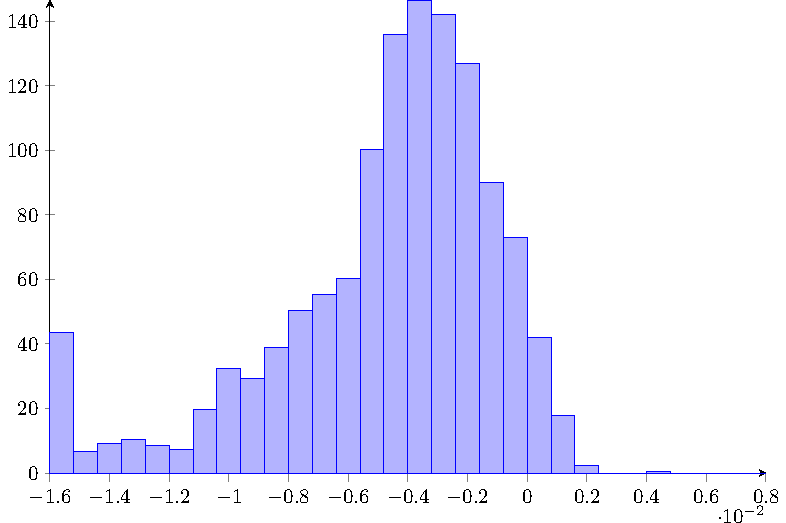
\includegraphics[width=\textwidth]{resnet50histtrain}
\caption{Histogram of change in top-5 training acc.}
\label{fig:resnet50ablation_conv1_top5_train}
\end{subfigure}
~
\begin{subfigure}[b]{0.45\textwidth}
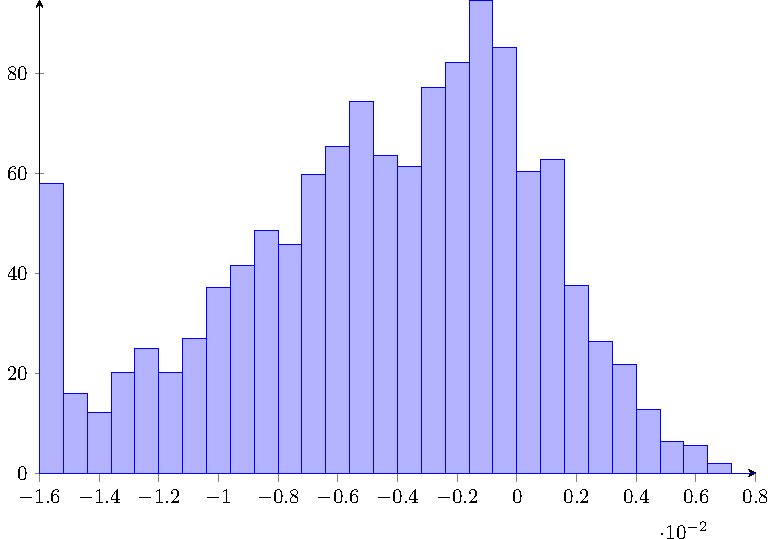
\includegraphics[width=\textwidth]{resnet50histtest}
\caption{Histogram of change in top-5 val.~acc.}
\label{fig:resnet50ablation_conv1_top5_test}
\end{subfigure}

%\input{resnet50fig.tex}
\caption[Pairwise filter ablations in ResNet 50]{Histogram of the change in top-5 accuracy for all pairwise filter ablations of a 2500 randomly sampled images from the ILSVRC training/validation set in \texttt{conv1} of ResNet-50.}
\label{fig:resnet50ablation_conv1_top5}
\end{figure}

While, as expected, most pairwise ablations result in a decrease in accuracy, a small but significant number of pairwise ablations result in an \emph{increase} in accuracy (and decrease in loss). For the validation set this seems to provide clear evidence of hidden units co-adapting, and hence over-fitting to the training data. Surprisingly however, this effect is also evident when evaluating on the training set, and by definition cannot be explained by over-fitting. We observed similar effects on all other layers of the network (see supplemental).


\paragraph{MNIST.} This effect is not limited to large state-of-the-art deep networks, or indeed even deep networks. Surprisingly this effect is reproducible with a minimal single hidden-layer MNIST network. With a fully-connected network with one hidden layer, ReLU activation functions, and a variety of optimization methods, we find that this co-adaption is still present above a minimal number of hidden units.  

\begin{figure}[tp]
\centering
\begin{subfigure}[b]{\linewidth}
\centering
\begin{tikzpicture}

\begin{axis}[
    axis x line=bottom,
    axis y line=left,
    cycle multi list={Set1-5},
    scale only axis,
    width=\linewidth,
    height=0.2\linewidth,
    ylabel={$\max\left(-\Delta L\right)$},
    xmin = 10,
    xmax = 1000,
    ymode=log,
%    xmode=log,
    legend columns=-1,
    legend style={at={(0.5,1.1)},anchor=south,text depth=.5ex},
]
\addplot +[mark=none] table [x index=0, y expr=-\thisrowno{1}, col sep=comma]{ablationdata/mnist/chainer-mnist-ablate-stats_train_loss.log};
\addplot +[mark=none] table [x index=0, y expr=-\thisrowno{1}, col sep=comma]{ablationdata/mnist/chainer-mnist-ablate-momentum-stats_train_loss.log};
\addplot +[mark=none] table [x index=0, y expr=-\thisrowno{1}, col sep=comma]{ablationdata/mnist/chainer-mnist-ablate-wd-stats_train_loss.log};
\addplot +[mark=none] table [x index=0, y expr=-\thisrowno{1}, col sep=comma]{ablationdata/mnist/chainer-mnist-ablate-dropout-stats_train_loss.log};
\addplot +[mark=none] table [x index=0, y expr=-\thisrowno{1}, col sep=comma]{ablationdata/mnist/hessianfree-ablate-mnist-stats_train_loss.log};

\legend{SGD, Momentum, Weight Decay, Dropout, HF}

\end{axis}

\begin{axis}[
    axis x line=none,
    axis y line=right,
    cycle multi list={Set1-5},
    scale only axis,
    width=\linewidth,
    height=0.2\linewidth,
    xlabel={Hidden Units},
    ylabel={$\max\left(\Delta L\right)$},
    xmin = 10,
    xmax = 1000,
    ymode=log,
%    xmode=log,
]

\addplot +[mark=none, dotted] table [x index=0, y expr=\thisrowno{2}, col sep=comma]{ablationdata/mnist/chainer-mnist-ablate-stats_train_loss.log};
\addplot +[mark=none, dotted] table [x index=0, y expr=\thisrowno{2}, col sep=comma]{ablationdata/mnist/chainer-mnist-ablate-momentum-stats_train_loss.log};
\addplot +[mark=none, dotted] table [x index=0, y expr=\thisrowno{2}, col sep=comma]{ablationdata/mnist/chainer-mnist-ablate-wd-stats_train_loss.log};
\addplot +[mark=none, dotted] table [x index=0, y expr=\thisrowno{2}, col sep=comma]{ablationdata/mnist/chainer-mnist-ablate-dropout-stats_train_loss.log};
\addplot +[mark=none, dotted] table [x index=0, y expr=\thisrowno{2}, col sep=comma]{ablationdata/mnist/hessianfree-ablate-mnist-stats_train_loss.log};

\end{axis}


\end{tikzpicture}
\caption{Training Loss Change: Maximum decrease (solid/left axis), and maximum increase (dotted/right axis).}
\label{fig:mnist_ablation_train_loss}
\end{subfigure}


\begin{subfigure}[b]{\linewidth}
\centering
\begin{tikzpicture}
\begin{axis}[
    axis y line=left,
    axis x line=bottom,
    cycle multi list={Set1-5},
    scale only axis,
    width=\linewidth,
    height=0.2\linewidth,
    xlabel={Hidden Units},
    ylabel={$\max\left(\Delta \textrm{Acc.}\right)$},
    xmin = 10,
    xmax = 1000,
    ymode=log,
%    xmode=log,
]

\addplot +[mark=none] table [x index=0, y expr=\thisrowno{2}, col sep=comma]{ablationdata/mnist/chainer-mnist-ablate-stats_train_acc.log};
\addplot +[mark=none] table [x index=0, y expr=\thisrowno{2}, col sep=comma]{ablationdata/mnist/chainer-mnist-ablate-momentum-stats_train_acc.log};
\addplot +[mark=none] table [x index=0, y expr=\thisrowno{2}, col sep=comma]{ablationdata/mnist/chainer-mnist-ablate-wd-stats_train_acc.log};
\addplot +[mark=none] table [x index=0, y expr=\thisrowno{2}, col sep=comma]{ablationdata/mnist/chainer-mnist-ablate-dropout-stats_train_acc.log};
\addplot +[mark=none] table [x index=0, y expr=\thisrowno{2}, col sep=comma]{ablationdata/mnist/hessianfree-ablate-mnist-stats_train_acc.log};

\end{axis}

\begin{axis}[
    axis y line=right,
    axis x line=none,
    cycle multi list={Set1-5},
    scale only axis,
    width=\linewidth,
    height=0.2\linewidth,
    xlabel={Hidden Units},
    ylabel={$\max\left(-\Delta \textrm{Acc.}\right)$},
    xmin = 10,
    xmax = 1000,
    ymode=log,
%    xmode=log,
]
\addplot +[mark=none, dotted] table [x index=0, y expr=-\thisrowno{1}, col sep=comma]{ablationdata/mnist/chainer-mnist-ablate-stats_train_acc.log};
\addplot +[mark=none, dotted] table [x index=0, y expr=-\thisrowno{1}, col sep=comma]{ablationdata/mnist/chainer-mnist-ablate-momentum-stats_train_acc.log};
\addplot +[mark=none, dotted] table [x index=0, y expr=-\thisrowno{1}, col sep=comma]{ablationdata/mnist/chainer-mnist-ablate-wd-stats_train_acc.log};
\addplot +[mark=none, dotted] table [x index=0, y expr=-\thisrowno{1}, col sep=comma]{ablationdata/mnist/chainer-mnist-ablate-dropout-stats_train_acc.log};
\addplot +[mark=none, dotted] table [x index=0, y expr=-\thisrowno{1}, col sep=comma]{ablationdata/mnist/hessianfree-ablate-mnist-stats_train_acc.log};

\end{axis}

\end{tikzpicture}
\caption{Training Accuracy: Maximum increase (solid/left axis), and maximum decrease (dotted/right axis).}
\label{fig:mnist_ablation_train_acc}
\end{subfigure}

% TEST


\begin{subfigure}[b]{\linewidth}
\centering
\begin{tikzpicture}

\begin{axis}[
    axis y line=left,
    axis x line=bottom,
    cycle multi list={Set1-5},
    scale only axis,
    width=\linewidth,
    height=0.2\linewidth,
    xlabel={Hidden Units},
    ylabel={$\max\left(-\Delta L\right)$},
    xmin = 10,
    xmax = 1000,
    ymode=log,
%    xmode=log,
]

\addplot +[mark=none] table [x index=0, y expr=-\thisrowno{1}, col sep=comma]{ablationdata/mnist/chainer-mnist-ablate-stats_test_loss.log};
\addplot +[mark=none] table [x index=0, y expr=-\thisrowno{1}, col sep=comma]{ablationdata/mnist/chainer-mnist-ablate-momentum-stats_test_loss.log};
\addplot +[mark=none] table [x index=0, y expr=-\thisrowno{1}, col sep=comma]{ablationdata/mnist/chainer-mnist-ablate-wd-stats_test_loss.log};
\addplot +[mark=none] table [x index=0, y expr=-\thisrowno{1}, col sep=comma]{ablationdata/mnist/chainer-mnist-ablate-dropout-stats_test_loss.log};
\addplot +[mark=none] table [x index=0, y expr=-\thisrowno{1}, col sep=comma]{ablationdata/mnist/hessianfree-ablate-mnist-stats_test_loss.log};

\end{axis}

\begin{axis}[
    axis y line=right,
    axis x line=none,
    cycle multi list={Set1-5},
    scale only axis,
    width=\linewidth,
    height=0.2\linewidth,
    xlabel={Hidden Units},
    ylabel={$\max\left(\Delta L\right)$},
    xmin = 10,
    xmax = 1000,
    ymode=log,
%    xmode=log,
]

\addplot +[mark=none, dotted] table [x index=0, y expr=\thisrowno{2}, col sep=comma]{ablationdata/mnist/chainer-mnist-ablate-stats_test_loss.log};
\addplot +[mark=none, dotted] table [x index=0, y expr=\thisrowno{2}, col sep=comma]{ablationdata/mnist/chainer-mnist-ablate-momentum-stats_test_loss.log};
\addplot +[mark=none, dotted] table [x index=0, y expr=\thisrowno{2}, col sep=comma]{ablationdata/mnist/chainer-mnist-ablate-wd-stats_test_loss.log};
\addplot +[mark=none, dotted] table [x index=0, y expr=\thisrowno{2}, col sep=comma]{ablationdata/mnist/chainer-mnist-ablate-dropout-stats_test_loss.log};
\addplot +[mark=none, dotted] table [x index=0, y expr=\thisrowno{2}, col sep=comma]{ablationdata/mnist/hessianfree-ablate-mnist-stats_test_loss.log};


\end{axis}

\end{tikzpicture}
\caption{Test Loss: Maximum decrease (solid/left axis), and maximum increase (dotted/right axis).}
\label{fig:mnist_ablation_test_loss}
\end{subfigure}


\begin{subfigure}[b]{\linewidth}
\centering
\begin{tikzpicture}
\begin{axis}[
    axis x line=bottom,
    axis y line=left,
    cycle multi list={Set1-5},
    scale only axis,
    width=\linewidth,
    height=0.2\linewidth,
    xlabel={Hidden Units},
    ylabel={$\max\left(\Delta \textrm{Acc.}\right)$},
    xmin = 10,
    xmax = 1000,
    ymode=log,
%    xmode=log,
]

\addplot +[mark=none] table [x index=0, y expr=\thisrowno{2}, col sep=comma]{ablationdata/mnist/chainer-mnist-ablate-stats_test_acc.log};
\addplot +[mark=none] table [x index=0, y expr=\thisrowno{2}, col sep=comma]{ablationdata/mnist/chainer-mnist-ablate-momentum-stats_test_acc.log};
\addplot +[mark=none] table [x index=0, y expr=\thisrowno{2}, col sep=comma]{ablationdata/mnist/chainer-mnist-ablate-wd-stats_test_acc.log};
\addplot +[mark=none] table [x index=0, y expr=\thisrowno{2}, col sep=comma]{ablationdata/mnist/chainer-mnist-ablate-dropout-stats_test_acc.log};
\addplot +[mark=none] table [x index=0, y expr=\thisrowno{2}, col sep=comma]{ablationdata/mnist/hessianfree-ablate-mnist-stats_test_acc.log};
\end{axis}

\begin{axis}[
    axis y line=right,
    axis x line=none,
    cycle multi list={Set1-5},
    scale only axis,
    width=\linewidth,
    height=0.2\linewidth,
    xlabel={Hidden Units},
    ylabel={$\max\left(-\Delta \textrm{Acc.}\right)$},
    xmin = 10,
    xmax = 1000,
    ymode=log,
%    xmode=log,
]
\addplot +[mark=none, dotted] table [x index=0, y expr=-\thisrowno{1}, col sep=comma]{ablationdata/mnist/chainer-mnist-ablate-stats_test_acc.log};
\addplot +[mark=none, dotted] table [x index=0, y expr=-\thisrowno{1}, col sep=comma]{ablationdata/mnist/chainer-mnist-ablate-momentum-stats_test_acc.log};
\addplot +[mark=none, dotted] table [x index=0, y expr=-\thisrowno{1}, col sep=comma]{ablationdata/mnist/chainer-mnist-ablate-wd-stats_test_acc.log};
\addplot +[mark=none, dotted] table [x index=0, y expr=-\thisrowno{1}, col sep=comma]{ablationdata/mnist/chainer-mnist-ablate-dropout-stats_test_acc.log};
\addplot +[mark=none, dotted] table [x index=0, y expr=-\thisrowno{1}, col sep=comma]{ablationdata/mnist/hessianfree-ablate-mnist-stats_test_acc.log};

\end{axis}

\end{tikzpicture}
\caption{Test Accuracy: Maximum increase (solid/left axis), and maximum decrease (dotted/right axis).}
\label{fig:mnist_ablation_test_acc}
\end{subfigure}


\caption[Pairwise filter ablation for MNIST]{Maximum increase and decrease in training/test loss/accuracy for a single layer hidden MNIST classification network under pairwise ablation of the hidden units. Solid lines show the maximum decrease in loss or increase in accuracy for all pairs of neurons. Dotted lines show the maximum increase in loss or decrease in accuracy. Both are measures of the level of neural co-adpation in the trained networks.}
\label{fig:mnist_ablation}
\end{figure}



\begin{figure}[tp]
\centering

\begin{subfigure}[b]{\linewidth}
\centering
\begin{tikzpicture}

\begin{axis}[
    axis x line=bottom,
    axis y line=left,
    cycle multi list={Set1-5},
    scale only axis,
    width=\linewidth,
    height=0.2\linewidth,
    xlabel={Hidden Units},
    ylabel={\% of pairwise units where $\Delta L < 0$},
    yticklabel=\pgfmathprintnumber{\tick}\,\%,
    xmin = 10,
    xmax = 1000,
%    ymode=log,
%    xmode=log,
    legend columns=-1,
    legend style={at={(0.5,1.1)},anchor=south,text depth=.5ex},
]
\addplot +[mark=none] table [x index=0, y expr=100*\thisrowno{5} / (\thisrowno{0}*\thisrowno{0}), col sep=comma]{ablationdata/mnist/chainer-mnist-ablate-stats_train_loss.log};
\addplot +[mark=none] table [x index=0, y expr=100*\thisrowno{5} / (\thisrowno{0}*\thisrowno{0}), col sep=comma]{ablationdata/mnist/chainer-mnist-ablate-momentum-stats_train_loss.log};
\addplot +[mark=none] table [x index=0, y expr=100*\thisrowno{5} / (\thisrowno{0}*\thisrowno{0}), col sep=comma]{ablationdata/mnist/chainer-mnist-ablate-wd-stats_train_loss.log};
\addplot +[mark=none] table [x index=0, y expr=100*\thisrowno{5} / (\thisrowno{0}*\thisrowno{0}), col sep=comma]{ablationdata/mnist/chainer-mnist-ablate-dropout-stats_train_loss.log};
\addplot +[mark=none] table [x index=0, y expr=100*\thisrowno{5} / (\thisrowno{0}*\thisrowno{0}), col sep=comma]{ablationdata/mnist/hessianfree-ablate-mnist-stats_train_loss.log};

\legend{SGD, Momentum, Weight Decay, Dropout, HF}

\end{axis}

\end{tikzpicture}
\caption{Training Loss: Percentage of pairs of hidden units that exhibit adverse co-adaption.}
\label{fig:mnist_ablation_stats_train_loss_lt}
\end{subfigure}

\begin{subfigure}[b]{\linewidth}
\centering
\begin{tikzpicture}

\begin{axis}[
    axis x line=bottom,
    axis y line=left,
    cycle multi list={Set1-5},
    scale only axis,
    width=\linewidth,
    height=0.2\linewidth,
    xlabel={Hidden Units},
    ylabel={\% of pairwise units where $\Delta L = 0$},
    yticklabel=\pgfmathprintnumber{\tick}\,\%,
    xmin = 10,
    xmax = 1000,
%    ymode=log,
%    xmode=log,
]
\addplot +[mark=none] table [x index=0, y expr=100*\thisrowno{4} / (\thisrowno{0}*\thisrowno{0}), col sep=comma]{ablationdata/mnist/chainer-mnist-ablate-stats_train_loss.log};
\addplot +[mark=none] table [x index=0, y expr=100*\thisrowno{4} / (\thisrowno{0}*\thisrowno{0}), col sep=comma]{ablationdata/mnist/chainer-mnist-ablate-momentum-stats_train_loss.log};
\addplot +[mark=none] table [x index=0, y expr=100*\thisrowno{4} / (\thisrowno{0}*\thisrowno{0}), col sep=comma]{ablationdata/mnist/chainer-mnist-ablate-wd-stats_train_loss.log};
\addplot +[mark=none] table [x index=0, y expr=100*\thisrowno{4} / (\thisrowno{0}*\thisrowno{0}), col sep=comma]{ablationdata/mnist/chainer-mnist-ablate-dropout-stats_train_loss.log};
\addplot +[mark=none] table [x index=0, y expr=100*\thisrowno{4} / (\thisrowno{0}*\thisrowno{0}), col sep=comma]{ablationdata/mnist/hessianfree-ablate-mnist-stats_train_loss.log};

\end{axis}

\end{tikzpicture}
\caption{Training Loss: Percentage of pairs of hidden units that are independent.}
\label{fig:mnist_ablation_stats_train_loss_eq}
\end{subfigure}

\begin{subfigure}[b]{\linewidth}
\centering
\begin{tikzpicture}

\begin{axis}[
    axis x line=bottom,
    axis y line=left,
    cycle multi list={Set1-5},
    scale only axis,
    width=\linewidth,
    height=0.2\linewidth,
    xlabel={Hidden Units},
    ylabel={\% of pairwise units where $\Delta L > 0$},
    yticklabel=\pgfmathprintnumber{\tick}\,\%,
    xmin = 10,
    xmax = 1000,
%    ymode=log,
%    xmode=log,
]
\addplot +[mark=none] table [x index=0, y expr=100*\thisrowno{6} / (\thisrowno{0}*\thisrowno{0}), col sep=comma]{ablationdata/mnist/chainer-mnist-ablate-stats_train_loss.log};
\addplot +[mark=none] table [x index=0, y expr=100*\thisrowno{6} / (\thisrowno{0}*\thisrowno{0}), col sep=comma]{ablationdata/mnist/chainer-mnist-ablate-momentum-stats_train_loss.log};
\addplot +[mark=none] table [x index=0, y expr=100*\thisrowno{6} / (\thisrowno{0}*\thisrowno{0}), col sep=comma]{ablationdata/mnist/chainer-mnist-ablate-wd-stats_train_loss.log};
\addplot +[mark=none] table [x index=0, y expr=100*\thisrowno{6} / (\thisrowno{0}*\thisrowno{0}), col sep=comma]{ablationdata/mnist/chainer-mnist-ablate-dropout-stats_train_loss.log};
\addplot +[mark=none] table [x index=0, y expr=100*\thisrowno{6} / (\thisrowno{0}*\thisrowno{0}), col sep=comma]{ablationdata/mnist/hessianfree-ablate-mnist-stats_train_loss.log};

\end{axis}

\end{tikzpicture}
\caption{Training Loss: Percentage of pairs of hidden units that are codependent.}
\label{fig:mnist_ablation_stats_train_loss_gt}
\end{subfigure}

\caption[Pairwise filter ablation counts for MNIST]{Number of pairs of hidden units in a single layer hidden MNIST classification network which under ablation, are adversely dependent ($\Delta L < 0$), independent ($\Delta L = 0$) or dependent ($\Delta L > 0$) for the training set.}
\label{fig:mnist_ablation_stats}
\end{figure}

\cref{fig:mnist_ablation} shows the minimum and maximum increase in training loss/accuracy and test loss/accuracy for the MNIST network with different numbers of hidden units, when pairwise filters are ablated, as evaluated on the entire MNIST training/test sets. The effect of training with weight decay, dropout and momentum are also compared with vanilla SGD. Weight decay and dropout are considered to be regularization methods, while momentum is an optimization trick that is intended to help avoid some issues of using a first order optimization -- it can help speed up learning in the presence of some types of pathological curvature that would otherwise lead to slow optimization or a poor local minima with vanilla SGD.

Momentum clearly helps avoid co-adaption the most, with there being no increase in accuracy/decrease in loss at training time, as compared to vanilla SGD where co-adaption is significant. Taken by itself, this observation would indicate that co-adaption is a symptom of an optimization problem. Weight decay does not seem to have a helpful effect on co-adaption, if anything it may exacerbate the phenomenon. As a form of regularization, this might be expected, as it should help generalization, not training fit. On the other hand Dropout seems to reduce the number of co-adapted units significantly, and is even effective at reducing co-adaption at \emph{training time}. If dropout is a regularization method, then this seems to conflict with our findings from weight decay and momentum.

\subsection{Dropout as an optimization trick}
Dropout can also be thought of as a orthogonal projection of the error surface onto a random lower-dimensional subspace, in which the curvature of the error surface may no longer exhibit pathological issues, and optimization may be easier. For example, if in a subset of the dimensions, a deep valley exists, and these dimensions are dropped-out. Random projection is a well established method for dimensionality reduction of high dimensional spaces~\citep{kaski1998dimensionality,fodor2002survey}.
If a layer has $N$ nodes, and a weight matrix $W$, and input vector $x$, then dropout on the layer of $K/N$ nodes may be defined as the transformation:

\begin{equation}
    \textrm{Dropout}(\mathbf{W}) = \mathbf{D}_{i} \mathbf{W},
\end{equation}

where $D$ is a diagonal binary matrix, with rank $K$, defining an orthogonal projection onto a $K$-dimensional subspace. 

To demonstrate that it is this projection, rather than the zeroing out of neurons itself, that is responsible for performance improvements with dropout, we can instead perform a random projection in a different orthogonal co-ordinate basis, which does not dropout (zero) any neurons. To do this we can first rotate the parameters with random rotation matrix into a non-axis aligned co-ordinate basis, and perform dropout (orthogonal projection) in the rotated space, and then rotate back into the original co-ordinate basis:

\begin{equation}
    \textrm{Dropproject}(\mathbf{W}_l) = \mathbf{R}^{-1}\textrm{Dropout}(\mathbf{R} \mathbf{W}_l),
\end{equation}

for a random rotation matrix $\mathbf{R}\in \textrm{SO}_N$. ``Dropproject'' avoids zeroing out any of the units, while still performing an equivalent projection as that in dropout.

\begin{figure}[tp]

\begin{subfigure}[b]{\linewidth}
\begin{tikzpicture}
\begin{axis}[
    thick,
    cycle multi list={Set1-5},
    scale only axis,
    axis x line=bottom,
    axis y line=left,
    %axis line style={thick},
    width=\linewidth,
    height=0.2\linewidth,
    xlabel={Epochs},
    ylabel={Log Loss},
    ymode=log,
    legend columns=-1,
    legend style={at={(0.5,1.1)},anchor=south,text depth=.5ex},
]

\addplot +[mark=none] table [x=epoch, y expr=\thisrow{main/loss}, col sep=comma]{ablationdata/dropproject/train_standard.csv};
\addplot +[mark=none] table [x=epoch, y expr=\thisrow{main/loss}, col sep=comma]{ablationdata/dropproject/train_dropout.csv};
\addplot +[mark=none] table [x=epoch, y expr=\thisrow{main/loss}, col sep=comma]{ablationdata/dropproject/train_dropproject.csv};
\addplot +[mark=none] table [x=epoch, y expr=\thisrow{main/loss}, col sep=comma]{ablationdata/dropproject/train_dropproject10.csv};
\addplot +[mark=none] table [x=epoch, y expr=\thisrow{main/loss}, col sep=comma]{ablationdata/dropproject/train_dropprojectrandom.csv};

\legend{
Standard, 
Dropout, 
Dropproject,
DP-Random 10,
DP-Random}

\end{axis}

\end{tikzpicture}
\caption{CIFAR Training Log Loss}
\label{fig:cifar_dropproject_train_loss}
\end{subfigure}

\begin{subfigure}[b]{\linewidth}

\begin{tikzpicture}
\begin{axis}[
    thick,
    cycle multi list={Set1-9},
    scale only axis,
    axis x line=bottom,
    axis y line=left,
    %axis line style={thick},
    width=\linewidth,
    height=0.2\linewidth,
    xlabel={Epochs},
    ylabel={Log Loss},
    ymode=log,
%    ymax=1,
    ymin=0,
]

\addplot +[mark=none] table [x=epoch, y expr=\thisrow{validation/main/loss}, col sep=comma]{ablationdata/dropproject/train_standard.csv};
\addplot +[mark=none] table [x=epoch, y expr=\thisrow{validation/main/loss}, col sep=comma]{ablationdata/dropproject/train_dropout.csv};
\addplot +[mark=none] table [x=epoch, y expr=\thisrow{validation/main/loss}, col sep=comma]{ablationdata/dropproject/train_dropproject.csv};
\addplot +[mark=none] table [x=epoch, y expr=\thisrow{validation/main/loss}, col sep=comma]{ablationdata/dropproject/train_dropproject10.csv};
\addplot +[mark=none] table [x=epoch, y expr=\thisrow{validation/main/loss}, col sep=comma]{ablationdata/dropproject/train_dropprojectrandom.csv};

\end{axis}
\end{tikzpicture}

\caption{CIFAR Test Log Loss}
\label{fig:cifar_dropproject_test_loss}
\end{subfigure}

\begin{subfigure}[b]{\linewidth}
\begin{tikzpicture}
\begin{axis}[
    thick,
    cycle multi list={Set1-9},
    scale only axis,
    axis x line=bottom,
    axis y line=left,
    %axis line style={thick},
    width=\linewidth,
    height=0.2\linewidth,
    xlabel={Epochs},
    ylabel={Training Error},
%    ymax=1,
%    ymin=0,
]

\addplot +[mark=none] table [x=epoch, y expr=1-\thisrow{main/accuracy}, col sep=comma]{ablationdata/dropproject/train_standard.csv};
\addplot +[mark=none] table [x=epoch, y expr=1-\thisrow{main/accuracy}, col sep=comma]{ablationdata/dropproject/train_dropout.csv};
\addplot +[mark=none] table [x=epoch, y expr=1-\thisrow{main/accuracy}, col sep=comma]{ablationdata/dropproject/train_dropproject.csv};
\addplot +[mark=none] table [x=epoch, y expr=1-\thisrow{main/accuracy}, col sep=comma]{ablationdata/dropproject/train_dropproject10.csv};
\addplot +[mark=none] table [x=epoch, y expr=1-\thisrow{main/accuracy}, col sep=comma]{ablationdata/dropproject/train_dropprojectrandom.csv};

\end{axis}

\end{tikzpicture}
\caption{CIFAR Training Error}
\label{fig:cifar_dropproject_train_acc}
\end{subfigure}

\begin{subfigure}[b]{\linewidth}

\begin{tikzpicture}
\begin{axis}[
    thick,
    cycle multi list={Set1-9},
    scale only axis,
    axis x line=bottom,
    axis y line=left,
    %axis line style={thick},
    width=\linewidth,
    height=0.2\linewidth,
    xlabel={Epochs},
    ylabel={Test Error},
%    ymin = 0,
]

\addplot +[mark=none] table [x=epoch, y expr=1-\thisrow{validation/main/accuracy}, col sep=comma]{ablationdata/dropproject/train_standard.csv};
\addplot +[mark=none] table [x=epoch, y expr=1-\thisrow{validation/main/accuracy}, col sep=comma]{ablationdata/dropproject/train_dropout.csv};
\addplot +[mark=none] table [x=epoch, y expr=1-\thisrow{validation/main/accuracy}, col sep=comma]{ablationdata/dropproject/train_dropproject.csv};
\addplot +[mark=none] table [x=epoch, y expr=1-\thisrow{validation/main/accuracy}, col sep=comma]{ablationdata/dropproject/train_dropproject10.csv};
\addplot +[mark=none] table [x=epoch, y expr=1-\thisrow{validation/main/accuracy}, col sep=comma]{ablationdata/dropproject/train_dropprojectrandom.csv};

\end{axis}
\end{tikzpicture}

\caption{CIFAR Test Error}
\label{fig:cifar_dropproject_test_acc}
\end{subfigure}

\caption[Dropout \vs dropproject for VGG/CIFAR-10]{Training and test curves for a VGG network on CIFAR comparing dropout to dropproject.}
\label{fig:cifar_dropproject}
\end{figure}

\cref{fig:cifar_dropproject} compares the effect of dropout, and various forms of dropproject, on a large VGG model trained on the CIFAR-10~\citep{CIFAR10} dataset. Both dropout and dropproject are only applied to the two large fully connected layers of the VGG network. With \textbf{Dropproject}, one random rotation matrix is generated and used for the duration of training. For \textbf{DP-Random10}, 10 random rotation matrices are generated and a single rotation matrix is randomly chosen from these for each mini-batch during training. Finally, \textbf{DP-Random} generates a random rotation matrix for each mini-batch.

Both methods have close to identical effect on training loss/error, and are drastically different than the plots of the standard network without dropout/dropproject. At test time, both methods also achieve comparable minimum error, but in the loss curve it can be seen that dropproject appears to start overfitting earlier than dropout. While the projection (and not regularization) appears to be responsible for the increased generalization and speed of training, the zeroing out of units for dropout also has a small regularization effect not seen in dropproject. None of the variants of dropproject seem to be different, indicating that the random projection itself rather than the random rotation into a different co-ordinate basis is important for the effect.

\paragraph{Dropout and Batch Normalization.}
It has been observed empirically by \citet{Ioffe2015} and others that when used with batch normalization, dropout is not as effective. In light of our understanding of dropout as being an optimization method for error surfaces with highly complex curvature, we can explain this. As explained by~\citep{martens2010deep}, an important property of second order optimization methods is ``scale invariance'' -- robustness to any linear rescaling of the model parameters. For example, if we are in an elliptically shaped local minima of the error surface, ideally we would want different a higher learning rate for parameters in the direction of the major axis, as compared to those in the direction of the minor axis, as RMSprop attempts. When using batch normalization, the layer-wise error surface is whitened, reducing the importance of scale-invariance in optimization.

\mynote{Questions to answer:
\begin{itemize}
\item Do residual connections alleviate neural co-adaption?
\item Learning identity mapping is difficult due to bad curvature, exact situation cited as example by \citet{martens2010deep}.
\item Is learning deep networks easier than learning wide networks because of neural co-adaption?
\end{itemize}}

\end{document}

%\include{Chapter7/chapter7}



% ********************************** Back Matter *******************************
% Backmatter should be commented out, if you are using appendices after References
%\backmatter

% ********************************** Bibliography ******************************
\begin{spacing}{0.9}

% To use the conventional natbib style referencing
% Bibliography style previews: http://nodonn.tipido.net/bibstyle.php
% Reference styles: http://sites.stat.psu.edu/~surajit/present/bib.htm

\bibliographystyle{apalike}
%\bibliographystyle{plainnat} % use this to have URLs listed in References
\cleardoublepage
\bibliography{References/references} % Path to your References.bib file


% If you would like to use BibLaTeX for your references, pass `custombib' as
% an option in the document class. The location of 'reference.bib' should be
% specified in the preamble.tex file in the custombib section.
% Comment out the lines related to natbib above and uncomment the following line.

%\printbibliography[heading=bibintoc, title={References}]


\end{spacing}

% ********************************** Appendices ********************************

\begin{appendices} % Using appendices environment for more functunality

%% ******************************* Thesis Appendix A ****************************
\chapter{How to install \LaTeX} 

\section*{Windows OS}

\subsection*{TeXLive package - full version}
\begin{enumerate}
\item	Download the TeXLive ISO (2.2GB) from\\
\href{https://www.tug.org/texlive/}{https://www.tug.org/texlive/}
\item	Download WinCDEmu (if you don't have a virtual drive) from \\
\href{http://wincdemu.sysprogs.org/download/}
{http://wincdemu.sysprogs.org/download/}
\item	To install Windows CD Emulator follow the instructions at\\
\href{http://wincdemu.sysprogs.org/tutorials/install/}
{http://wincdemu.sysprogs.org/tutorials/install/}
\item	Right click the iso and mount it using the WinCDEmu as shown in \\
\href{http://wincdemu.sysprogs.org/tutorials/mount/}{
http://wincdemu.sysprogs.org/tutorials/mount/}
\item	Open your virtual drive and run setup.pl
\end{enumerate}

or

\subsection*{Basic MikTeX - \TeX~ distribution}
\begin{enumerate}
\item	Download Basic-MiK\TeX (32bit or 64bit) from\\
\href{http://miktex.org/download}{http://miktex.org/download}
\item	Run the installer 
\item	To add a new package go to Start >> All Programs >> MikTex >> Maintenance (Admin) and choose Package Manager
\item	Select or search for packages to install
\end{enumerate}

\subsection*{TexStudio - \TeX~ editor}
\begin{enumerate}
\item	Download TexStudio from\\
\href{http://texstudio.sourceforge.net/\#downloads}
{http://texstudio.sourceforge.net/\#downloads} 
\item	Run the installer
\end{enumerate}

\section*{Mac OS X}
\subsection*{MacTeX - \TeX~ distribution}
\begin{enumerate}
\item	Download the file from\\
\href{https://www.tug.org/mactex/}{https://www.tug.org/mactex/}
\item	Extract and double click to run the installer. It does the entire configuration, sit back and relax.
\end{enumerate}

\subsection*{TexStudio - \TeX~ editor}
\begin{enumerate}
\item	Download TexStudio from\\
\href{http://texstudio.sourceforge.net/\#downloads}
{http://texstudio.sourceforge.net/\#downloads} 
\item	Extract and Start
\end{enumerate}


\section*{Unix/Linux}
\subsection*{TeXLive - \TeX~ distribution}
\subsubsection*{Getting the distribution:}
\begin{enumerate}
\item	TexLive can be downloaded from\\
\href{http://www.tug.org/texlive/acquire-netinstall.html}
{http://www.tug.org/texlive/acquire-netinstall.html}.
\item	TexLive is provided by most operating system you can use (rpm,apt-get or yum) to get TexLive distributions
\end{enumerate}

\subsubsection*{Installation}
\begin{enumerate}
\item	Mount the ISO file in the mnt directory
\begin{verbatim}
mount -t iso9660 -o ro,loop,noauto /your/texlive####.iso /mnt
\end{verbatim}

\item	Install wget on your OS (use rpm, apt-get or yum install)
\item	Run the installer script install-tl.
\begin{verbatim}
	cd /your/download/directory
	./install-tl
\end{verbatim}
\item	Enter command `i' for installation

\item	Post-Installation configuration:\\
\href{http://www.tug.org/texlive/doc/texlive-en/texlive-en.html\#x1-320003.4.1}
{http://www.tug.org/texlive/doc/texlive-en/texlive-en.html\#x1-320003.4.1} 
\item	Set the path for the directory of TexLive binaries in your .bashrc file
\end{enumerate}

\subsubsection*{For 32bit OS}
For Bourne-compatible shells such as bash, and using Intel x86 GNU/Linux and a default directory setup as an example, the file to edit might be \begin{verbatim}
edit $~/.bashrc file and add following lines
PATH=/usr/local/texlive/2011/bin/i386-linux:$PATH; 
export PATH 
MANPATH=/usr/local/texlive/2011/texmf/doc/man:$MANPATH;
export MANPATH 
INFOPATH=/usr/local/texlive/2011/texmf/doc/info:$INFOPATH;
export INFOPATH
\end{verbatim}
\subsubsection*{For 64bit OS}
\begin{verbatim}
edit $~/.bashrc file and add following lines
PATH=/usr/local/texlive/2011/bin/x86_64-linux:$PATH;
export PATH 
MANPATH=/usr/local/texlive/2011/texmf/doc/man:$MANPATH;
export MANPATH 
INFOPATH=/usr/local/texlive/2011/texmf/doc/info:$INFOPATH;
export INFOPATH

\end{verbatim}



%\subsection{Installing directly using Linux packages} 
\subsubsection*{Fedora/RedHat/CentOS:}
\begin{verbatim} 
sudo yum install texlive 
sudo yum install psutils 
\end{verbatim}


\subsubsection*{SUSE:}
\begin{verbatim}
sudo zypper install texlive
\end{verbatim}


\subsubsection*{Debian/Ubuntu:}
\begin{verbatim} 
sudo apt-get install texlive texlive-latex-extra 
sudo apt-get install psutils
\end{verbatim}

%% ******************************* Thesis Appendix B ********************************

\chapter{Installing the CUED class file}

\LaTeX.cls files can be accessed system-wide when they are placed in the
<texmf>/tex/latex directory, where <texmf> is the root directory of the user’s \TeX installation. On systems that have a local texmf tree (<texmflocal>), which
may be named ``texmf-local'' or ``localtexmf'', it may be advisable to install packages in <texmflocal>, rather than <texmf> as the contents of the former, unlike that of the latter, are preserved after the \LaTeX system is reinstalled and/or upgraded.

It is recommended that the user create a subdirectory <texmf>/tex/latex/CUED for all CUED related \LaTeX class and package files. On some \LaTeX systems, the directory look-up tables will need to be refreshed after making additions or deletions to the system files. For \TeX Live systems this is accomplished via executing ``texhash'' as root. MIK\TeX users can run ``initexmf -u'' to accomplish the same thing.

Users not willing or able to install the files system-wide can install them in their personal directories, but will then have to provide the path (full or relative) in addition to the filename when referring to them in \LaTeX.



\end{appendices}

% *************************************** Index ********************************
\printthesisindex % If index is present

\end{document}
